\documentclass[a4paper]{article}
\usepackage[ngerman]{babel}
\usepackage[utf8]{inputenc}
\usepackage{multicol}
\usepackage{calc}
\usepackage{ifthen}
\usepackage[landscape]{geometry}
\usepackage{amsmath,amsthm,amsfonts,amssymb}
\usepackage{color,graphicx,overpic}
\usepackage{xcolor, listings}
\usepackage[compact]{titlesec} %less space for headers
\usepackage{mdwlist} %less space for lists
\usepackage{pdflscape}
\usepackage{verbatim}
\usepackage[most]{tcolorbox}
\usepackage[hidelinks,pdfencoding=auto]{hyperref}
\usepackage{bussproofs}
\usepackage{fancyhdr}
\usepackage{lastpage}
\pagestyle{fancy}
\fancyhf{}
\fancyhead[L]{Advanced Operating Systems}
\fancyfoot[L]{\thepage/\pageref{LastPage}}
\renewcommand{\headrulewidth}{0pt} %obere Trennlinie
\renewcommand{\footrulewidth}{0pt} %untere Trennlinie

\usepackage{pifont}
\newcommand{\cmark}{\ding{51}}
\newcommand{\xmark}{\ding{55}}

\pdfinfo{
 /Title (Advanced Operating Systems - Cheatsheet)
 /Creator (TeX)
 /Producer (pdfTeX 1.40.0)
 /Author (Robert Jeutter)
 /Subject ()
}

%%% Code Listings
\definecolor{codegreen}{rgb}{0,0.6,0}
\definecolor{codegray}{rgb}{0.5,0.5,0.5}
\definecolor{codepurple}{rgb}{0.58,0,0.82}
\definecolor{backcolour}{rgb}{0.95,0.95,0.92}
\lstdefinestyle{mystyle}{
 backgroundcolor=\color{backcolour}, 
 commentstyle=\color{codegreen},
 keywordstyle=\color{magenta},
 numberstyle=\tiny\color{codegray},
 stringstyle=\color{codepurple},
 basicstyle=\ttfamily,
 breakatwhitespace=false, 
}
\lstset{style=mystyle, upquote=true}

%textmarker style from colorbox doc
\tcbset{textmarker/.style={%
 enhanced,
 parbox=false,boxrule=0mm,boxsep=0mm,arc=0mm,
 outer arc=0mm,left=2mm,right=2mm,top=3pt,bottom=3pt,
 toptitle=1mm,bottomtitle=1mm,oversize}}

% define new colorboxes
\newtcolorbox{hintBox}{textmarker,
 borderline west={6pt}{0pt}{yellow},
 colback=yellow!10!white}
\newtcolorbox{importantBox}{textmarker,
 borderline west={6pt}{0pt}{red},
 colback=red!10!white}
\newtcolorbox{noteBox}{textmarker,
 borderline west={3pt}{0pt}{green},
 colback=green!10!white}

% define commands for easy access
\renewcommand{\note}[2]{\begin{noteBox} \textbf{#1} #2 \end{noteBox}}
\newcommand{\warning}[1]{\begin{hintBox} \textbf{Warning:} #1 \end{hintBox}}
\newcommand{\important}[1]{\begin{importantBox} \textbf{Important:} #1 \end{importantBox}}

% This sets page margins to .5 inch if using letter paper, and to 1cm
% if using A4 paper. (This probably isn't strictly necessary.)
% If using another size paper, use default 1cm margins.
\ifthenelse{\lengthtest { \paperwidth = 11in}}
 { \geometry{top=.5in,left=.5in,right=.5in,bottom=.5in} }
 {\ifthenelse{ \lengthtest{ \paperwidth = 297mm}}
 {\geometry{top=1.3cm,left=1cm,right=1cm,bottom=1.2cm} }
 {\geometry{top=1.3cm,left=1cm,right=1cm,bottom=1.2cm} }
 }

% Redefine section commands to use less space
\makeatletter
\renewcommand{\section}{\@startsection{section}{1}{0mm}%
 {-1ex plus -.5ex minus -.2ex}%
 {0.5ex plus .2ex}%x
 {\normalfont\large\bfseries}}
\renewcommand{\subsection}{\@startsection{subsection}{2}{0mm}%
 {-1explus -.5ex minus -.2ex}%
 {0.5ex plus .2ex}%
 {\normalfont\normalsize\bfseries}}
\renewcommand{\subsubsection}{\@startsection{subsubsection}{3}{0mm}%
 {-1ex plus -.5ex minus -.2ex}%
 {1ex plus .2ex}%
 {\normalfont\small\bfseries}}
\makeatother

% Don't print section numbers
\setcounter{secnumdepth}{0}

\setlength{\parindent}{0pt}
\setlength{\parskip}{0pt plus 0.5ex} 
% compress space
\setlength\abovedisplayskip{0pt}
\setlength{\parskip}{0pt}
\setlength{\parsep}{0pt}
\setlength{\topskip}{0pt}
\setlength{\topsep}{0pt}
\setlength{\partopsep}{0pt}
\linespread{0.5}
\titlespacing{\section}{0pt}{*0}{*0}
\titlespacing{\subsection}{0pt}{*0}{*0}
\titlespacing{\subsubsection}{0pt}{*0}{*0}

\begin{document}

\raggedright
\begin{multicols}{3}\scriptsize % multicol parameters % These lengths are set only within the two main columns %\setlength{\columnseprule}{0.25pt} \setlength{\premulticols}{1pt} \setlength{\postmulticols}{1pt} \setlength{\multicolsep}{1pt} \setlength{\columnsep}{2pt} 

    \subsection{Funktionale und nichtfunktionale Eigenschaften}
    \begin{itemize*}
        \item Requirements: (nicht-)Funktionale Eigenschaften entstehen durch Erfüllung von (nicht-)funktionalen Anforderungen
        \item funktionale Eigenschaft: was ein Produkt tun soll
        \item nichtfunktionale Eigenschaft (NFE): wie ein Produkt dies tun soll
        \item andere Bezeichnungen NFE: Qualitäten, Quality of Service
    \end{itemize*}

    \subsubsection{Hardwarebasis}
    \begin{itemize*}
        \item Einst: Einprozessor-Systeme
        \item Heute: Mehrprozessor-/hochparallele Systeme
        \item neue Synchronisationsmechanismen erforderlich
        \item $\rightarrow$ unterschiedliche Hardware und deren Multiplexing
    \end{itemize*}

    \subsubsection{Betriebssystemarchitektur}
    \begin{itemize*}
        \item Einst: Monolithische und Makrokernel-Architekturen
        \item Heute: Mikrokernel(-basierte) Architekturen
        \item Exokernelbasierte Architekturen (Library-Betriebssysteme)
        \item Virtualisierungsarchitekturen
        \item Multikernel-Architekturen
        \item $\rightarrow$ unterschiedliche Architekturen
    \end{itemize*}

    \subsubsection{Ressourcenverwaltung}
    \begin{itemize*}
        \item Einst: Batch-Betriebssysteme, Stapelverarbeitung (FIFO)
        \item Heute: Echtzeitgarantien für Multimedia und Sicherheit
        \item echtzeitfähige Scheduler, Hauptspeicherverwaltung, Ereignismanagement, Umgang mit Überlast/Prioritätsumkehr ...
        \item $\rightarrow$ unterschiedliche Ressourcenverwaltung
    \end{itemize*}

    \subsubsection{Betriebssystemabstraktionen}
    \begin{itemize*}
        \item Reservierung von Ressourcen ( $\rightarrow$ eingebettete Systeme)
        \item Realisierung von QoS-Anforderungen ( $\rightarrow$ Multimediasysteme)
        \item Erhöhung der Ausfallsicherheit ( $\rightarrow$ verfügbarkeitskritisch)
        \item Schutz vor Angriffen und Missbrauch ( $\rightarrow$ sicherheitskritisch)
        \item flexiblen und modularen Anpassen des BS ( $\rightarrow$ hochadaptiv)
        \item $\rightarrow$ höchst diverse Abstraktionen von Hardware
    \end{itemize*}

    \subsubsection{Betriebssysteme als Softwareprodukte}
    \begin{itemize*}
        \item Betriebssystem: endliche Menge von Quellcode
        \item besitzen differenzierte Aufgaben $\rightarrow$ funktionale Eigenschaften
        \item Anforderungen an Nutzung und Pflege $\rightarrow$ Evolutionseigenschaften
        \item können für Betriebssysteme höchst speziell sein
        \item $\rightarrow$ spezielle Anforderungen an das Softwareprodukt BS
    \end{itemize*}

    Grundlegende funktionale Eigenschaften von BS: Hardware-
    \begin{description*}
        \item[Abstraktion] Ablaufumgebung auf Basis der Hardware bereitstellen
        \item[Multiplexing] Ablaufumgebung zeitlich/logisch getrennt einzelnen Anwendungen zuteilen
        \item[Schutz] gemeinsame Ablaufumgebung gegen Fehler und Manipulation
    \end{description*}

    Nichtfunktionale Eigenschaften (Auswahl) von Betriebssystemen:
    \begin{itemize*}
        \item Laufzeiteigenschaften: zur Laufzeit eines Systems beobachtbar
        \begin{itemize*}
            \item Sparsamkeit und Effizienz
            \item Robustheit, Verfügbarkeit
            \item Sicherheit (Security)
            \item Echtzeitfähigkeit, Adaptivität, Performanz
        \end{itemize*}
        \item Evolutionseigenschaften: charakterisieren (Weiter-) Entwicklung- und Betrieb eines Systems
        \begin{itemize*}
            \item Wartbarkeit, Portierbarkeit
            \item Offenheit, Erweiterbarkeit
        \end{itemize*}
    \end{itemize*}

    \section{Sparsamkeit und Effizienz}
    \subsection{Motivation}
    Sparsamkeit (Arbeitsdefinition): Die Eigenschaft eines Systems, seine
    Funktion mit minimalem Ressourcenverbrauch auszuüben $\rightarrow$ Effizienz bei Nutzung der Ressourcen

    Effizienz: Der Grad, zu welchem ein System oder eine seiner Komponenten
    seine Funktion mit minimalem Ressourcenverbrauch ausübt. (IEEE)

    Beispiele:
    \begin{itemize*}
        \item mobile Geräte: Sparsamkeit mit Energie
        \item Sparsamkeit mit weiteren Ressourcen, z.B. Speicherplatz
        \item Betriebssystem (Kernel + User Space): geringer Speicherbedarf
        \item optimale Speicherverwaltung durch Betriebssystem zur Laufzeit
        \item Baugrößenoptimierung(Platinen-und Peripheriegerätegröße)
        \item Kostenoptimierung(kleine Caches, keine MMU, ...)
        \item massiv reduzierte HW-Schnittstellen (E/A-Geräte, Peripherie)
    \end{itemize*}

    Mobile und eingebettete Systeme (kleine Auswahl)
    \begin{itemize*}
        \item mobile Rechner-Endgeräte
        \item Weltraumfahrt und -erkundung
        \item Automobile
        \item verteilte Sensornetze (WSN)
        \item Chipkarten
        \item Multimedia-und Unterhaltungselektronik
    \end{itemize*}

    \subsection{Energieeffizienz}
    zeitweiliges Abschalten momentan nicht benötigter Ressourcen

    Betriebssystemmechanismen
    \begin{enumerate*}
        \item Dateisystem-E/A: energieeffizientes Festplatten-Prefetching
        \item CPU-Scheduling: energieeffizientes Scheduling
        \item Speicherverwaltung: Lokalitätsoptimierung
        \item Netzwerk: energiebewusstes Routing
        \item Verteiltes Rechnen: temperaturabhängige Lastverteilung
    \end{enumerate*}

    \subsubsection{Energieeffiziente Dateizugriffe}
    HDD/Netzwerkgeräte/... sparen nur bei relativ langer Inaktivität Energie
    \begin{itemize*}
        \item Aufgabe: kurze, intensive Zugriffsmuster $\rightarrow$ lange Inaktivität
        \item HDD-Geräten: Zustände mit absteigendem Energieverbrauch:
        \begin{enumerate*}
            \item Aktiv: einziger Arbeitszustand
            \item Idle: Platte rotiert, Elektronik teilweise abgeschaltet
            \item Standby: Rotation abgeschaltet
            \item Sleep: gesamte restliche Elektronik abgeschaltet
        \end{enumerate*}
        \item ähnliche, noch stärker differenzierte Zustände bei DRAM
        %\item \includegraphics[width=\linewidth]{Assets/AdvancedOperatingSystems-energiezustände-festplatte.png}
        \item durch geringe Verlängerungen des idle - Intervalls kann signifikant der Energieverbrauch reduziert werden
    \end{itemize*}

    \subsubsection{Prefetching-Mechanismus}
    \begin{itemize*}
        \item Prefetching (,,Speichervorgriff'', vorausschauend) \& Caching
        \begin{itemize*}
            \item Standard-Praxis bei moderner Datei-E/A
            \item Voraussetzung: Vorwissen über benötigte Folge von zukünftigen Datenblockreferenzen
            \item Ziel: Performanzverbesserung durch Durchsatzerhöhung und Latenzzeit-Verringerung
            \item Idee: Vorziehen möglichst vieler E/A-Anforderungen an Festplatte + zeitlich gleichmäßige Verteilung verbleibender
            \item Umsetzung: Caching dieser vorausschauend gelesenen Blöcke in ungenutzten PageCache
        \end{itemize*}
        \item Folge: Inaktivität überwiegend sehr kurz $\rightarrow$ Energieeffizienz ...?
        \item Zugriffs-/Festplattenoperationen
        \begin{itemize*}
            \item access(x) ... greife auf Inhalt von Festplattenblock x im PageCache zu
            \item fetch(x) ... hole Block x nach einem access(x) von Festplatte
            \item prefetch(x) ... hole Block x ohne access(x) von Festplatte
        \end{itemize*}
        \item Fetch-on-Demand-Strategie bisher (kein vorausschauendes Lesen)
        \item Traditionelles Prefetching
        \begin{itemize*}
            \item traditionelle Prefetching-Strategie: bestimmt
            \begin{itemize*}
                \item wann Block von der Platte holen (HW aktiv)
                \item welcher Block zu holen ist
                \item welcher Block zu ersetzen ist
            \end{itemize*}
        \end{itemize*}
            \begin{enumerate*}
                \item Optimales Prefetching: Jedes \emph{prefetch} sollte den nächsten Block im Referenzstrom in den Cache bringen, der noch nicht dort ist
                \item Optimales Ersetzen: Bei jedem ersetzenden \emph{prefetch} sollte der Block überschrieben werden, der am spätesten in der Zukunft wieder benötigt wird
                \item ,,Richte keinen Schaden an'': Überschreibe niemals Block A um Block B zu holen, wenn A vor B benötigt wird
                \item Erste Möglichkeit: Führe nie ein ersetzendes \emph{prefetch} aus, wenn dieses schon vorher hätte ausgeführt werden können
            \end{enumerate*}
        \item Energieeffizientes Prefetching
        \begin{itemize*}
            \item versucht Länge der Disk-Idle-Intervalle zu maximieren
        \end{itemize*}
            \begin{enumerate*}
                \item Optimales Prefetching: Jedes \emph{prefetch} sollte den nächsten Block im Referenzstrom in den Cache bringen, der noch nicht dort ist
                \item Optimales Ersetzen: Bei jedem ersetzenden \emph{prefetch} sollte der Block überschrieben werden, der am spätesten in der Zukunft wieder benötigt wird
                \item ,,Richte keinen Schaden an'': Überschreibe niemals Block A um Block B zu holen, wenn A vor B benötigt wird
                \item Maximiere Zugriffsfolgen: Führe immer dann nach einem \emph{fetch}/\emph{prefetch} ein weiteres \emph{prefetch} aus, wenn Blöcke für eine Ersetzung geeignet sind
                \item Beachte Idle-Zeiten: Unterbrich nur dann eine Inaktivitätsperiode durch ein \emph{prefetch}, falls dieses sofort ausgeführt werden muss, um Cache-Miss zu vermeiden
            \end{enumerate*}
    \end{itemize*}
    Allgemeine Schlussfolgerungen
    \begin{enumerate*}
        \item Hardware-Spezifikation nutzen: Modi, in denen wenig Energie verbraucht wird
        \item Entwicklung von Strategien, die langen Aufenthalt in energiesparenden Modi ermöglichen und dabei Leistungsparameter in vertretbarem Umfang reduzieren
        \item Implementieren dieser Strategien in Betriebssystemmechanismen zur Ressourcenverwaltung
    \end{enumerate*}

    \subsubsection{Energieeffizientes Prozessormanagement}
    Hardware-Gegebenheiten
    \begin{itemize*}
        \item z.Zt. meistgenutzte Halbleitertechnologie für Prozessor-Hardware: CMOS
        ( Complementary Metal Oxide Semiconductor)
        \item
        Komponenten für Energieverbrauch: \$P = P\_\{switching\} +
        P\_\{leakage\} + ...\$
        \begin{itemize*}
            \item \$P\_\{switching\}\$: für Schaltvorgänge notwendige Leistung
            \item \$P\_\{leakage\}\$: Verlustleistung durch verschiedene Leckströme
            \item ...: weitere Einflussgrößen (technologiespezifisch)
        \end{itemize*}
    \end{itemize*}


    \paragraph{Hardwareseitige
        Maßnahmen}

    Schaltleistung: \$P\_\{switching\}\$

    \begin{itemize*}
        \item
        Energiebedarf kapazitiver Lade-u. Entladevorgänge während des
        Schaltens
        \item
        für momentane CMOS-Technologie i.A. dominanter Anteil am
        Energieverbrauch
        \item
        Einsparpotenzial: Verringerung von
        \begin{enumerate*}

            \item Versorgungsspannung (quadratische Abhängigkeit!)
            \item Taktfrequenz
        \end{enumerate*}
        \item
        Folgen:
        \begin{enumerate*}

            \item längere Schaltvorgänge
            \item größere Latenzzwischen Schaltvorgängen
        \end{enumerate*}
        \item
        Konsequenz: Energieeinsparung nur mit Qualitätseinbußen(direkt o.
        indirekt) möglich
        \begin{itemize*}
            \item Anpassung des Lastprofils ( Zeit-Last-Kurve? Fristen kritisch? )
            \item Beeinträchtigung der Nutzererfahrung( Reaktivität kritisch? Nutzungsprofil? )
        \end{itemize*}
    \end{itemize*}

    Verlustleistung: \$P\_\{leakage\}\$

    \begin{itemize*}
        \item
        Energiebedarf baulich bedingter Leckströme
        \item
        Fortschreitende Hardware-Miniaturisierung
        $\rightarrow$ zunehmender Anteil von
        \$P\_\{leakage\}\$ an P
        \item
        Beispielhafte Größenordnungen zum Einsparpotenzial: \textbar{}
        Schaltkreismaße \textbar{} Versorgungsspannung \textbar{}
        \$P\_\{leakage\}/P\$ \textbar{} \textbar{}
        -\/-\/-\/-\/-\/-\/-\/-\/-\/-\/-\/-\/-\/-\/- \textbar{}
        -\/-\/-\/-\/-\/-\/-\/-\/-\/-\/-\/-\/-\/-\/-\/-\/-\/-\/- \textbar{}
        -\/-\/-\/-\/-\/-\/-\/-\/-\/-\/-\/-\/-\/-\/- \textbar{} \textbar{} 180
        nm \textbar{} 2,5 V \textbar{} 0, \textbar{} \textbar{} 70 nm
        \textbar{} 0,7 V \textbar{} 0, \textbar{} \textbar{} 22 nm \textbar{}
        0,4 V \textbar{} \textgreater{} 0,5 \textbar{}
        \item
        Konsequenz: Leckströme kritisch für energiesparenden Hardwareentwurf
    \end{itemize*}


    \paragraph{Regelspielraum:
        Nutzererfahrung}

    \begin{itemize*}
        \item
        Nutzererwartung: wichtigstes Kriterium zur (subjektiven) Bewertung von
        auf einem Rechner aktiven Anwendungen durch Nutzer
        $\rightarrow$ Nutzerwartung bestimmt Nutzererfahrung
        \item
        Typ einer Anwendung
        \begin{itemize*}
            \item entscheidet über jeweilige Nutzererwartung \begin{enumerate*} \item Hintergrundanwendung (z.B. Compiler); von Interesse: Gesamt-Bearbeitungsdauer, Durchsatz \item Echtzeitanwendung(z.B. Video-Player, MP3-Player); von Interesse: ,,flüssiges'' Abspielen von Video oder Musik \item Interaktive Anwendung (z.B. Webbrowser); von Interesse: Reaktivität, d.h. keine (wahrnehmbare) Verzögerung zwischen Nutzer-Aktion und Rechner-Reaktion \end{enumerate*}
            \item Insbesondere kritisch: Echtzeitanwendungen, interaktive Anwendungen
        \end{itemize*}
    \end{itemize*}

    Reaktivität

    \begin{itemize*}
        \item
        Reaktion von Anwendungen
        \begin{itemize*}
            \item abhängig von sog. Reaktivität des Rechnersystems $\approx$ durchschnittliche Zeitdauer, mit der Reaktion eines Rechners auf eine (Benutzerinter-) Aktion erfolgt
        \end{itemize*}
        \item
        Reaktivität: von Reihe von Faktoren abhängig, z.B.:
        \begin{enumerate*}

            \item von \textbf{Hardware} an sich
            \item von \textbf{Energieversorgung} der Hardware (wichtig z.B. Spannungspegel an verschiedenen Stellen)
            \item von \textbf{Software-Gegebenheiten} (z.B. Prozess-Scheduling, Speichermanagement, Magnetplatten-E/A-Scheduling, Vorgänge im Fenstersystem, Arten des Ressourcen-Sharing usw.)
        \end{enumerate*}
    \end{itemize*}

    Zwischenfazit: Nutzererfahrung

    \begin{itemize*}
        \item
        bietet Regelspielraum für Hardwareparameter (
        $\rightarrow$ Schaltleistung)
        $\rightarrow$ Versorgungsspannung, Taktfrequenz
        \item
        Betriebssystemmechanismen zum energieeffizienten Prozessormanagement
        müssen mit Nutzererfahrung(jeweils erforderlicher Reaktivität)
        ausbalanciert werden (wie solche Mechanismen wirken: 2.2.3)
        \item
        Schnittstelle zu anderen NFE:
        \begin{itemize*}
            \item Echtzeitfähigkeit
            \item Performanz
            \item Usability
            \item ...
        \end{itemize*}
    \end{itemize*}


    \paragraph{Energieeffizientes Scheduling}
    \begin{itemize*}
        \item so weit besprochen: Beschränkung des durchschnittlichen Energieverbrauchs eines Prozessors
        \item offene Frage zum Ressourcenmultiplexing: Energieverbrauch eines Threads/Prozesses?
        \item Scheduling-Probleme beim Energiesparen:
        \begin{enumerate*}
            \item Fairness (der Energieverteilung)?
            \item Prioritätsumkehr?
        \end{enumerate*}
        \item Beispiel: Round Robin (RR) mit Prioritäten (Hoch, Mittel, Niedrig)
        \item Problem 1: Unfaire Energieverteilung
        \begin{itemize*}
            \item Beschränkung des Energieverbrauchs (durch Qualitätseinbußen, schlimmstenfalls Ausfall)ab einem oberen Schwellwert \$E\_\{max\}\$
            \item Problem: energieintensive Threads behindern alle nachfolgenden Threads trotz gleicher Priorität $\rightarrow$ Fairnessmaß von RR (gleiche Zeitscheibenlänge T ) untergraben
            %\begin{itemize*} 
            %\item 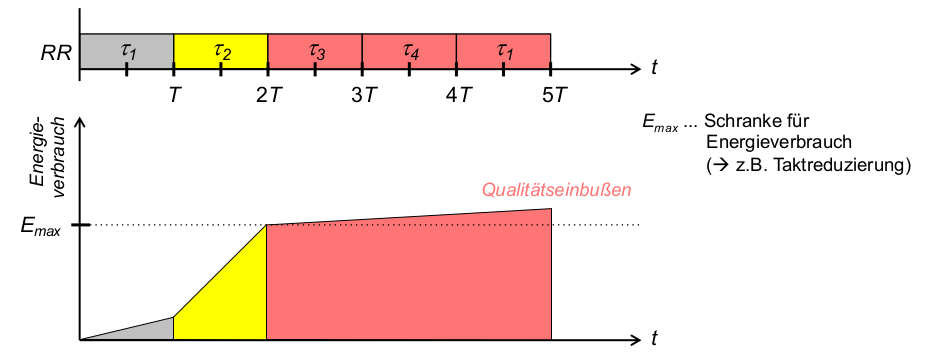
\includegraphics[width=\linewidth]{Assets/AdvancedOperatingSystems-round-robin-unfair.png} \end{itemize*}
            %\end{itemize*}
            \item Problem 2: energieintensive Threads niedrigerer Priorität behindern
            später ankommende Threads höherer Priorität
            %\begin{itemize*}
            %\item \includegraphics[width=\linewidth]{Assets/AdvancedOperatingSystems-prioritätsumkehr.png}
            %\end{itemize*}
        \end{itemize*}
    \end{itemize*}

    Energiebewusstes RR: Fairness

    \begin{itemize*}
        \item
        Begriffe:
        \begin{itemize*}
            \item \$E\_i\^{}\{budget\}\$ ... Energiebudget von \$t\_i\$
            \item \$E\_i\^{}\{limit\}\$ ... Energielimit von \$t\_i\$
            \item \$P\_\{limit\}\$ ... Leistungslimit: maximale Leistungsaufnahme {[}Energie/Zeit{]}
            \item \$T\$ ... resultierende Zeitscheibenlänge
        \end{itemize*}
        \item
        Strategie 1: faire Energieverteilung (einheitliche Energielimits)
        \begin{itemize*}
            %\item
            % %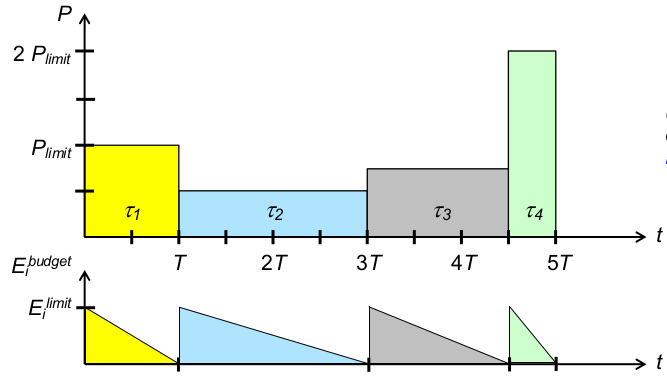
\includegraphics[width=\linewidth]{Assets/AdvancedOperatingSystems-energiebewusstes-rr.png}
            \item \$1\textbackslash leq i\textbackslash leq 4: E\_i\^{}\{limit\} = P\_\{limit\}* T\$
            \item (Abweichungen = Wichtung der Prozesse $\rightarrow$ bedingte Fairness)
        \end{itemize*}
    \end{itemize*}

    Energiebewusstes RR: Reaktivität

    \begin{itemize*}
        \item
        faire bzw. gewichtete Aufteilung begrenzter Energie optimiert
        Energieeffizienz
        \item
        Problem: lange, wenig energieintensive Threads verzögern Antwort-und
        Wartezeiten kurzer, energieintensiver Threads
        \begin{itemize*}
            \item Lösung im Einzelfall: Wichtung per \$E\_i\^{}\{limit\}\$
            \item globale Reaktivität ( $\rightarrow$ Nutzererfahrung bei interaktiven Systemen) ...?
        \end{itemize*}
        \item
        Strategie 2: maximale Reaktivität ( $\rightarrow$
        klassisches RR)
        %\begin{itemize*}
        %\item \includegraphics[width=\linewidth]{Assets/AdvancedOperatingSystems-energiebewusstes-rr-reaktivität.png}
        %\end{itemize*}
    \end{itemize*}

    Energiebewusstes RR: Reaktivität und Fairness

    \begin{itemize*}
        \item
        Problem: sparsame Threads werden bestraft durch Verfallen des
        ungenutzten Energiebudgets
        \item
        Idee: Ansparen von Energiebudgets $\rightarrow$
        mehrfache Ausführung eines Threads innerhalb einer Scheduling-Periode
        \item
        Strategie 3: Reaktivität, dann faire Energieverteilung
        %\begin{itemize*}
        %\item 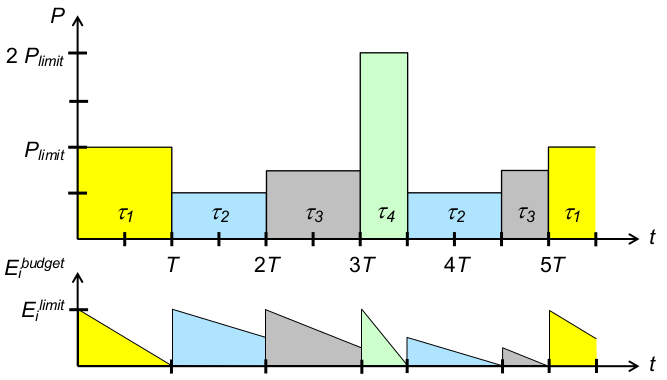
\includegraphics[width=\linewidth]{Assets/AdvancedOperatingSystems-energiebewisstes-rr-2.png}
        %\end{itemize*}
    \end{itemize*}

    \subparagraph{Implementierungsfragen}
    \begin{itemize*}
        \item
        Scheduling-Zeitpunkte?
        \begin{itemize*}
            \item welche Accounting-Operationen (Buchführung über Budget)?
            \item wann Accounting-Operationen?
            \item wann Verdrängung?
        \end{itemize*}
        \item
        Datenstrukturen?
        \begin{itemize*}
            \item ... im Scheduler $\rightarrow$ Warteschlange(n)?
            \item ... im Prozessdeskriptor?
        \end{itemize*}
        \item
        Kosten ggü. klassischem RR? (durch Prioritäten...?)
        \item
        Pro:
        \begin{itemize*}
            \item Optimierung der Energieverteilung nach anwendungsspezifischen Schedulingzielen( $\rightarrow$ Strategien)
            \item Berücksichtigung von prozessspezifischen Energieverbrauchsmustern möglich:fördert Skalierbarkeit i.S.v. Lastadaptivität, indirekt auch Usability ( $\rightarrow$ Nutzererfahrung)
        \end{itemize*}
        \item
        Kontra:
        \begin{itemize*}
            \item zusätzliche sekundäre Kosten: Energiebedarf des Schedulers, Energiebedarf zusätzlicher Kontextwechsel, Implementierungskosten (Rechenzeit, Speicher)
            \item Voraussetzung hardwareseitig: Monitoring des Energieverbrauchs (erforderliche/realisierbare Granularität...? sonst: Extrapolation?)
        \end{itemize*}
        \item
        \textbf{generelle Alternative:} energieintensive Prozesse verlangsamen
        $\rightarrow$ Regelung der CPU-Leistungsparameter
        (Versorgungsspannung) (auch komplementär zum Schedulingals Maßnahme
        nach Energielimit-Überschreitung)
        \item
        Beispiel: Synergie nichtfunktionaler Eigenschaften
        \begin{itemize*}
            \item Performanz nur möglich durch Parallelität $\rightarrow$ Multicore-Hardware
            \item Multicore-Hardware nur möglich mit Lastausgleich und Lastverteilungauf mehrere CPUs
            \item dies erfordert ebenfalls Verteilungsstrategien: ,,Energy-aware Scheduling'' (Linux-Strategie zur Prozessorallokation -nicht zeitlichem Multiplexing!)
        \end{itemize*}
    \end{itemize*}


    \subsubsection{Systemglobale
        Energieeinsparungsmaßnahmen}

    \begin{itemize*}
        \item
        Traditionelle Betriebssysteme: Entwurf so, dass zu jedem Zeitpunkt
        Spitzen-Performanzangestrebt
        \item
        Beobachtungen:
        \begin{itemize*}
            \item viele Anwendungen benötigen keine Spitzen-Performanz
            \item viele Hardware-Komponenten verbringen Zeit in Leerlaufsituationen bzw. in Situationen, wo keine Spitzen-Performanz erforderlich
        \end{itemize*}
        \item
        Konsequenz (besonders für mobile Systeme) :
        \begin{itemize*}
            \item Hardware mit Niedrigenergiezuständen(Prozessoren und Magnetplattenlaufwerke, aber auch DRAM, Netzwerkschnittstellen, Displays, ...)
            \item somit kann Betriebssystem \textbf{Energie-Management} realisieren
        \end{itemize*}
    \end{itemize*}


    \paragraph{Hardwaretechnologien}

    \begin{itemize*}
        \item
        DPM: Dynamic Power Management
        \begin{itemize*}
            \item versetzt leerlaufende/unbenutzte Hardware-Komponenten selektiv in Zustände mit niedrigem Energieverbrauch
            \item Zustandsübergänge durch Power-Manager (in Hardware) gesteuert, dem bestimmte \emph{DPM-} Strategie (Firmware) zugrunde liegt, um gutes Verhältnis zwischen Performanz/Reaktivität und Energieeinsparung zu erzielen
        \end{itemize*}
        \item
        DVS: Dynamic Voltage Scaling
        \begin{itemize*}
            \item effizientes Verfahren zur dynamischen Regulierungvon Taktfrequenz gemeinsammit Versorgungsspannung
            \item Nutzung quadratischer Abhängigkeitder dynamischen Leistung von Versorgungsspannung
            \item Steuerung/Strategien: Softwareunterstützungnotwendig!
        \end{itemize*}
    \end{itemize*}

    Dynamisches Energiemanagement (DPM)- Strategien (Klassen) bestimmt, wann
    und wie lange eine Hardware-Komponente sich in Energiesparmodusbefinden
    sollte

    \begin{itemize*}
        \item
        Greedy: Hardware-Komponente sofort nach Erreichen des Leerlaufs in
        Energiesparmodus, ,,Aufwecken'' durch neue Anforderung
        \item
        Time-out: Energiesparmodus erst nachdem ein definiertes Intervall im
        Leerlauf, ,,Aufwecken'' wie bei Greedy-Strategien
        \item
        Vorhersage: Energiesparmodus sofort nach Erreichen des Leerlaufs, wenn
        Heuristik vorhersagt,dass Kosten gerechtfertigt
        \item
        Stochastisch: Energiesparmodus auf Grundlage eines stochastischen
        Modells
    \end{itemize*}

    Spannungsskalierung (DVS)

    \begin{itemize*}
        \item
        Ziel: Unterstützung von DPM-Strategien durch Maßnahmen auf Ebene von
        Compiler, Betriebssystem und Applikationen:
        \begin{itemize*}
            \item \textbf{Compiler} \begin{itemize*} \item kann Informationen zur Betriebssystem-Unterstützung bezüglich Spannungs-Einstellung in Anwendungs-Code einstreuen, \item damit zur Laufzeit Informationen über jeweilige Arbeitslast verfügbar \end{itemize*}
        \end{itemize*}
        \item
        \textbf{Betriebssystem (prädiktives Energiemanagement)}
        \begin{itemize*}
            \item kann Benutzung verschiedener Ressourcen (Prozessor usw.) beobachten
            \item kann darüber Vorhersagen tätigen
            \item kann notwendigen Performanzbereich bestimmen
        \end{itemize*}
        \item
        \textbf{Anwendungen}
        \begin{itemize*}
            \item können Informationen über jeweils für sie notwendige Performanz liefern
        \end{itemize*}
        \item
        $\rightarrow$ Kombination mit
        energieefizientemScheduling!
    \end{itemize*}


    \subsection{Speichereffizienz}

    \begin{itemize*}
        \item
        ... heißt: Auslastung des verfügbaren Speichers
        \begin{itemize*}
            \item oft implizit: Hauptspeicherauslastung (memoryfootprint)
            \item besonders für kleine/mobile Systeme: Hintergrundspeicherauslastung
        \end{itemize*}
        \item
        Maße zur Konkretisierung:
        \begin{itemize*}
            \item zeitliche Dimension: Maximum vs. Summe genutzten Speichers?
            \item physischer Speicherverwaltung? $\rightarrow$ Belegungsanteil pAR
            \item virtuelle Speicherverwaltung? $\rightarrow$ Belegungsanteil vAR
        \end{itemize*}
        \item
        Konsequenzen für Ressourcenverwaltung durch BS:
        \begin{itemize*}
            \item Taskverwaltung (Accounting, Multiplexing, Fairness, ...)
            \item Programmiermodell, API (besonders: dynamische Speicherreservierung)
            \item Sinnfrage und ggf. Strategien virtueller Speicherverwaltung (VMM)
        \end{itemize*}
        \item
        Konsequenzen für Betriebssystem selbst:
        \begin{itemize*}
            \item minimaler Speicherbedarfdurch Kernel
            \item minimale Speicherverwaltungskosten (durch obige Aufgaben)
        \end{itemize*}
    \end{itemize*}


    \subsubsection{Hauptspeicherauslastung}

    \begin{itemize*}
        \item
        %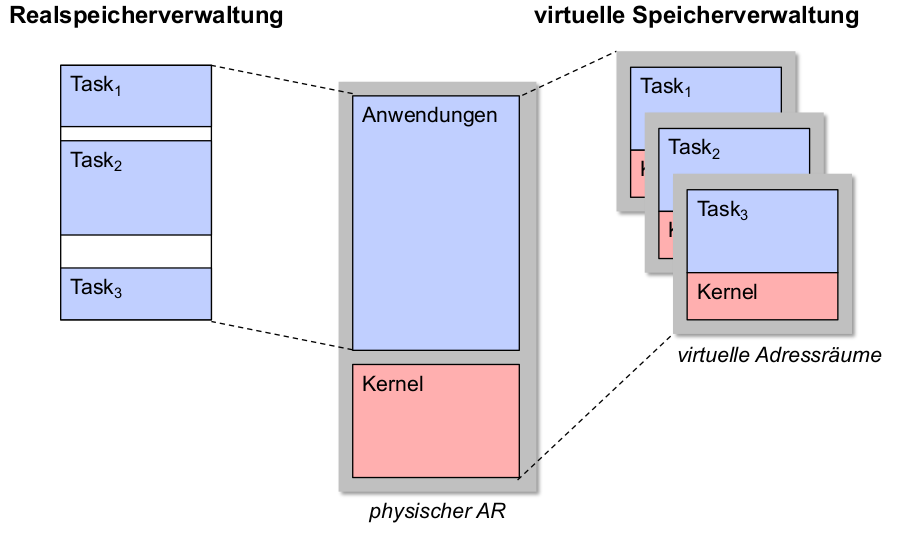
\includegraphics[width=\linewidth]{Assets/AdvancedOperatingSystems-speicherverwaltung.png}
    \end{itemize*}

    Problem: externe Fragmentierung

    \begin{itemize*}
        \item
        %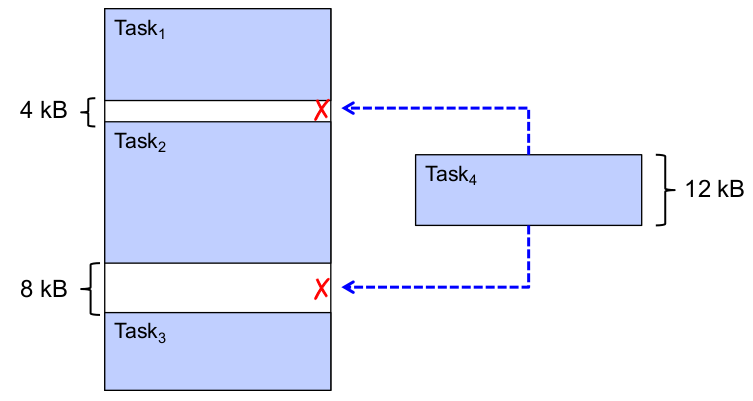
\includegraphics[width=\linewidth]{Assets/AdvancedOperatingSystems-externe-fragmentierung.png}
        \item
        Lösungen:
        \begin{itemize*}
            \item First Fit, Best Fit, WorstFit, Buddy
            \item Relokation
        \end{itemize*}
        \item
        Kompromissloser Weg: kein Multitasking!
    \end{itemize*}

    Problem: interne Fragmentierung

    \begin{itemize*}
        \item
        %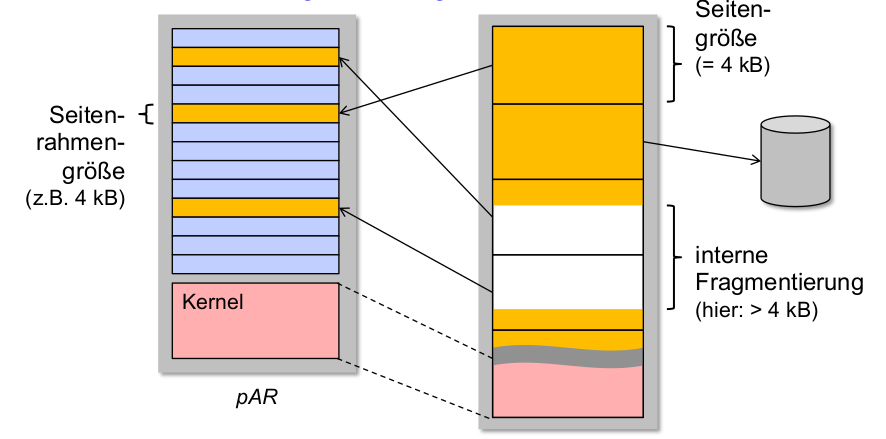
\includegraphics[width=\linewidth]{Assets/AdvancedOperatingSystems-interne-fragmentierung.png}
        \item
        Lösung:
        \begin{itemize*}
            \item Seitenrahmengröße verringern
            \item Tradeoff: dichter belegte vAR $\rightarrow$ größere Datenstrukturen für Seitentabellen!
        \end{itemize*}
        \item
        direkter Einfluss des Betriebssystems auf Hauptspeicherbelegung:
        \begin{itemize*}
            \item $\rightarrow$ Speicherbedarf des Kernels
            \item statische(Minimal-) Größe des Kernels (Anweisungen + Daten)
            \item dynamischeSpeicherreservierung durch Kernel
            \item bei Makrokernel: Speicherbedarf von Gerätecontrollern (Treibern)!
        \end{itemize*}
    \end{itemize*}

    weitere Einflussfaktoren: Speicherverwaltungskosten

    \begin{itemize*}
        \item
        VMM: Seitentabellengröße $\rightarrow$ Mehrstufigkeit
        \item
        Metainformationen über laufende Programme: Größe von
        Taskkontrollblöcken( Prozess-/Threaddeskriptoren ...)
        \item
        dynamische Speicherreservierung durch Tasks
    \end{itemize*}


    \subparagraph{Beispiel 1: sparsam}

    Prozesskontrollblock (PCB, Metadatenstruktur des Prozessdeskriptors)
    eines kleinen Echtzeit-Kernels (,,DICK''):

    %\begin{Shaded}
    %\begin{Highlighting}[]
    %\CommentTok{// Process Control Block (PCB)}
    %\KeywordTok{struct}\NormalTok{ pcb \{}
    % \DataTypeTok{char}\NormalTok{ name[MAXLEN +}\DecValTok{1}\NormalTok{]; }\CommentTok{// process name}
    %\NormalTok{ proc (*addr)(); }\CommentTok{// first instruction}
    % \DataTypeTok{int}\NormalTok{ type; }\CommentTok{// process type}
    % \DataTypeTok{int}\NormalTok{ state; }\CommentTok{// process state}
    % \DataTypeTok{long}\NormalTok{ dline; }\CommentTok{// absolute deadline}
    % \DataTypeTok{int}\NormalTok{ period; }\CommentTok{// period}
    % \DataTypeTok{int}\NormalTok{ prt; }\CommentTok{// priority}
    % \DataTypeTok{int}\NormalTok{ wcet; }\CommentTok{// worst{-}case execution time}
    % \DataTypeTok{float}\NormalTok{ util; }\CommentTok{// processor utilization}
    % \DataTypeTok{int}\NormalTok{ *context;}
    %\NormalTok{ proc next;}
    %\NormalTok{ proc prev;}
    %\NormalTok{\};}
    %\end{Highlighting}
    %\end{Shaded}


    \subparagraph{Beispiel 2: eher nicht sparsam}

    Linux Prozesskontrollblock (taskstruct):

    %\begin{Shaded}
    %\begin{Highlighting}[]
    %\KeywordTok{struct}\NormalTok{ task\_struct \{}
    % \AttributeTok{volatile} \DataTypeTok{long}\NormalTok{ state; }\CommentTok{/* {-} 1 unrunnable, 0 runnable, \textgreater{}0 stopped */}
    % \DataTypeTok{void}\NormalTok{ *stack;}
    % \DataTypeTok{atomic\_t}\NormalTok{ usage;}
    % \DataTypeTok{unsigned} \DataTypeTok{int}\NormalTok{ flags; }\CommentTok{/* per process flags, defined below */}
    % \DataTypeTok{unsigned} \DataTypeTok{int}\NormalTok{ ptrace;}
    %\PreprocessorTok{\#ifdef CONFIG\_SMP}
    % \KeywordTok{struct}\NormalTok{ llist\_node wake\_entry;}
    % \DataTypeTok{int}\NormalTok{ on\_cpu;}
    %\PreprocessorTok{\#endif}
    % \DataTypeTok{int}\NormalTok{ on\_rq;}
    %\CommentTok{// SCHEDULING INFORMATION}
    % \DataTypeTok{int}\NormalTok{ prio, static\_prio, normal\_prio;}
    % \DataTypeTok{unsigned} \DataTypeTok{int}\NormalTok{ rt\_priority;}
    % \AttributeTok{const} \KeywordTok{struct}\NormalTok{ sched\_class *sched\_class;}
    %\CommentTok{// Scheduling Entity}
    % \KeywordTok{struct}\NormalTok{ sched\_entity se;}
    % \KeywordTok{struct}\NormalTok{ sched\_rt\_entity rt;}
    %\PreprocessorTok{\#ifdef CONFIG\_CGROUP\_SCHED}
    % \KeywordTok{struct}\NormalTok{ task\_group *sched\_task\_group;}
    %\PreprocessorTok{\#endif}
    %\PreprocessorTok{\#ifdef CONFIG\_PREEMPT\_NOTIFIERS}
    % \KeywordTok{struct}\NormalTok{ hlist\_head preempt\_notifiers; }\CommentTok{/* list of struct preempt\_notifier */}
    %\PreprocessorTok{\#endif}
    % \DataTypeTok{unsigned} \DataTypeTok{char}\NormalTok{ fpu\_counter;}
    %\PreprocessorTok{\#ifdef CONFIG\_BLK\_DEV\_IO\_TRACE}
    % \DataTypeTok{unsigned} \DataTypeTok{int}\NormalTok{ btrace\_seq;}
    %\PreprocessorTok{\#endif}
    % \DataTypeTok{unsigned} \DataTypeTok{int}\NormalTok{ policy;}
    % \DataTypeTok{cpumask\_t}\NormalTok{ cpus\_allowed;}
    %\PreprocessorTok{\#ifdef CONFIG\_PREEMPT\_RCU}
    % \DataTypeTok{int}\NormalTok{ rcu\_read\_lock\_nesting;}
    % \DataTypeTok{char}\NormalTok{ rcu\_read\_unlock\_special;}
    % \KeywordTok{struct}\NormalTok{ list\_head rcu\_node\_entry;}
    % \KeywordTok{struct}\NormalTok{ rcu\_node *rcu\_blocked\_node;}
    %\PreprocessorTok{\#endif }\CommentTok{/* \#ifdef CONFIG\_TREE\_PREEMPT\_RCU */}
    %\PreprocessorTok{\#ifdef CONFIG\_RCU\_BOOST}
    % \KeywordTok{struct}\NormalTok{ rt\_mutex *rcu\_boost\_mutex;}
    %\PreprocessorTok{\#endif }\CommentTok{/* \#ifdef CONFIG\_RCU\_BOOST */}
    %\PreprocessorTok{\#if defined(CONFIG\_SCHEDSTATS) || defined(CONFIG\_TASK\_DELAY\_ACCT)}
    % \KeywordTok{struct}\NormalTok{ sched\_info sched\_info;}
    %\PreprocessorTok{\#endif}
    % \KeywordTok{struct}\NormalTok{ list\_head tasks;}
    %\PreprocessorTok{\#ifdef CONFIG\_SMP}
    % \KeywordTok{struct}\NormalTok{ plist\_node pushable\_tasks;}
    %\PreprocessorTok{\#endif}
    %\CommentTok{// virtual address space reference}
    % \KeywordTok{struct}\NormalTok{ mm\_struct *mm, *active\_mm;}
    %\PreprocessorTok{\#ifdef CONFIG\_COMPAT\_BRK}
    % \DataTypeTok{unsigned}\NormalTok{ brk\_randomized:}\DecValTok{1}\NormalTok{;}
    %\PreprocessorTok{\#endif}
    %\PreprocessorTok{\#if defined(SPLIT\_RSS\_COUNTING)}
    % \KeywordTok{struct}\NormalTok{ task\_rss\_stat rss\_stat;}
    %\PreprocessorTok{\#endif}
    %\CommentTok{/* task state */}
    % \DataTypeTok{int}\NormalTok{ exit\_state;}
    % \DataTypeTok{int}\NormalTok{ exit\_code, exit\_signal;}
    % \DataTypeTok{int}\NormalTok{ pdeath\_signal; }\CommentTok{/* The signal sent when the parent dies */}
    % \DataTypeTok{unsigned} \DataTypeTok{int}\NormalTok{ jobctl; }\CommentTok{/* JOBCTL\_*, siglock protected */}
    % \DataTypeTok{unsigned} \DataTypeTok{int}\NormalTok{ personality;}
    % \DataTypeTok{unsigned}\NormalTok{ did\_exec:}\DecValTok{1}\NormalTok{;}
    % \DataTypeTok{unsigned}\NormalTok{ in\_execve:}\DecValTok{1}\NormalTok{;}\CommentTok{/* Tell the LSMs that the process is doing an * execve */}
    % \DataTypeTok{unsigned}\NormalTok{ in\_iowait:}\DecValTok{1}\NormalTok{;}
    %\CommentTok{/* Revert to default priority/policy when forking */}
    % \DataTypeTok{unsigned}\NormalTok{ sched\_reset\_on\_fork:}\DecValTok{1}\NormalTok{;}
    % \DataTypeTok{unsigned}\NormalTok{ sched\_contributes\_to\_load:}\DecValTok{1}\NormalTok{;}
    %\PreprocessorTok{\#ifdef CONFIG\_GENERIC\_HARDIRQS}
    %\CommentTok{/* IRQ handler threads */}
    % \DataTypeTok{unsigned}\NormalTok{ irq\_thread;}
    %\PreprocessorTok{\#endif}
    % \DataTypeTok{pid\_t}\NormalTok{ pid;}
    % \DataTypeTok{pid\_t}\NormalTok{ tgid;}
    %\PreprocessorTok{\#ifdef CONFIG\_CC\_STACKPROTECTOR}
    %\CommentTok{/* Canary value for the {-}fstack{-}protector gcc feature */}
    % \DataTypeTok{unsigned} \DataTypeTok{long}\NormalTok{ stack\_canary;}
    %\PreprocessorTok{\#endif}
    %\CommentTok{// Relatives}
    % \KeywordTok{struct}\NormalTok{ task\_struct \_\_rcu *real\_parent; }\CommentTok{/* real parent process */}
    % \KeywordTok{struct}\NormalTok{ task\_struct \_\_rcu *parent; }\CommentTok{/* recipient of SIGCHLD, wait4() reports */}
    %\CommentTok{/* children/sibling forms the list of my natural children */}
    % \KeywordTok{struct}\NormalTok{ list\_head children; }\CommentTok{/* list of my children */}
    % \KeywordTok{struct}\NormalTok{ list\_head sibling; }\CommentTok{/* linkage in my parent\textquotesingle{}s children list */}
    % \KeywordTok{struct}\NormalTok{ task\_struct *group\_leader; }\CommentTok{/* threadgroup leader */}
    % \KeywordTok{struct}\NormalTok{ list\_head ptraced;}
    % \KeywordTok{struct}\NormalTok{ list\_head ptrace\_entry;}
    %\CommentTok{/* PID/PID hash table linkage. */}
    % \KeywordTok{struct}\NormalTok{ pid\_link pids[PIDTYPE\_MAX];}
    % \KeywordTok{struct}\NormalTok{ list\_head thread\_group;}
    % \KeywordTok{struct}\NormalTok{ completion *vfork\_done; }\CommentTok{/* for vfork() */}
    % \DataTypeTok{int}\NormalTok{ \_\_user *set\_child\_tid;}
    %\NormalTok{...}
    % \DataTypeTok{unsigned} \DataTypeTok{long}\NormalTok{ timer\_slack\_ns;}
    % \DataTypeTok{unsigned} \DataTypeTok{long}\NormalTok{ default\_timer\_slack\_ns;}
    % \KeywordTok{struct}\NormalTok{ list\_head *scm\_work\_list;}
    %\PreprocessorTok{\#ifdef CONFIG\_FUNCTION\_GRAPH\_TRACER}
    %\CommentTok{/* Index of current stored address in ret\_stack */}
    % \DataTypeTok{int}\NormalTok{ curr\_ret\_stack;}
    %\CommentTok{/* Stack of return addresses for return function tracing */}
    % \KeywordTok{struct}\NormalTok{ ftrace\_ret\_stack *ret\_stack;}
    %\CommentTok{/* time stamp for last schedule */}
    % \DataTypeTok{unsigned} \DataTypeTok{long} \DataTypeTok{long}\NormalTok{ ftrace\_timestamp;}
    %\NormalTok{...}
    %\end{Highlighting}
    %\end{Shaded}


    \subsubsection{Hintergrundspeicherauslastung}

    Einflussfaktoren des Betriebssystems:

    \begin{itemize*}
        \item
        statische Größe des Kernel-Images, welches beim Bootstrapping gelesen
        wird
        \item
        statische Größe von Programm-Images (Standards wie ELF)
        \item
        statisches vs. dynamisches Einbinden von Bibliotheken: Größe von
        Programmdateien
        \item
        VMM: Größe des Auslagerungsbereichs (inkl. Teilen der Seitentabelle!)
        für Anwendungen
        \item
        Modularisierung (zur Kompilierzeit) des Kernels: gezielte Anpassung an
        Einsatzdomäne möglich
        \item
        Adaptivität (zur Kompilier-und Laufzeit) des Kernels: gezielte
        Anpassung an sich ändernde Umgebungsbedingungen möglich
        ( $\rightarrow$ Cassini-Huygens-Mission)
    \end{itemize*}


    \subsection{Architekturentscheidungen}

    \begin{itemize*}
        \item
        bisher betrachtete Mechanismen: allgemein für alle BS gültig
        \item
        ... typische Einsatzgebiete sparsamer BS: eingebettete Systeme
        \item
        eingebettetes System: (nach {[}Manl94{]} )
        \begin{itemize*}
            \item Computersystem, das in ein größeres technisches System, welches nicht zur Datenverarbeitung dient,physisch eingebunden ist.
            \item Wesentlicher Bestandteil dieses größeren Systems hinsichtlich seiner Entwicklung, technischer Ausstattung sowie seines Betriebs.
            \item Liefert Ausgaben in Form von (menschenlesbaren)Informationen, (maschinenlesbaren)Daten zur Weiterverarbeitung und Steuersignalen.
        \end{itemize*}
        \item
        BS für eingebettete Systeme: spezielle, anwendungsspezifische
        Ausprägung der Aufgaben eines ,,klassischen'' Universal-BS
        \begin{itemize*}
            \item reduzierter Umfang von HW-Abstraktion, generell: hardwarenähere Ablaufumgebung
            \item begrenzte (extrem: gar keine) Notwendigkeit von HW-Multiplexing \& -Schutz
        \end{itemize*}
        \item
        daher eng verwandte NFE: Adaptivitätvon sparsamen BS
        \item
        sparsame Betriebssysteme:
        \begin{itemize*}
            \item energieeffizient \textasciitilde{} geringe Architekturanforderungen an energieintensive Hardware (besonders CPU, MMU, Netzwerk)
            \item speichereffizient \textasciitilde{} Auskommen mit kleinen Datenstrukturen (memory footprint)
        \end{itemize*}
        \item
        Konsequenz: geringe logische Komplexität des Betriebssystemkerns
        \item
        sekundär: Adaptivität des Betriebssystemkerns
    \end{itemize*}


    \subsubsection{Makrokernel (monolithischer
        Kernel)}

    %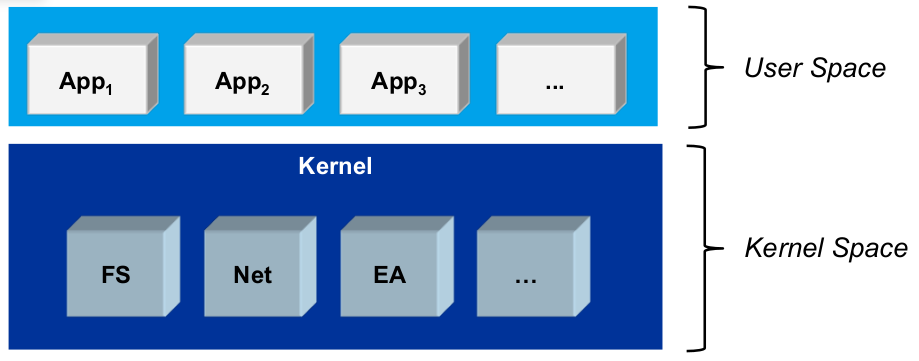
\includegraphics[width=\linewidth]{Assets/AdvancedOperatingSystems-makrokernel.png}

    \begin{itemize*}
        \item
        User Space:
        \begin{itemize*}
            \item Anwendungstasks
            \item CPU im unprivilegiertenModus (Unix ,,Ringe'' 1...3)
            \item Isolation von Tasks durch Programmiermodell(z.B. Namespaces) oder VMM(private vAR)
        \end{itemize*}
        \item
        Kernel Space:
        \begin{itemize*}
            \item Kernelund Gerätecontroller (Treiber)
            \item CPU im privilegierten Modus (Unix ,,Ring'' 0)
            \item keine Isolation (VMM: Kernel wird in alle vAR eingeblendet)
        \end{itemize*}
    \end{itemize*}


    \subsubsection{Mikrokernel}

    %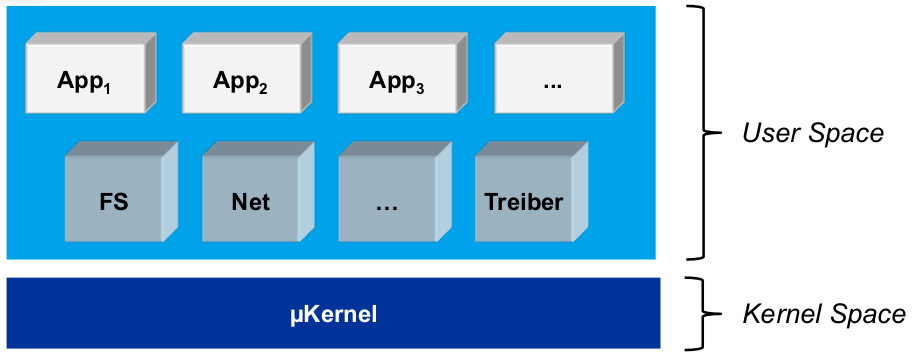
\includegraphics[width=\linewidth]{Assets/AdvancedOperatingSystems-mikrokernel.png}

    \begin{itemize*}
        \item
        User Space:
        \begin{itemize*}
            \item Anwendungstasks, Kernel-und Treiber tasks ( Serverprozesse, grau)
            \item CPU im unprivilegiertenModus
            \item Isolation von Tasks durch VMM
        \end{itemize*}
        \item
        Kernel Space:
        \begin{itemize*}
            \item funktional minimaler Kernel($\mu$Kernel)
            \item CPU im privilegierten Modus
            \item keine Isolation (Kernel wird in alle vAR eingeblendet)
        \end{itemize*}
    \end{itemize*}


    \subsubsection{Architekturkonzepte im
        Vergleich}

    \begin{itemize*}
        \item
        Makrokernel:
        \begin{itemize*}
            \item \cmark vglw. geringe Kosten von Kernelcode (Energie, Speicher)
            \item \cmark VMM nicht zwingend erforderlich
            \item \cmark Multitasking ( $\rightarrow$ Prozessmanagement!)nicht zwingend erforderlich
            \item \xmark Kernel (inkl. Treibern) jederzeit im Speicher
            \item \xmark Robustheit, Sicherheit, Adaptivität
        \end{itemize*}
        \item
        Mikrokernel:
        \begin{itemize*}
            \item \cmark Robustheit, Sicherheit, Adaptivität
            \item \cmark Kernelspeicherbedarf gering, Serverprozesse nur wenn benötigt ( $\rightarrow$ Adaptivität)
            \item \xmark hohe IPC-Kosten von Serverprozessen
            \item \xmark Kontextwechselkosten von Serverprozessen
            \item \xmark VMM, Multitasking i.d.R. erforderlich
        \end{itemize*}
    \end{itemize*}


    \subsection{Beispiel-Betriebssysteme}


    \subsubsection{TinyOS}

    \begin{itemize*}
        \item Beispiel für sparsame BS im Bereich eingebetteter Systeme
        \item verbreitete Anwendung: verteilte Sensornetze (WSN)
        \item ,,TinyOS'' ist ein quelloffenes, BSD-lizenziertes Betriebssystem
        \item das für drahtlose Geräte mit geringem Stromverbrauch, wie sie in
        \begin{itemize*}
            \item Sensornetzwerke, ( $\rightarrow$ Smart Dust)
            \item Allgegenwärtiges Computing,
            \item Personal Area Networks,
            \item intelligente Gebäude,
            \item und intelligente Zähler.
        \end{itemize*}
        \item
        Architektur:
        \begin{itemize*}
            \item grundsätzlich: monolithisch (Makrokernel) mit Besonderheiten:
            \item keine klare Trennung zwischen der Implementierung von Anwendungen und BS (wohl aber von deren funktionalen Aufgaben!)
            \item $\rightarrow$ zur Laufzeit: 1 Anwendung + Kernel
        \end{itemize*}
        \item
        Mechanismen:
        \begin{itemize*}
            \item kein Multithreading, keine echte Parallelität
            \item $\rightarrow$ keine Synchronisation zwischen Tasks
            \item $\rightarrow$ keine Kontextwechsel bei Taskwechsel
            \item Multitasking realisiert durch Programmiermodell
            \item nicht-präemptives FIFO-Scheduling
            \item kein Paging $\rightarrow$ keine Seitentabellen, keine MMU
        \end{itemize*}
        \item
        in Zahlen:
        \begin{itemize*}
            \item Kernelgröße: 400 Byte
            \item Kernelimagegröße: 1 - 4 kByte
            \item Anwendungsgröße: typisch ca. 15 kB, Datenbankanwendung: 64 kB
        \end{itemize*}
        \item
        Programmiermodell:
        \begin{itemize*}
            \item BS und Anwendung werden als Ganzes übersetzt: statische Optimierungen durch Compilermöglich (Laufzeit, Speicherbedarf)
            \item Nebenläufigkeit durch ereignisbasierte Kommunikation zw. Anwendung und Kernel \begin{itemize*} \item $\rightarrow$ command: API-Aufruf, z.B. EA-Operation (vglb. Systemaufruf) \item $\rightarrow$ event: Reaktion auf diesen durch Anwendung \end{itemize*}
            \item sowohl commands als auch events : asynchron
        \end{itemize*}
    \end{itemize*}
    Beispieldeklaration:

    %\begin{Shaded}
    %\begin{Highlighting}[]
    %\NormalTok{interface Timer \{}
    %\NormalTok{ command }\DataTypeTok{result\_t}\NormalTok{ start(}\DataTypeTok{char}\NormalTok{ type, }\DataTypeTok{uint32\_t}\NormalTok{ interval);}
    %\NormalTok{ command }\DataTypeTok{result\_t}\NormalTok{ stop();}
    %\NormalTok{ event }\DataTypeTok{result\_t}\NormalTok{ fired();}
    %%\NormalTok{\}}
    %\NormalTok{interface SendMsg \{}
    %\NormalTok{ command }\DataTypeTok{result\_t}\NormalTok{ send(}\DataTypeTok{uint16\_t}\NormalTok{ address, }\DataTypeTok{uint8\_t}\NormalTok{ length, TOS\_MsgPtr msg);}
    %\NormalTok{ event }\DataTypeTok{result\_t}\NormalTok{ sendDone(TOS\_MsgPtr msg, }\DataTypeTok{result\_t}\NormalTok{ success);}
    %\NormalTok{\}}
    %\end{Highlighting}
    %\end{Shaded}
    %\end{itemize*}


    \subsubsection{RIOT}

    {[}RIOT-Homepage: http://www.riot-os.org{]}

    \begin{itemize*}
        \item
        ebenfalls sparsames BS,optimiert für anspruchsvollere Anwendungen
        (breiteres Spektrum)
        \item
        ,,RIOT ist ein Open-Source-Mikrokernel-basiertes Betriebssystem, das
        speziell für die Anforderungen von Internet-of-Things-Geräten (IoT)
        und anderen eingebetteten Geräten entwickelt wurde.''
        \begin{itemize*}
            \item Smartdevices,
            \item intelligentes Zuhause, intelligente Zähler,
            \item eingebettete Unterhaltungssysteme
            \item persönliche Gesundheitsgeräte,
            \item intelligentes Fahren,
            \item Geräte zur Verfolgung und Überwachung der Logistik.
        \end{itemize*}
        \item
        Architektur:
        \begin{itemize*}
            \item halbwegs: Mikrokernel
            \item energiesparendeKernelfunktionalität:
            \begin{itemize*}
                \item minimale Algorithmenkomplexität
                \item vereinfachtes Threadkonzept $\rightarrow$ keine Kontextsicherung erforderlich
                \item keine dynamische Speicherallokation
                \item energiesparende Hardwarezustände vom Scheduler ausgelöst (inaktive CPU)
            \end{itemize*}
            \item Mikrokerneldesign unterstützt komplementäre NFE: Adaptivität, Erweiterbarkeit
            \item Kosten: IPC (hier gering!)
        \end{itemize*}
        \item
        Mechanismen:
        \begin{itemize*}
            \item Multithreading-Programmiermodell
            \item modulare Implementierung von Dateisystemen, Scheduler, Netzwerkstack
        \end{itemize*}
        \item
        in Zahlen:
        \begin{itemize*}
            \item Kernelgröße: 1,5 kByte
            \item Kernelimagegröße: 5 kByte
        \end{itemize*}
    \end{itemize*}

    Implementierung

    \begin{itemize*}
        \item
        ... kann sich jeder mal ansehen (keine spezielle Hardware, beliebige
        Linux-Distribution, FreeBSD, macOSX mit git ):

        %\begin{Shaded}
        %\begin{Highlighting}[]
        %\NormalTok{$ }\FunctionTok{git}\NormalTok{ clone git://github.com/RIOT{-}OS/RIOT.git}
        %\NormalTok{$ }\BuiltInTok{cd}\NormalTok{ RIOT}
        %\NormalTok{$ }\BuiltInTok{cd}\NormalTok{ examples/default/}
        %\NormalTok{$ }\FunctionTok{make}\NormalTok{ all}
        %\NormalTok{$ }\FunctionTok{make}\NormalTok{ term}
        %\end{Highlighting}
        %\end{Shaded}
        \item
        startet interaktive Instanz von RIOT als ein Prozess des Host-BS
        \item
        Verzeichnis RIOT: Quellenzur Kompilierung des Kernels, mitgelieferte
        Bibliotheken, Gerätetreiber, Beispielanwendungen; z.B.:
        \begin{itemize*}
            \item RIOT/core/include/thread.h: Threadmodell, Threaddeskriptor
            \item RIOT/core/include/sched.h,
            \item RIOT/core/sched.c: Implementierung des (einfachen) Schedulers
        \end{itemize*}
        \item
        weitere Infos: riot-os.org/api
    \end{itemize*}


    \section{Robustheit und
      Verfügbarkeit}


    \subsection{Motivation}

    \begin{itemize*}
        \item
        allgemein: verlässlichkeitskritischeAnwendungsszenarien
        \item
        Forschung in garstiger Umwelt
        \item
        Weltraumerkundung
        \item
        hochsicherheitskritische Systeme:
        \begin{itemize*}
            \item Rechenzentren von Finanzdienstleistern
            \item Rechenzentren von Cloud-Dienstleistern
        \end{itemize*}
        \item
        hochverfügbare System:
        \begin{itemize*}
            \item all das bereits genannte
            \item öffentliche Infrastruktur(Strom, Fernwärme, ...)
        \end{itemize*}
        \item
        HPC (high performancecomputing)
    \end{itemize*}


    \subsection{Allgemeine Begriffe}

    \begin{itemize*}
        \item
        Verlässlichkeit, Zuverlässigkeit (dependability)
        \item
        übergeordnete Eigenschaft eines Systems {[}ALRL04{]}
        \item
        Fähigkeit, eine Leistungzu erbringen, der man berechtigterweise
        vertrauen kann
        \item
        Taxonomie: umfasst entsprechend Definition die Untereigenschaften
        \begin{enumerate*}

            \item Verfügbarkeit (availability)
            \item Robustheit (robustness, reliability
            \item (Funktions-) Sicherheit (safety)
            \item Vertraulichkeit (confidentiality)
            \item Integrität (integrity)
            \item Wartbarkeit (maintainability) (vgl.: evolutionäre Eigenschaften)
        \end{enumerate*}
        \item
        1., 4. \& 5. auch Untereigenschaften von IT-Sicherheit (security)
        \item
        $\rightarrow$ nicht für alle Anwendungen sind alle
        Untereigenschaften erforderlich
    \end{itemize*}


    \subsubsection{Robustheitsbegriff}

    \begin{itemize*}
        \item
        Teil der primären Untereigenschaften von Verlässlichkeit: Robustheit
        (robustness, reliability)
        \item
        Ausfall: beobachtbare Verminderung der Leistung, die ein System
        tatsächlich erbringt, gegenüber seiner als korrekt spezifizierten
        Leistung
        \item
        Robustheit: Verlässlichkeit unter Anwesenheit externer Ausfälle (=
        Ausfälle, deren Ursache außerhalb des betrachteten Systems liegt)
        \item
        im Folgenden: kurze Systematik der Ausfälle ...
    \end{itemize*}


    \subsubsection{Fehler und Ausfälle ...}

    \begin{itemize*}
        \item
        Fehler $\rightarrow$ fehlerhafter Zustand
        $\rightarrow$ Ausfall
        \item
        grundlegende Definitionen dieser Begriffe (ausführlich: {[}ALRL04,
        AvLR04{]} ):
        \begin{itemize*}
            \item Ausfall (failure): liegt vor, wenn tatsächliche Leistung(en), die ein System erbringt, von als korrekt spezifizierter Leistung abweichen
            \item fehlerhafter Zustand ( error ): notwendige Ursacheeines Ausfalls (nicht jeder error muss zu failure führen)
            \item Fehler ( fault ): Ursache für fehlerhaften Systemzustand ( error ), z.B. Programmierfehler
        \end{itemize*}
        \item
        %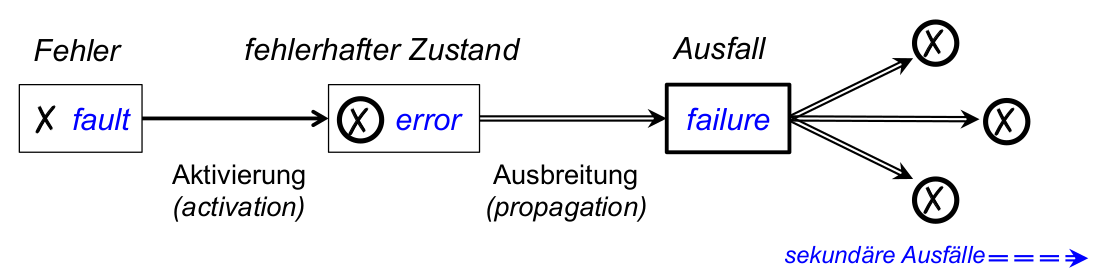
\includegraphics[width=\linewidth]{Assets/AdvancedOperatingSystems-fehler.png}
    \end{itemize*}


    \subsubsection{... und ihre Vermeidung}

    \begin{itemize*}
        \item
        Umgang mit ...
        \begin{itemize*}
            \item faults: \begin{itemize*} \item Korrektheit testen \item Korrektheit beweisen( $\rightarrow$ formale Verifikation) \end{itemize*}
            \item errors: \begin{itemize*} \item Maskierung, Redundanz \item Isolationvon Subsystemen \item $\rightarrow$ Isolationsmechanismen \end{itemize*}
            \item failures: \begin{itemize*} \item Ausfallverhalten (neben korrektem Verhalten) spezifizieren \item Ausfälle zur Laufzeit erkennen und Folgen beheben, abschwächen... \item $\rightarrow$ Micro-Reboots \end{itemize*}
        \end{itemize*}
    \end{itemize*}


    \subsection{Fehlerhafter Zustand}

    \begin{itemize*}
        \item
        interner und externer Zustand (internal \& external state)
        \begin{itemize*}
            \item externer Zustand (einer Systems oder Subsystems): der Teil des Gesamtzustands, der an externer Schnittstelle (also für das umgebende (Sub-) System) sichtbar wird
            \item interner Zustand: restlicher Teilzustand
            \item (tatsächlich) erbrachte Leistung: zeitliche Folge externer Zustände
        \end{itemize*}
        \item
        Beispiele für das System ( Betriebssystem-) Kernel :
        \begin{itemize*}
            \item Subsysteme: Dateisystem, Scheduler, E/A, IPC, ..., Gerätetreiber
            \item fault : Programmierfehler im Gerätetreiber
            \item externer Zustand des Treibers (oder des Dateisystems, Schedulers, E/A, IPC, ...) $\subseteq$ interner Zustand des Kernels
            %\item
            % %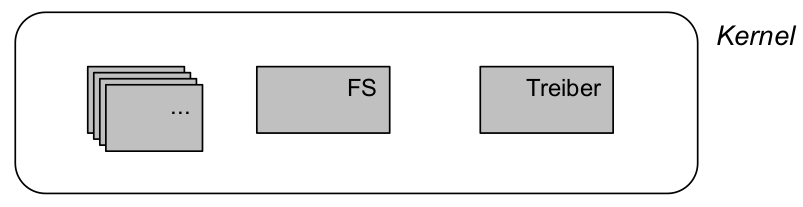
\includegraphics[width=\linewidth]{Assets/AdvancedOperatingSystems-treiber-kernel.png}
        \end{itemize*}
    \end{itemize*}


    \subsubsection{Fehlerausbreitung und (externer)
        Ausfall}

    \begin{itemize*}
        \item
        Wirkungskette: -{[}X{]} Treiber-Programmierfehler (fault) -{[}X{]}
        fehlerhafter interner Zustand des Treibers (error)
        \begin{itemize*}
            \item Ausbreitung dieses Fehlers ( failure des Treibers)
            \item = fehlerhafter externer Zustand des Treibers
            \item = fehlerhafter interner Zustand des Kernels( error )
            \item = Kernelausfall!( failure )
        \end{itemize*}
        \item[$\boxtimes$]
        Auswirkung: fehlerhafter interner Zustand eines weiteren
        Kernel-Subsystems (z.B. error des Dateisystems)
        \item
        $\rightarrow$ Robustheit: Isolationsmechanismen
        \item
        %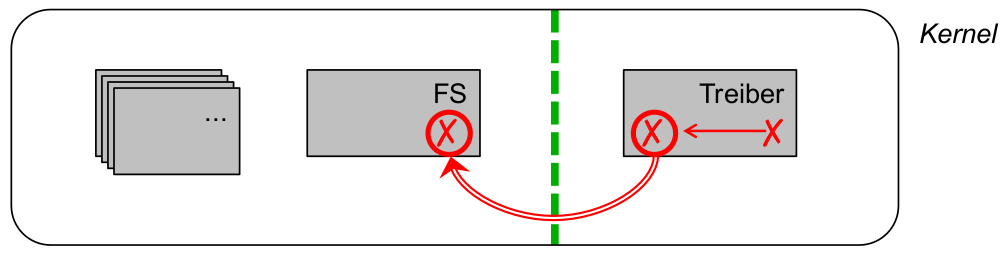
\includegraphics[width=\linewidth]{Assets/AdvancedOperatingSystems-treiber-kernel-fehler.png}
    \end{itemize*}


    \subsection{Isolationsmechanismen}

    \begin{itemize*}
        \item
        im Folgenden: Isolationsmechanismen für robuste Betriebssysteme
        \begin{itemize*}
            \item durch strukturierte Programmierung
            \item durch Adressraumisolation
        \end{itemize*}
        \item
        es gibt noch mehr: Isolationsmechanismen für sichere Betriebssysteme
        \begin{itemize*}
            \item all die obigen...
            \item durch kryptografische Hardwareunterstützung: Enclaves
            \item durch streng typisierte Sprachen und managed code
            \item durch isolierte Laufzeitumgebungen: Virtualisierung
        \end{itemize*}
    \end{itemize*}


    \subsubsection{Strukturierte
        Programmierung}

    Monolithisches BS... in historischer Reinform:

    \begin{itemize*}
        \item
        Anwendungen
        \item
        Kernel
        \item
        gesamte BS-Funktionalität
        \item
        programmiert als Sammlung von Prozeduren
        \item
        jede darf jede davon aufrufen
        \item
        keine Modularisierung
        \item
        keine definierten internen Schnittstellen
    \end{itemize*}


    \paragraph{Monolithisches Prinzip}

    \begin{itemize*}
        \item
        Ziel: Isolation zwischen Anwendungen und Betriebssystem
        \item
        Mechanismus: Prozessor-Privilegierungsebenen ( user space und kernel
        space )
        \item
        Konsequenz für Strukturierung des Kernels: Es gibt keine
        Strukturierung des Kernels ...
        \item
        ... jedenfalls fast: Ablauf eines Systemaufrufs (Erinnerung)
        %\begin{itemize*}
        %\item \includegraphics[width=\linewidth]{Assets/AdvancedOperatingSystems-systemaufruf.png}
        %\end{itemize*}
    \end{itemize*}


    \paragraph{Strukturierte
        Makrokernarchitektur}

    \begin{itemize*}
        \item
        Resultat: schwach strukturierter (monolithischer) Makrokernel
        \item
        %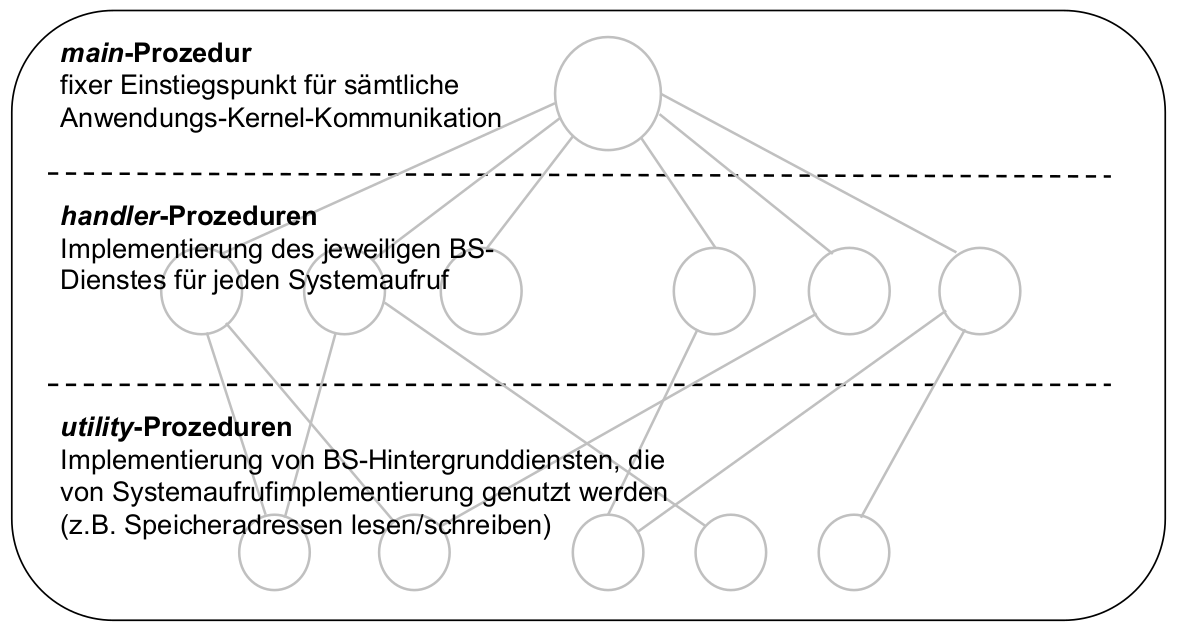
\includegraphics[width=\linewidth]{Assets/AdvancedOperatingSystems-makrokernelarchitektur.png}
        \begin{itemize*}
            \item nach {[}TaWo05{]}, S. 45
        \end{itemize*}
        \item
        Weiterentwicklung:
        \item
        Schichtendifferenzierung ( layered operating system )
        \item
        Modularisierung (Bsp.: Linux-Kernel) \textbar{} Kernelcode \textbar{}
        \textbar{}
        -\/-\/-\/-\/-\/-\/-\/-\/-\/-\/-\/-\/-\/-\/-\/-\/-\/-\/-\/-\/-\/-\/-\/-\/-
        \textbar{} \textbar{} VFS \textbar{} \textbar{} IPC, Dateisystem
        \textbar{} \textbar{} Scheduler, VMM \textbar{} \textbar{} Dispatcher,
        Gerätetreiber \textbar{}
        \item
        Modularer Makrokernel:
        \item
        alle Kernelfunktionen in Moduleunterteilt (z.B. verschiedene
        Dateisystemtypen) $\rightarrow$ Erweiterbarkeit,
        Wartbarkeit, Portierbarkeit
        \item
        klar definierte Modulschnittstellen(z.B. virtualfilesystem, VFS )
        \item
        Module zur Kernellaufzeit dynamisch einbindbar
        ( $\rightarrow$ Adaptivität)
    \end{itemize*}


    \paragraph{Fehlerausbreitung beim
        Makrokernel}

    \begin{itemize*}
        \item
        strukturierte Programmierung:
        \item
        \cmark Wartbarkeit
        \item
        \cmark Portierbarkeit
        \item
        \cmark Erweiterbarkeit
        \item
        O (begrenzt) Adaptivität
        \item
        O (begrenzt) Schutz gegen statische Programmierfehler: nur durch
        Compiler (z.B. C private, public)
        \item
        \xmark kein Schutz gegen dynamische Fehler
        \item
        $\rightarrow$ Robustheit...?
        \item
        nächstes Ziel: Schutz gegen Laufzeitfehler...
        $\rightarrow$ Laufzeitmechanismen
    \end{itemize*}


    \subsubsection{Adressraumisolation}

    \begin{itemize*}
        \item
        zur Erinnerung: private virtuelle Adressräume zweier Tasks
        (\$i\textbackslash not= j\$)
        %\begin{itemize*}
        %\item \includegraphics[width=\linewidth]{Assets/AdvancedOperatingSystems-private-virtuelle-adressräume.png}
        %\end{itemize*}
        \item
        private virtuelle vs. physischer Adresse
        %\begin{itemize*}
        %\item 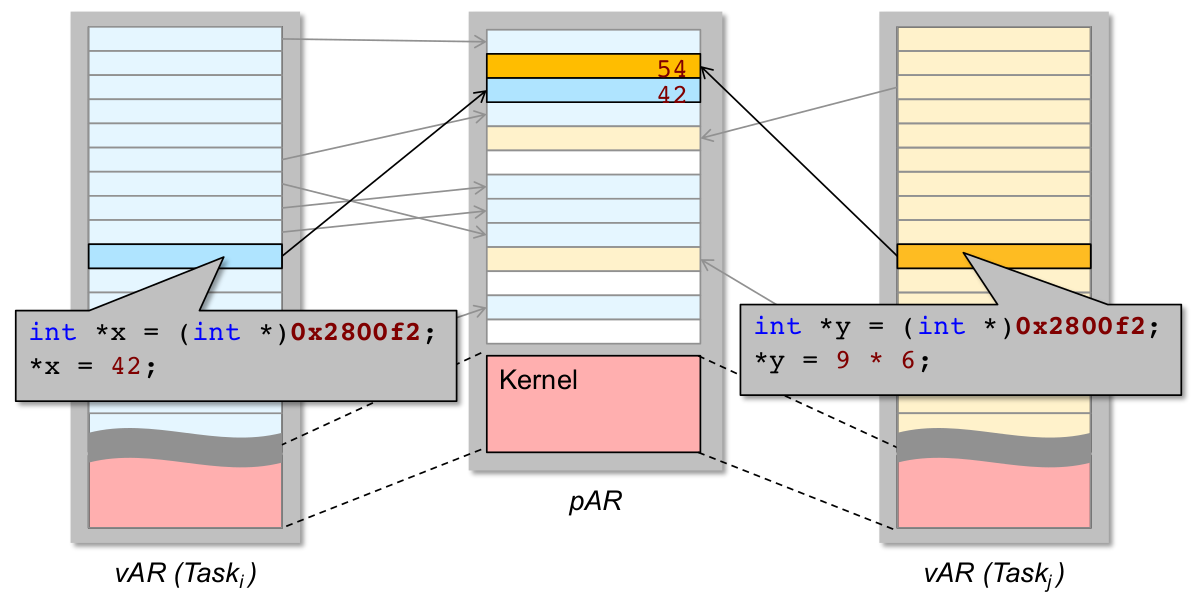
\includegraphics[width=\linewidth]{Assets/AdvancedOperatingSystems-virtuelle-vs-physische-adresse.png}
        %\end{itemize*}
    \end{itemize*}


    \paragraph{Private virtuelle Adressräume und
        Fehlerausbreitung}

    \begin{itemize*}
        \item
        korrekte private vAR \textasciitilde{} kollisionsfreie
        Seitenabbildung!
        \item
        Magie in Hardware: MMU (BS steuert und verwaltet...)
        \item
        Robustheit: Was haben wir von privaten vAR?
        \begin{itemize*}
            \item \cmark nichtvertrauenswürdiger (i.S.v. potenziell nicht korrekter) Code kann keine beliebigen physischen Adressen schreiben (er erreicht sie ja nicht mal...)
            \item \cmark Kommunikation zwischen nvw. Code (z.B. Anwendungstasks) muss durch IPC-Mechanismen explizit hergestellt werden (u.U. auch shared memory) \begin{itemize*} \item $\rightarrow$ Überwachung und Validierung zur Laufzeit möglich \end{itemize*}
            \item \cmark Kontrollfluss begrenzen: Funktionsaufrufe können i.A. (Ausnahme: RPC) keine AR-Grenzen überschreiten \begin{itemize*} \item $\rightarrow$ BS-Zugriffssteuerungkann nicht durch Taskfehler ausgehebelt werden \item $\rightarrow$ unabsichtliche Terminierungsfehler(unendliche Rekursion) erschwert ... \end{itemize*}
        \end{itemize*}
    \end{itemize*}


    \paragraph{Was das für den Kernel
        bedeutet}

    \begin{itemize*}
        \item
        private virtuelle Adressräume
        \begin{itemize*}
            \item gibt es schon so lange wie VMM
            \item gab es lange nur auf Anwendungsebene
            \item $\rightarrow$ keine Isolation zwischen Fehlern innerhalb des Kernels!
            %\item
            % %\includegraphics[width=\linewidth]{Assets/AdvancedOperatingSystems-virtuelle-kernel-adressräume.png}
        \end{itemize*}
        \item
        nächstes Ziel: Schutz gegen Kernelfehler (Gerätetreiber)...
        $\rightarrow$ BS-Architektur
    \end{itemize*}


    \subsection{Mikrokernelarchitektur}

    \begin{itemize*}
        \item Fortschritt ggü. Makrokernel:
        \begin{itemize*}
            \item Strukturierungskonzept:
            \begin{itemize*}
                \item strenger durchgesetzt durch konsequente Isolation voneinander unabhängiger Kernel-Subsysteme
                \item zur Laufzeit durchgesetzt $\rightarrow$ Reaktion auf fehlerhafte Zustände möglich!
            \end{itemize*}
            \item zusätzlich zu vertikaler Strukturierung des Kernels: horizontale Strukturierungeingeführt
            \begin{itemize*}
                \item $\rightarrow$ funktionale Einheiten: vertikal (Schichten)
                \item $\rightarrow$ isolierteEinheiten: horizontal (private vAR)
            \end{itemize*}
        \end{itemize*}
        \item
        Idee:
        \begin{itemize*}
            \item Kernel (alle BS-Funktionalität) $\rightarrow$ $\mu$Kernel (minimale BS-Funktionalität)
            \item Rest (insbes. Treiber): ,,gewöhnliche'' Anwendungsprozesse mit Adressraumisolation
            \item Kommunikation: botschaftenbasierteIPC (auch client-server operating system )
            \item Nomenklatur: Mikrokernelund Serverprozesse
        \end{itemize*}
    \end{itemize*}


    \subsubsection{Modularer Makrokernel vs.
        Mikrokernel}

    \begin{itemize*}
        \item
        %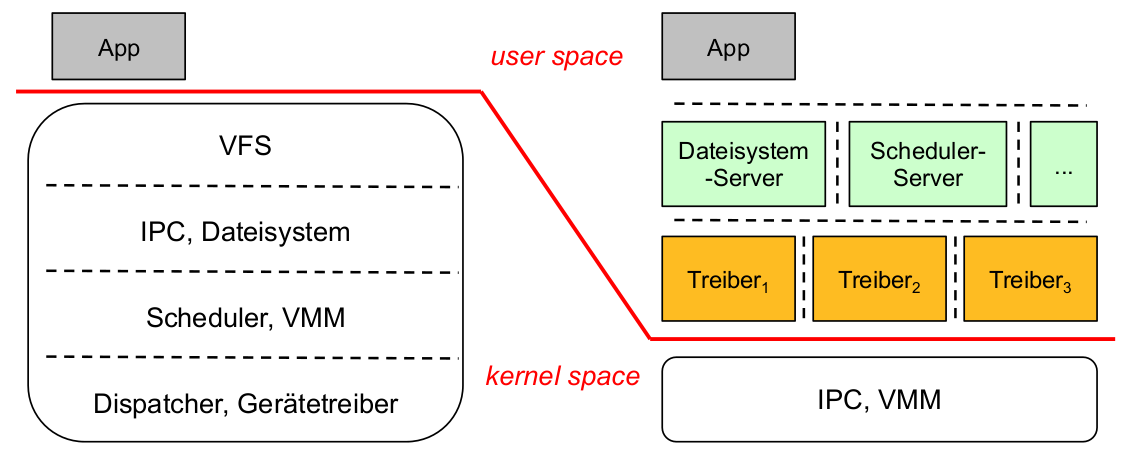
\includegraphics[width=\linewidth]{Assets/AdvancedOperatingSystems-modularer-makrokernel.png}
        \item
        minimale Kernelfunktionalität:
        \item
        keine Dienste, nur allgemeine Schnittstellenfür diese
        \item
        keine Strategien, nur grundlegende Mechanismenzur Ressourcenverwaltung
        \item
        neues Problem: minimales Mikrokerneldesign
        \item
        ,,Wir haben 100 Leute gefragt...'': Wie entscheide ich das?
        \item
        %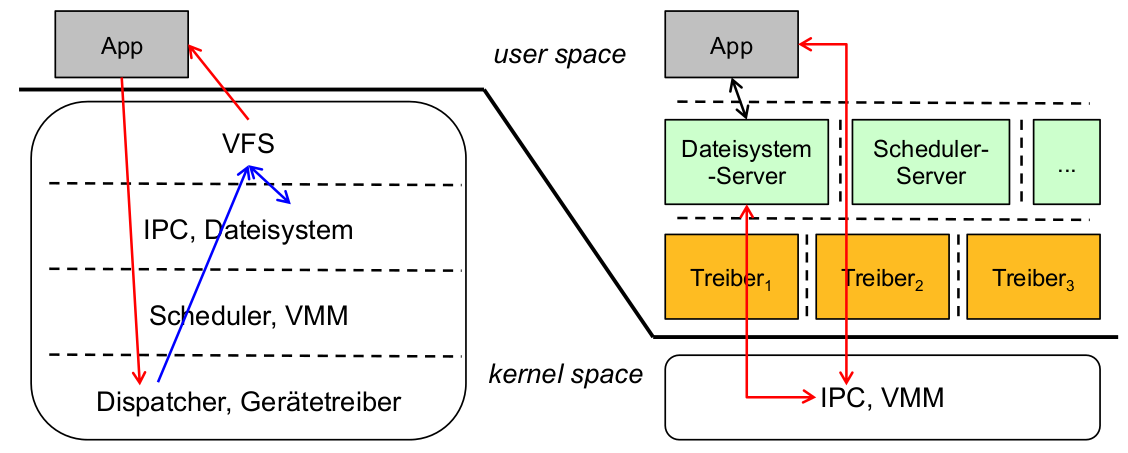
\includegraphics[width=\linewidth]{Assets/AdvancedOperatingSystems-modularer-makrokernel-2.png}
        \begin{itemize*}
            \item Ablauf eines Systemaufrufs
            \item schwarz: unprivilegierteInstruktionen
            \item blau:privilegierte Instruktionen
            \item rot:Übergang zwischen beidem ($\mu$Kern $\rightarrow$ Kontextwechsel!)
        \end{itemize*}
    \end{itemize*}


    \paragraph{Robustheit von
        Mikrokernen}

    \begin{itemize*}
        \item
        = Gewinn durch Adressraumisolation innerhalb des Kernels
        \begin{itemize*}
            \item \cmark kein nichtvertrauenswürdiger Code im kernelspace , der dort beliebige physische Adressen manipulieren kann
            \item \cmark Kommunikation zwischen nvw. Code (nicht zur zwischen Anwendungstasks)muss durch IPC explizit hergestellt werden $\rightarrow$ Überwachung und Validierung zur Laufzeit
            \item \cmark Kontrollfluss begrenzen: Zugriffssteuerung auch zwischen Serverprozessen, zur Laufzeit unabhängiges Teilmanagement von Code (Kernelcode) möglich (z.B.: Nichtterminierung erkennen)
        \end{itemize*}
        \item
        Neu:
        \begin{itemize*}
            \item \cmark nvw. BS-Code muss nicht mehr im kernelspace (höchste Prozessorprivilegierung) laufen
            \item \cmark verbleibender Kernel (dessen Korrektheit wir annehmen): klein, funktional weniger komplex, leichter zu entwickeln, zu testen, evtl. formal zu verifizieren
            \item \cmark daneben: Adaptivitätdurch konsequentere Modularisierung des Kernels gesteigert
        \end{itemize*}
    \end{itemize*}


    \subsubsection{Mach}

    \begin{itemize*}
        \item
        Mikrokernel-Design: Erster Versuch
        \begin{itemize*}
            \item Carnegie Mellon University (CMU), School of Computer Science 1985 - 1994
        \end{itemize*}
        \item
        ein wenig Historie
        \begin{itemize*}
            \item UNIX (Bell Labs) - K. Thompson, D. Ritchie
            \item BSD (U Berkeley) - W. Joy
            \item System V - W. Joy
            \item Mach (CMU) - R. Rashid
            \item MINIX - A. Tanenbaum
            \item NeXTSTEP (NeXT) - S. Jobs
            \item Linux - L. Torvalds
            \item GNU Hurd (FSF) - R. Stallman
            \item Mac OS X (Apple) - S. Jobs
        \end{itemize*}
    \end{itemize*}


    \paragraph{Mach: Ziele}

    Entstehung

    \begin{itemize*}
        \item
        Grundlage:
        \begin{itemize*}
            \item 1975: Aleph(BS des ,,Rochester Intelligent Gateway''), U Rochester
            \item 1979/81: Accent (verteiltes BS), CMU
        \end{itemize*}
        \item
        gefördert durch militärische Geldgeber:
        \begin{itemize*}
            \item DARPA: Defense AdvancedResearch Projects Agency
            \item SCI: Strategic Computing Initiative
        \end{itemize*}
    \end{itemize*}

    Ziele

    \begin{itemize*}
        \item
        Mach 3.0 (Richard Rashid, 1989): einer der ersten praktisch nutzbaren
        $\mu$Kerne
        \item
        Ziel: API-Emulation($\not =$ Virtualisierung!)von UNIX und -Derivaten auf
        unterschiedlichen Prozessorarchitekturen
        \item
        mehrere unterschiedliche Emulatoren gleichzeitig lauffähig
        \begin{itemize*}
            \item Emulation außerhalb des Kernels
            \item jeder Emulator: \begin{itemize*} \item Komponente im Adressraum des Applikationsprogramms \item 1...n Server, die unabhängig von Applikationsprogramm laufen \end{itemize*}
        \end{itemize*}
    \end{itemize*}

    Mach-Server zur Emulation

    \begin{itemize*}
        \item
        %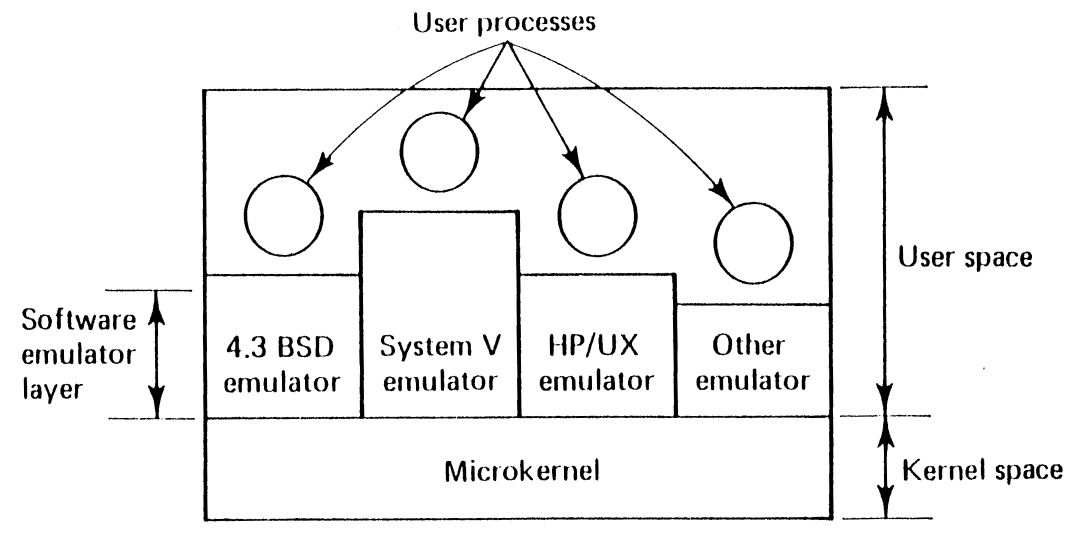
\includegraphics[width=\linewidth]{Assets/AdvancedOperatingSystems-mach-server.png}
        \item
        Emulation von UNIX-Systemen mittels Mach-Serverprozessen
    \end{itemize*}

    $\mu$Kernel-Funktionen

    \begin{enumerate*}
        \item
        Prozessverwaltung
        \item
        Speicherverwaltung
        \item
        IPC-und E/A-Dienste, einschließlich Gerätetreiber
    \end{enumerate*}

    unterstützte Abstraktionen ( $\rightarrow$ API,
    Systemaufrufe):

    \begin{enumerate*}
        \item
        Prozesse
        \item
        Threads
        \item
        Speicherobjekte
        \item
        Ports (generisches, ortstransparentes Adressierungskonzept; vgl. UNIX
        ,,everything is a file'')
        \item
        Botschaften
        \item
        ... (sekundäre, von den obigen genutzte Abstraktionen)
    \end{enumerate*}

    Architektur

    \begin{itemize*}
        \item
        %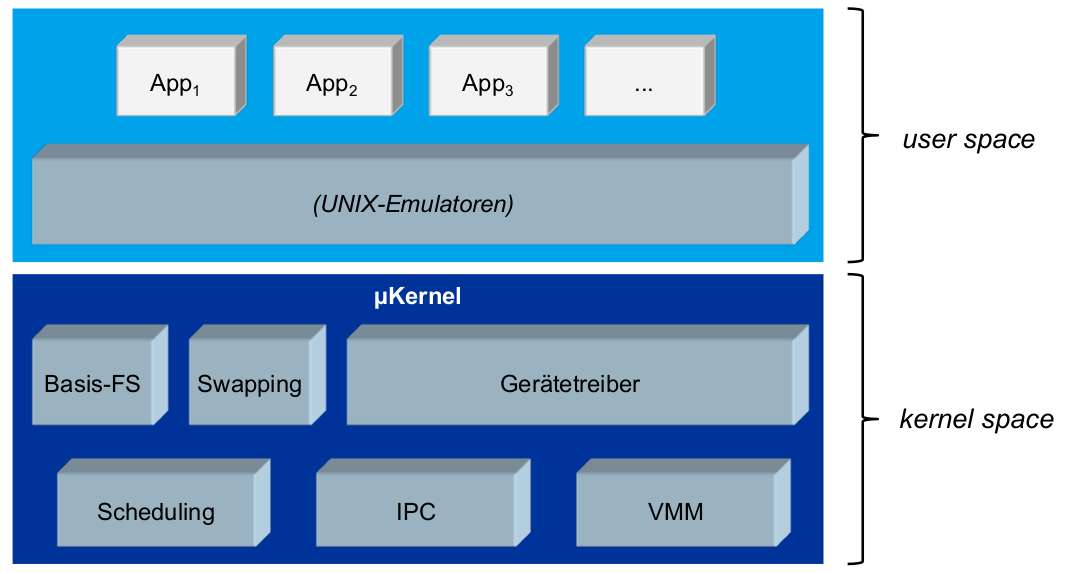
\includegraphics[width=\linewidth]{Assets/AdvancedOperatingSystems-mach-architektur.png}
        \item
        Systemaufrufkosten:
        \begin{itemize*}
            \item IPC-Benchmark (1995): i486 Prozessor, 50 MHz
            \item Messung mit verschiedenen Botschaftenlängen( x - Werte)
            \item ohne Nutzdaten (0 Byte Botschaftenlänge): 115 $\mu$s (Tendenz unfreundlich ...)
            %\item
            % %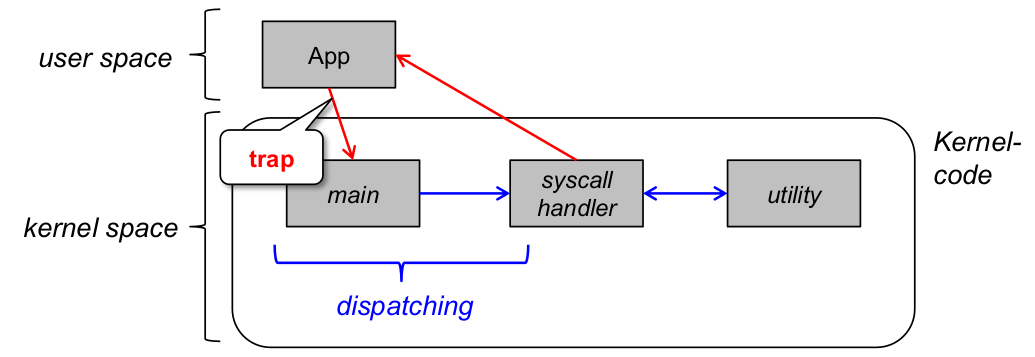
\includegraphics[width=\linewidth]{Assets/AdvancedOperatingSystems-mach-systemaufruf.png}
        \end{itemize*}
        \item
        Bewertung aus heutiger Sicht:
        \begin{itemize*}
            \item funktional komplex
            \item 153 Systemaufrufe
            \item mehrere Schnittstellen, parallele Implementierungen für eine Funktion
            \item $\rightarrow$ Adaptivität (Auswahl durch Programmierer)
        \end{itemize*}
        \item
        Fazit:
        \begin{itemize*}
            \item zukunftsweisender Ansatz
            \item langsame und ineffiziente Implementierung
        \end{itemize*}
    \end{itemize*}

    Lessons Learned

    \begin{itemize*}
        \item
        erster Versuch:
        \item
        Idee des Mikrokernelsbekannt
        \item
        Umsetzung: Designkriterienweitgehend unbekannt
        \item
        Folgen für Performanz und Programmierkomfort: {[}Heis19{]}
        \item
        \xmark ,,complex''
        \item
        \xmark ,,inflexible''
        \item
        \xmark ,,slow''
        \item
        wir wissen etwas über Kosten: IPC-Performanz, Kernelabstraktionen
        \item
        wir wissen noch nichts über guten $\mu$Kern-Funktionsumfangund gute
        Schnittstellen...
        \item
        $\rightarrow$ nächstes Ziel!
    \end{itemize*}


    \subsubsection{L4}

    \begin{itemize*}
        \item
        Made in Germany:
        \begin{itemize*}
            \item Jochen Liedtke (GMD, ,,Gesellschaft für Mathematik und Datenverarbeitung''), Betriebssystemgruppe (u.a.): J. Liedtke, H. Härtig, W. E. Kühnhauser
            \item Symposium on Operating Systems Principles 1995 (SOSP '95): ,,On $\mu$-Kernel Construction'' {[}Lied95{]}
        \end{itemize*}
        \item
        Analyse des Mach-Kernels:
        \begin{enumerate*}

            \item falsche Abstraktionen
            \item unperformanteKernelimplementierung
            \item prozessorunabhängige Implementierung \begin{itemize*} \item Letzteres: effizienzschädliche Eigenschaft eines Mikrokernels \item Neuimplementierung eines (konzeptionell sauberen!) $\mu$-Kerns kaum teurer als Portierung auf andere Prozessorarchitektur \end{itemize*}
        \end{enumerate*}
    \end{itemize*}

    L3 und L4

    \begin{itemize*}
        \item
        Mikrokerne der 2. Generation
        \item
        zunächst L3, insbesondere Nachfolger L4: erste Mikrokerne der 2.
        Generation
        \item
        vollständige Überarbeitung des Mikrokernkonzepts: wesentliche Probleme
        der 1. Generation (z.B. Mach) vermieden
        \item
        Bsp.: durchschnittliche Performanz von User-Mode IPC in L3 ggü. Mach:
        Faktor 22 zugunsten L3
        \begin{itemize*}
            \item heute: verschiedene Weiterentwicklungen von L4 (bezeichnet heute Familie ähnlicher Mikrokerne)
        \end{itemize*}
        %\begin{longtable}[]{@{}lll@{}}
        %\toprule
        %First generation & Second Generation & Third generation\tabularnewline
        %\midrule
        %\endhead
        %Eg Mach {[}87{]} & Eg L4 {[}95{]} & seL4 {[}09{]}\tabularnewline
        %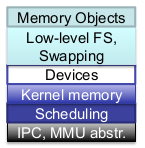
\includegraphics[width=\linewidth]{Assets/AdvancedOperatingSystems-l4-first-g.png} &
        %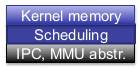
\includegraphics[width=\linewidth]{Assets/AdvancedOperatingSystems-L4-second-g.png} &
        %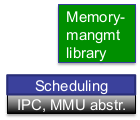
\includegraphics[width=\linewidth]{Assets/AdvancedOperatingSystems-l4-third-g.png}\tabularnewline
        %180 syscalls & \textasciitilde7 syscalls & \textasciitilde3
        %syscalls\tabularnewline
        %100 kLOC & \textasciitilde10 kLOC & 9 kLOC\tabularnewline
        %100 \$\textbackslash mu s\$ IPC & \textasciitilde1 \$\textbackslash mu
        %s\$ IPC & \$0,2-1 \textbackslash mu s\$ IPC\tabularnewline
        %\bottomrule
        %\end{longtable}
    \end{itemize*}


    \paragraph{Mikrokernel-Designprinzipien}

    \begin{itemize*}
        \item
        Was gehört in einen Mikrokern?
        \begin{itemize*}
            \item Liedtke: Unterscheidung zwischen Konzepten und deren Implementierung
            \item bestimmende Anforderungen an beide: \begin{itemize*} \item Konzeptsicht $\rightarrow$ Funktionalität, \item Implementierungssicht $\rightarrow$ Performanz \end{itemize*}
            \item $\rightarrow$ 1. $\mu$Kernel-Generation: Konzept durch Performanzentscheidungen aufgeweicht
            \item $\rightarrow$ Effekt in der Praxis genau gegenteilig: schlechte (IPC-) Performanz!
        \end{itemize*}
    \end{itemize*}

    \begin{quote}
        ,,The determining criterion used is functionality, not performance. More
        precisely, a concept is tolerated inside the $\mu$-kernel only if moving it
        outside the kernel, i.e. permitting competing implementations, would
        prevent the implementation of the systems`s required functionality .''
        {[}Jochen Liedtke{]}
    \end{quote}

    Designprinzipien für Mikrokernel-Konzept:

    \begin{itemize*}
        \item
        $\rightarrow$ Annahmen hinsichtlich der funktionalen
        Anforderungen:
    \end{itemize*}

    \begin{enumerate*}
        \item
        System interaktive und nicht vollständig vertrauenswürdige
        Applikationen unterstützen ( $\rightarrow$ HW-Schutz,
        -Multiplexing),
        \item
        Hardware mit virtueller Speicherverwaltung und Paging
    \end{enumerate*}

    Designprinzipien:

    \begin{enumerate*}
        \item
        Autonomie: ,,Ein Subsystem (Server)muss so implementiert werden
        können, dass es von keinem anderen Subsystem gestört oder korrumpiert
        werden kann.''
        \item
        Integrität: ,,Subsystem (Server) \$S\_1\$ muss sich auf Garantien von
        \$S\_2\$ verlassen können. D.h. beide Subsysteme müssen miteinander
        kommunizieren können, ohne dass ein drittes Subsystem diese
        Kommunikation stören, fälschen oder abhören kann.''
    \end{enumerate*}

    L4: Speicherabstraktion

    \begin{itemize*}
        \item
        Adressraum: Abbildung, die jede virtuelle Seite auf einen physischen
        Seitenrahmen abbildet oder als ,,nicht zugreifbar'' markiert
        \item
        Implementierung über Seitentabellen, unterstützt durch MMU-Hardware
        \item
        Aufgabe des Mikrokernels (als gemeinsame obligatorische Schicht aller
        Subsysteme): muss Hardware-Konzept des Adressraums verbergen und durch
        eigenes Adressraum-Konzept überlagern (sonst Implementierung von
        VMM-Mechanismen durch Server unmöglich)
        \item
        Mikrokernel-Konzept des Adressraums:
        \begin{itemize*}
            \item muss Implementierung von beliebigen virtuellen Speicherverwaltungs-und -schutzkonzepten oberhalb des Mikrokernels (d.h. in den Subsystemen) erlauben
            \item sollte einfach und dem Hardware-Konzept ähnlich sein
        \end{itemize*}
        \item
        Idee: abstrakte Speicherverwaltung
        \begin{itemize*}
            \item rekursive Konstruktion und Verwaltung der Adressräume auf Benutzer-(Server-)Ebene
            \item Mikrokernel stellt dafür genau drei Operationen bereit: \begin{enumerate*} \item grant(x) - Server \$S\$ überträgt Seite \$x\$ seines AR in AR von Empfänger \$S`\$ \item map(x) - Server \$S\$ bildet Seite \$x\$ seines AR in AR von Empfänger \$S`\$ ab \item flush(x) - Server \$S\$ entfernt (flusht) Seite x seines AR aus allen fremden AR \end{enumerate*}
        \end{itemize*}
    \end{itemize*}

    Hierarchische Adressräume

    \begin{itemize*}
        \item
        Rekursive Konstruktion der Adressraumhierarchie
        \begin{itemize*}
            \item Server und Anwendungenkönnen damit ihren Klienten Seiten des eigenen Adressraumes zur Verfügung stellen
            \item Realspeicher: Ur-Adressraum, vom $\mu$Kernel verwaltet
            \item Speicherverwaltung(en), Paging usw.: vollständig außerhalb des $\mu$-Kernels realisiert
            %\item
            % %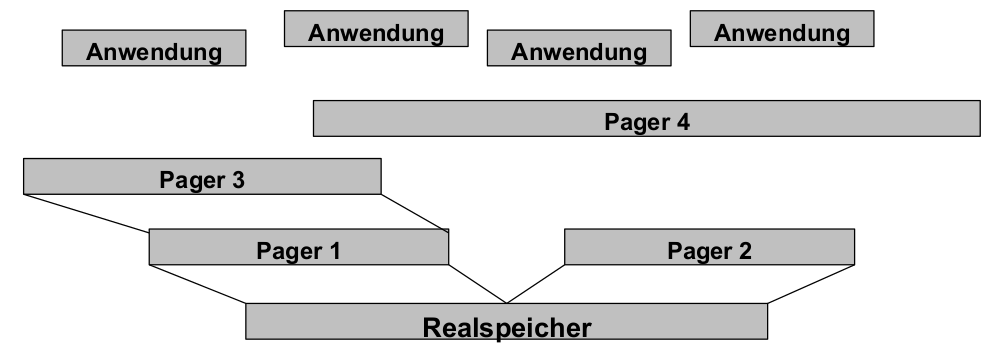
\includegraphics[width=\linewidth]{Assets/AdvancedOperatingSystems-adressraumhierarchie.png}
        \end{itemize*}
    \end{itemize*}

    L4: Threadabstraktion

    \begin{itemize*}
        \item
        Thread
        \begin{itemize*}
            \item innerhalb eines Adressraumesablaufende Aktivität
            \item $\rightarrow$ Adressraumzuordnung ist essenziell für Threadkonzept (Code + Daten) \begin{itemize*} \item Bindung an Adressraum: dynamisch oder fest \item Änderung einer dynamischen Zuordnung: darf nur unter vertrauenswürdiger Kontrolle erfolgen (sonst: fremde Adressräume les- und korrumpierbar) \end{itemize*}
        \end{itemize*}
        \item
        Designentscheidung
        \begin{itemize*}
            \item $\rightarrow$ Autonomieprinzip
            \item $\rightarrow$ Konsequenz: Adressraumisolation
            \item $\rightarrow$ entscheidender Grund zur Realisierung des Thread-Konzepts innerhalb des Mikrokernels
        \end{itemize*}
    \end{itemize*}

    IPC

    \begin{itemize*}
        \item
        Interprozess-Kommunikation
        \begin{itemize*}
            \item Kommunikation über Adressraumgrenzen: vertrauenswürdig kontrollierte Aufhebung der Isolation
            \item $\rightarrow$ essenziell für (sinnvolles) Multitasking und -threading
        \end{itemize*}
        \item
        Designentscheidung
        \begin{itemize*}
            \item $\rightarrow$ Integritätsprinzip
            \item $\rightarrow$ wir haben schon: vertrauenswürdige Adressraumisolation im $\mu$Kernel
            \item $\rightarrow$ grundlegendes IPC-Konzepts innerhalb des Mikrokernels (flexibel und dynamisch durch Server erweiterbar, analog Adressraumhierarchie)
        \end{itemize*}
    \end{itemize*}

    Identifikatoren

    \begin{itemize*}
        \item
        Thread-und Ressourcenbezeichner
        \begin{itemize*}
            \item müssen vertrauenswürdig vergeben (authentisch und i.A. persistent) und verwaltet(eindeutig und korrekt referenzierbar)werden
            \item $\rightarrow$ essenziell für (sinnvolles) Multitasking und -threading
            \item $\rightarrow$ essenziell für vertrauenswürdige Kernel-und Server-Schnittstellen
        \end{itemize*}
        \item
        Designentscheidung
        \begin{itemize*}
            \item $\rightarrow$ Integritätsprinzip
            \item $\rightarrow$ ID-Konzept innerhalb des Mikrokernels (wiederum: durch Server erweiterbar)
        \end{itemize*}
    \end{itemize*}

    Lessons Learned

    \begin{enumerate*}
        \item
        Ein minimaler Mikrokernel
        \begin{itemize*}
            \item soll Minimalmenge an geeigneten Abstraktionenzur Verfügung stellen:
            \item flexibel genug, um Implementierung beliebiger Betriebssysteme zu ermöglichen
            \item Nutzung umfangreicher Mengeverschiedener Hardware-Plattformen
        \end{itemize*}
        \item
        Geeignete, funktional minimale Mechanismen im $\mu$Kern:
        \begin{itemize*}
            \item Adressraum mit map-, flush-, grant-Operation
            \item Threadsinklusive IPC
            \item eindeutige Identifikatoren
        \end{itemize*}
        \item
        Wahl der geeigneten Abstraktionen:
        \begin{itemize*}
            \item kritischfür Verifizierbarkeit ( $\rightarrow$ Robustheit), Adaptivität und optimierte Performanz des Mikrokerns
        \end{itemize*}
        \item
        Bisherigen $\mu$-Kernel-Abstraktionskonzepte:
        \begin{enumerate*}
            \def\labelenumii{\arabic{enumii}.}
            \item ungeeignete
            \item zu viele
            \item zu spezialisierte u. inflexible Abstraktionen
        \end{enumerate*}
        \item
        Konsequenzen für Mikrokernel-Implementierung
        \begin{itemize*}
            \item müssen für jeden Prozessortyp neu implementiert werden
            \item sind deshalb prinzipiell nicht portierbar $\rightarrow$ L3-und L4-Prototypen by J. Liedtke: 99\% Assemblercode
        \end{itemize*}
        \item
        innerhalb eines Mikrokernels sind
        \begin{enumerate*}
            \def\labelenumii{\arabic{enumii}.}
            \item grundlegende Implementierungsentscheidungen
            \item meiste Algorithmen u. Datenstrukturen
        \end{enumerate*}
        \begin{itemize*}
            \item von Prozessorhardware abhängig
        \end{itemize*}
    \end{enumerate*}

    \begin{itemize*}
        \item
        Fazit:
        \begin{itemize*}
            \item Mikrokernelmit akzeptabler Performanz: hardwarespezifische Implementierung minimalerforderlicher, vom Prozessortyp unabhängiger Abstraktionen
            %\item
            % %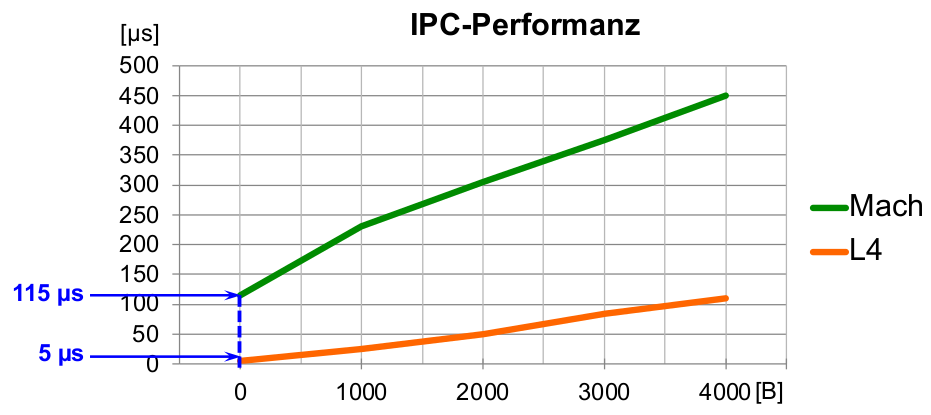
\includegraphics[width=\linewidth]{Assets/AdvancedOperatingSystems-l4-ipc-performance.png}
        \end{itemize*}
    \end{itemize*}

    Heutige Bedeutung

    \begin{itemize*}
        \item
        nach Tod von J. Liedtke (2001) auf Basis von L4 zahlreiche moderne BS
        \item
        L4 heute: Spezifikation eines Mikrokernels (nicht Implementierung)
        \item
        %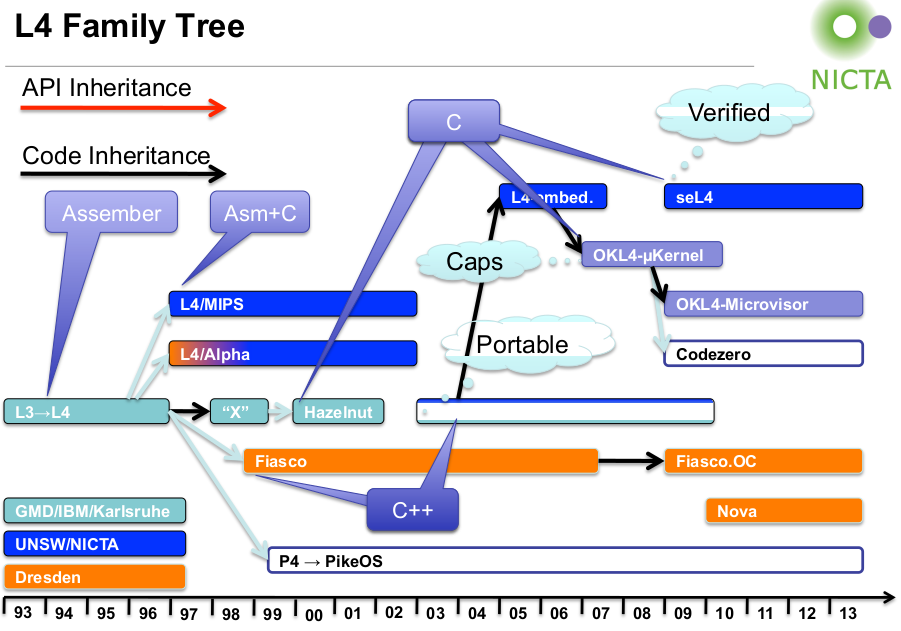
\includegraphics[width=\linewidth]{Assets/AdvancedOperatingSystems-l4-family.png}
        \item
        Einige Weiterentwicklungen:
        \item
        TU Dresden (Hermann Härtig): Neuimplementierung in C++ (L4/Fiasco),
        Basis des Echtzeit-Betriebssystems DROPS, der
        VirtualisierungsplattformNOVA (genauer: Hypervisor) und des adaptiven
        BS-Kernels Fiasco.OC
        \item
        University ofNew South Wales (UNSW), Australien (Gernot Heiser):
        \begin{itemize*}
            \item Implementierung von L4 auf verschiedenen 64 - Bit-Plattformen, bekannt als L4/MIPS, L4/Alpha
            \item Implementierung in C (Wartbarkeit, Performanz)
            \item Mit L4Ka::Pistachio bisher schnellste Implementierung von botschaftenbasierterIPC (2005: 36 Zyklen auf Itanium-Architektur)
            \item seit 2009: seL4, erster formal verifizierter BS-Kernel (d.h. mathematisch bewiesen, dass Implementierung funktional korrekt ist und nachweislich keinen Entwurfsfehler enthält)
        \end{itemize*}
    \end{itemize*}

    Zwischenfazit

    \begin{itemize*}
        \item
        Begrenzung von Fehlerausbreitung ( $\rightarrow$
        Folgen von errors ):
        \item
        konsequent modularisierte Architektur aus Subsystemen
        \item
        Isolationsmechanismen zwischen Subsystemen
        \item
        Konsequenzen für BS-Kernel:
        \item
        statische Isolation auf Quellcodeebene $\rightarrow$
        strukturierte Programmierung
        \item
        dynamische Isolation zur Laufzeit $\rightarrow$
        private virtuelle Adressräume
        \item
        Architektur, welche diese Mechanismen komponiert: Mikrokernel
        \item
        Was haben wir gewonnen?
        \item
        \cmark Adressraumisolation für sämtlichen nichtvertrauenswürdigen Code
        \item
        \cmark keine privilegierten Instruktionen in nvw. Code (Serverprozesse)
        \item
        \cmark geringe Größe (potenziell: Verifizierbarkeit) des Kernels
        \item
        \cmark neben Robustheit: Modularitätund Adaptivitätdes Kernels
        \item
        Und was noch nicht?
        \begin{itemize*}
            \item \xmark Behandlung von Ausfällen ( $\rightarrow$ abstürzende Gerätetreiber ...)
        \end{itemize*}
    \end{itemize*}


    \subsection{3.5 Micro-Reboots}

    \begin{itemize*}
        \item
        Beobachtungen am Ausfallverhalten von BS:
        \item
        Kernelfehler sind (potenziell) fatal für gesamtes System
        \item
        Anwendungsfehler sind es nicht
        \item
        $\rightarrow$ kleiner Kernel = geringeres Risiko von
        Systemausfällen
        \item
        $\rightarrow$ durch BS-Code in Serverprozessen:
        verbleibendes Risiko unabhängiger Teilausfälle von BS-Funktionalität
        (z.B. FS, Treiberprozesse, GUI, ...)
        \item
        Ergänzung zu Isolationsmechanismen:
        \item
        Mechanismen zur Behandlung von Subsystem-Ausfällen
        \item
        = Mechanismen zur Behandlung Anwendungs-, Server- und
        Gerätetreiberfehlen
        \item
        $\rightarrow$ Micro-Reboots
    \end{itemize*}

    Ansatz

    \begin{itemize*}
        \item
        wir haben:
        \item
        kleinen, ergo vertrauenswürdigen (als fehlerfrei angenommenen)$\mu$Kernel
        \item
        BS-Funktionalität in bedingt vertrauenswürdigen Serverprozessen
        (kontrollierbare, aber wesentlich größere Codebasis)
        \item
        Gerätetreiber und Anwendungen in nicht vertrauenswürdigen Prozessen
        (nicht kontrollierbare Codebasis)
        \item
        wir wollen:
        \item
        Systemausfälle verhindern durch Vermeidung von errors im Kernel
        $\rightarrow$ höchste Priorität
        \item
        Treiber-und Serverausfälle minimieren durch Verbergen ihrer
        Auswirkungen $\rightarrow$ nachgeordnete Priorität
        (Best-Effort-Prinzip)
        \item
        Idee:
        \begin{itemize*}
            \item Systemausfälle $\rightarrow$ $\mu$Kernel
            \item Treiber-und Serverausfälle $\rightarrow$ Neustart durch spezialisierten Serverprozess
        \end{itemize*}
    \end{itemize*}

    Beispiel: Ethernet-Treiberausfall

    \begin{itemize*}
        \item
        %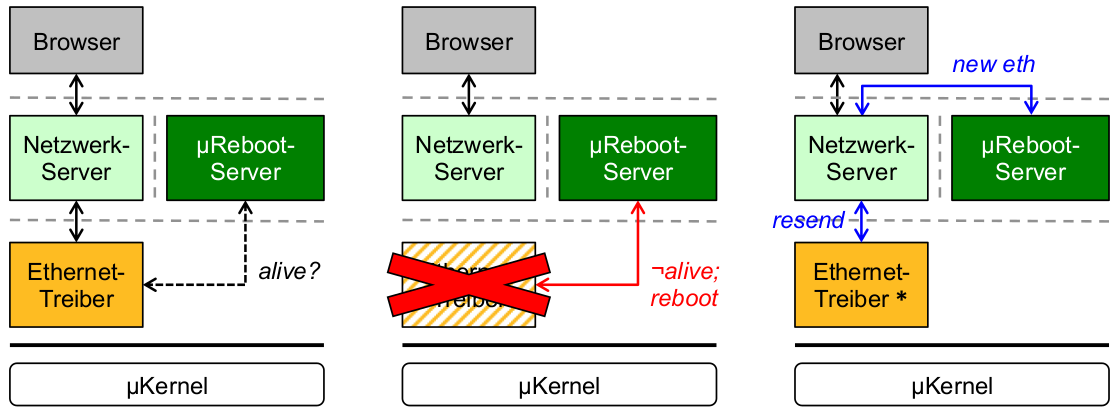
\includegraphics[width=\linewidth]{Assets/AdvancedOperatingSystems-ethernet-treiberausfall.png}
        \item
        schwarz: ausfallfreie Kommunikation
        \item
        rot: Ausfall und Behandlung
        \item
        blau: Wiederherstellung nach Ausfall
    \end{itemize*}

    Beispiel: Dateisystem-Serverausfall

    \begin{itemize*}
        \item
        %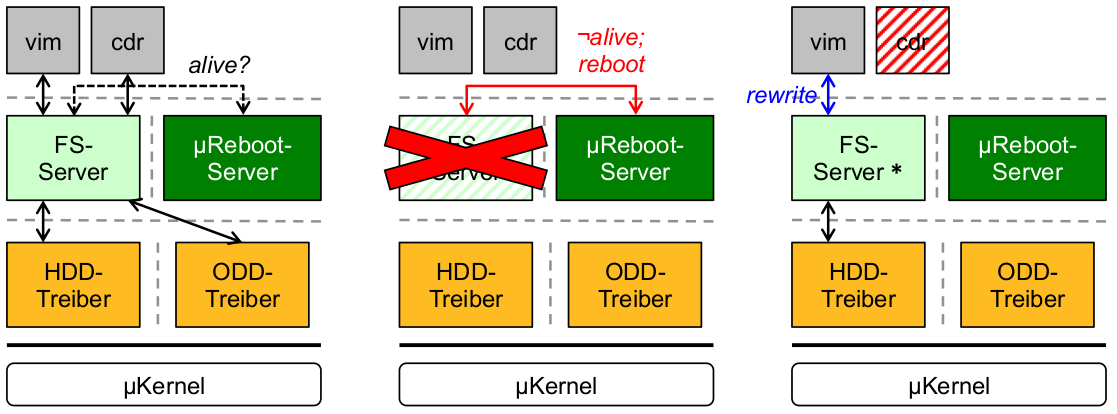
\includegraphics[width=\linewidth]{Assets/AdvancedOperatingSystems-dateisystem-serverausfall.png}
        \item
        schwarz: ausfallfreie Kommunikation
        \item
        rot: Ausfall und Behandlung
        \item
        blau: Wiederherstellung nach Ausfall
    \end{itemize*}


    \subsection{Beispiel-Betriebssystem:
        MINIX}

    \begin{itemize*}
        \item
        Ziele:
        \item
        robustes Betriebssystems
        \item
        $\rightarrow$ Schutz gegen Sichtbarwerden von
        Fehlern(= Ausfälle) für Nutzer
        \item
        Fokus auf Anwendungsdomänen: Endanwender-Einzelplatzrechner (Desktop,
        Laptop, Smart*) und eingebettete Systeme
        \item
        Anliegen: Robustheit \textgreater{} Verständlichkeit \textgreater{}
        geringer HW-Bedarf
        \item
        aktuelle Version: MINIX 3.3.0
    \end{itemize*}

    Architektur

    \begin{itemize*}
        \item
        Kommunikationsschnittstellen ...
        \begin{itemize*}
            %\item
            % %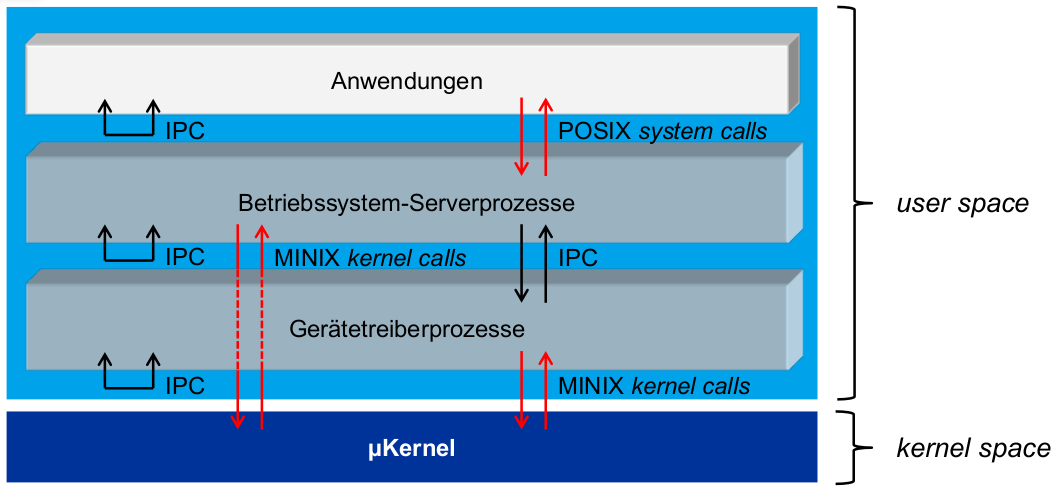
\includegraphics[width=\linewidth]{Assets/AdvancedOperatingSystems-minix-architektur.png}
            \item ... für Anwendungen (weiß): Systemaufrufe im POSIX-Standard
            \item ... für Serverprozesse (grau): \begin{itemize*} \item untereinander: IPC (botschaftenbasiert) \item mit Kernel: spezielle MINIX-API (kernel calls), für Anwendungsprozesse gesperrt \end{itemize*}
        \end{itemize*}
        \item
        Betriebssystem-Serverprozesse:
        \item
        %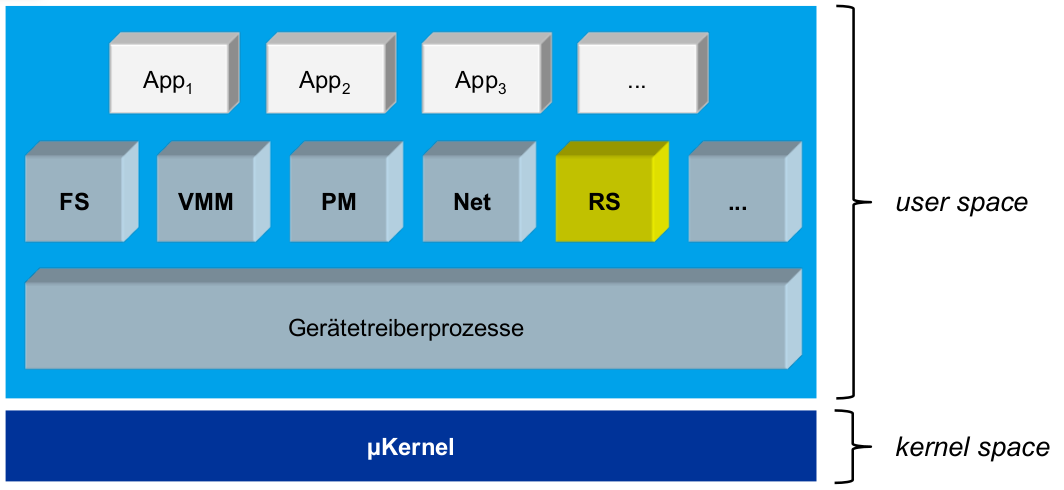
\includegraphics[width=\linewidth]{Assets/AdvancedOperatingSystems-minix-architektur-bs.png}
        \item
        Dateisystem (FS)
        \item
        Prozessmanagement (PM)
        \item
        Netzwerkmanagement (Net)
        \item
        Reincarnation Server (RS) $\rightarrow$ Micro-Reboots
        jeglicher Serverprozesse
        \item
        (u. a.) ...
        \item
        Kernelprozesse:
        \item
        systemtask
        \item
        clocktask
    \end{itemize*}

    Reincarnation Server

    \begin{itemize*}
        \item
        Implementierungstechnik für Micro-Reboots:
        \item
        Prozesse zum Systemstart ( $\rightarrow$ Kernel
        Image): system, clock, init, rs
        \begin{itemize*}
            \item system, clock: Kernelprogramm
            \item init: Bootstrapping (Initialisierung von rs und anderer BS-Serverprozesse), Fork der Login-Shell (und damit sämtlicher Anwendungsprozesse)
            \item rs: Fork sämtlicher BS-Serverprozesse, einschließlich Gerätetreiber
        \end{itemize*}
        \item
        %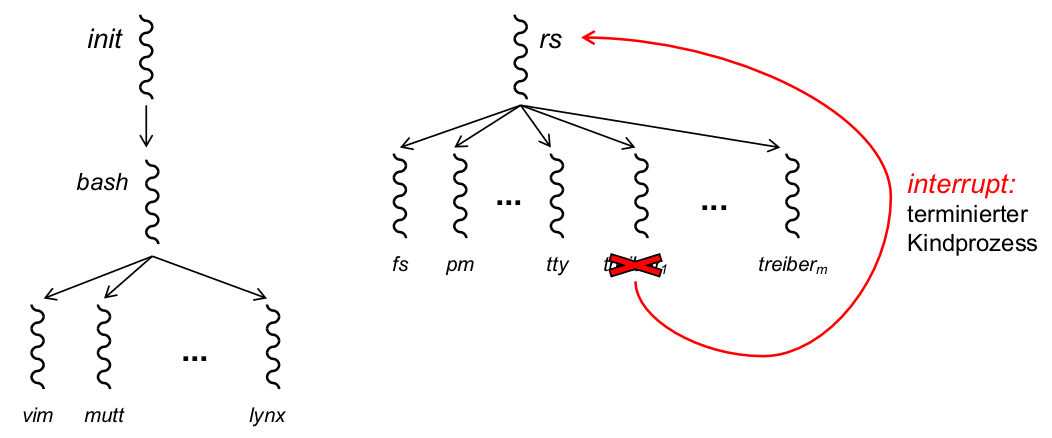
\includegraphics[width=\linewidth]{Assets/AdvancedOperatingSystems-minix-reincarnation-server.png}
    \end{itemize*}

    MINIX: Ausprobieren

    \begin{itemize*}
        \item
        \href{https://wiki.minix3.org/doku.php?id=www:getting-started:start}{ausführliche
            Dokumentation}
        \item
        \href{https://wiki.minix3.org/doku.php?id=www:download:start}{vorkompiliertes
            Kernel-Image zum Installieren (VirtualBox, VMWare, ...)}
    \end{itemize*}


    \subsection{Verfügbarkeit}

    \begin{itemize*}
        \item
        komplementäre NFE zu Robustheit: Verfügbarkeit ( availability )
        \begin{itemize*}
            \item Zur Erinnerung: Untereigenschaften von Verlässlichkeit
        \end{itemize*}
        \begin{enumerate*}

            \item Verfügbarkeit (availability)
            \item Robustheit (robustness, reliability)
        \end{enumerate*}
        \item
        Beziehung:
        \begin{itemize*}
            \item Verbesserung von Robustheit $\rightarrow$ Verbesserung von Verfügbarkeit
            \item Robustheitsmaßnahmen hinreichend , nicht notwendig (hochverfügbare Systeme können sehr wohl von Ausfällen betroffen sein...)
        \end{itemize*}
        \item
        eine weitere komplementäre NFE:
        \begin{itemize*}
            \item Robustheit $\rightarrow$ Sicherheit (security)
        \end{itemize*}
    \end{itemize*}

    Allgemeine Definition: Der Grad, zu welchem ein System oder eine
    Komponente funktionsfähig und zugänglich (erreichbar) ist,wann immer
    seine Nutzung erforderlichist. (IEEE)

    genauer quantifiziert:

    \begin{itemize*}
        \item
        Der Anteil an Laufzeit eines Systems, in dem dieses seine
        spezifizierte Leistung erbringt.
        \item
        %\includegraphics[width=\linewidth]{Assets/AdvancedOperatingSystems-verfügbarkeit-laufzeit.png}
        \item
        Availability= Total Uptime/ Total Lifetime= MTTF / (MTTF + MTTR)
        \begin{itemize*}
            \item MTTR: Mean Time to Recovery ... Erwartungswert für TTR
            \item MTTF: Mean Time to Failure ... Erwartungswert für TTF
        \end{itemize*}
        \item
        einige Verfügbarkeitsklassen: \textbar{} Verfügbarkeit \textbar{}
        Ausfallzeit pro Jahr \textbar{} Ausfallzeit pro Woche \textbar{}
        \textbar{} -\/-\/-\/-\/-\/-\/-\/-\/-\/-\/-\/-\/- \textbar{}
        -\/-\/-\/-\/-\/-\/-\/-\/-\/-\/-\/-\/-\/-\/-\/-\/-\/-\/-\/- \textbar{}
        -\/-\/-\/-\/-\/-\/-\/-\/-\/-\/-\/-\/-\/-\/-\/-\/-\/-\/-\/-\/-
        \textbar{} \textbar{} 90\% \textbar{} \textgreater{} 1 Monat
        \textbar{} ca. 17 Stunden \textbar{} \textbar{} 99\% \textbar{} ca. 4
        Tage \textbar{} ca. 2 Stunden \textbar{} \textbar{} 99,9\% \textbar{}
        ca. 9 Stunden \textbar{} ca. 10 Minuten \textbar{} \textbar{} 99,99\%
        \textbar{} ca. 1 Stunde \textbar{} ca. 1 Minute \textbar{} \textbar{}
        99,999\% \textbar{} ca. 5 Minuten \textbar{} ca. 6 Sekunden \textbar{}
        \textbar{} 99,9999\% \textbar{} ca. 2 Sekunden \textbar{}
        \textless\textless{} 1 Sekunde \textbar{}
        \item
        Hochverfügbarkeitsbereich (gefeierte ,,five nines'' availability)
        \item
        Maßnahmen:
        \item
        Robustheitsmaßnahmen
        \item
        Redundanz
        \item
        Ausfallmanagement
    \end{itemize*}


    \subsubsection{QNX Neutrino: Hochverfügbares
        Echtzeit-BS}

    Überblick QNX:

    \begin{itemize*}
        \item
        Mikrokern-Betriebssystem
        \item
        primäres Einsatzfeld: eingebettete Systeme, z.B. Automobilbau
        \item
        Mikrokernarchitektur mit Adressraumisolation für Gerätetreiber
        \item
        (begrenzt) dynamische Micro-Rebootsmöglich
        \item
        $\rightarrow$ Maximierung der Uptime des Gesamtsystems
    \end{itemize*}

    Hochverfügbarkeitsmechanismen:

    \begin{enumerate*}
        \item
        ,,High-Avalability-Manager'': Laufzeit-Monitor, der Systemdienste oder
        Anwendungsprozesse überwacht und neustartet
        $\rightarrow$ $\mu$Reboot-Server
        \item
        ,,High-Availability-Client-Libraries'': Funktionen zur transparenten
        automatischen Reboot für ausgefallene Server-Verbindungen
    \end{enumerate*}


    \section{Sicherheit}


    \subsection{Motivation}

    Medienberichte zu IT-Sicherheitsvorfällen:

    \begin{itemize*}
        \item
        27.-28.11.2016: Ausfälle von über 900.000 Kundenanschlüssen der
        Deutschen Telekom
        \begin{itemize*}
            \item Bundesamt für Sicherheit in der Informationstechnik (BSI): weltweiter Angriff auf ausgewählte Fernverwaltungsports von DSL-Routern, um angegriffene Geräte mit Schadsoftware zu infizieren
            \item Angreiferziel: Missbrauch der Hardware für eigentliche Angriffe (Botnet)
        \end{itemize*}
        \item
        15.05.-06.06.2019: Ransomware-Angriff zur Erpressung der Heise
        Verlagsgruppe
        \begin{itemize*}
            \item Infektion eines Rechners im lokalen Netz durch Malware in eMail-Anhang (Trojaner)
            \item Täuschung des Nutzers: Schadcode mit Administratorrechten ausgeführt (Spezialfall von Malware: \emph{Root Kit})
            \item Malwareziel: Verschlüsselungvon Nutzerdaten
            \item Angreiferziel: Erspressungvon Lösegeld für Entschlüsselung
        \end{itemize*}
    \end{itemize*}

    Was sichere Betriebssysteme erreichen können ... und was nicht:
    \href{https://www.youtube.com/watch?v=opRMrEfAIiI\&t=}{youtube}


    \subsection{Terminologie}

    Achtung zwei unterschiedliche ,,Sicherheiten''

    \begin{enumerate*}
        \item
        Security (IT-Sicherheit, Informationssicherheit)
        \begin{itemize*}
            \item Ziel: Schutz \textbf{des} Rechnersystems
            \item hier besprochen
            \item Systemsicherheit
        \end{itemize*}
        \item
        Safety (Funktionale Sicherheit, Betriebssicherheit)
        \begin{itemize*}
            \item Ziel: Schutz \textbf{vor} einem Rechnersystem
            \item an dieser Stelle nicht besprochen
        \end{itemize*}
    \end{enumerate*}

    Eine (unvollständige) Taxonomie:

    \begin{itemize*}
        \item
        %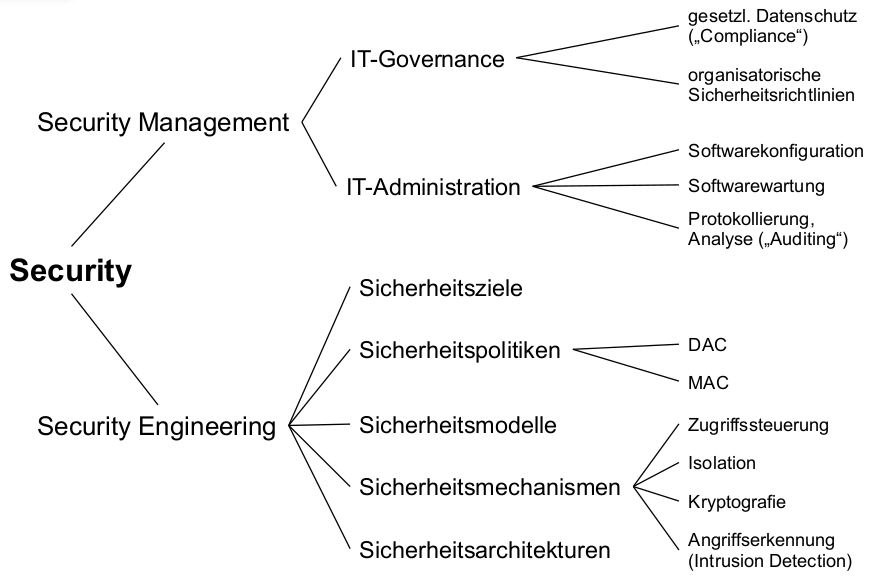
\includegraphics[width=\linewidth]{Assets/AdvancedOperatingSystems-sicherheit-taxonomie.png}
    \end{itemize*}


    \subsection{Sicherheitsziele}

    Allgemeines Ziel von IT-Sicherheit i.S.v. Security ... ein Rechnersystem
    sicher zu machen gegen Schäden durch zielgerichtete Angriffe,
    insbesondere in Bezug auf die Informationen, die in solchen Systemen
    gespeichert, verarbeitet und übertragen werden. (Programme sind somit
    ebenfalls als Informationen zu verstehen.)

    Cave! Insbesondere für Sicherheitsziele gilt: Daten
    \$\textbackslash not=\$ Informationen

    Sicherheitsziele: sukzessive Konkretisierungen dieser Allgemeinformel
    hinsichtlich anwendungsspezifischer Anforderungen


    \subparagraph{Abstrakte Ziele:}

    \begin{enumerate*}
        \item
        Vertraulichkeit (Confidentiality)
        \item
        Integrität (Integrity)
        \item
        Verfügbarkeit (Availability)
        \item
        Authentizität (Authenticity)
        \item
        Verbindlichkeit = Nichtabstreitbarkeit (Non-repudiability)
    \end{enumerate*}

    Abstrakte Ziele dienen zur Ableitung konkreter Sicherheitsziele. Wir
    definieren sie als Eigenschaften von gespeicherten oder übertragenen
    Informationen ...

    \begin{itemize*}
        \item
        Vertraulichkeit: ... nur für einen autorisierten Nutzerkreis
        zugänglich (i.S.v. interpretierbar) zu sein.
        \item
        Integrität: ... vor nicht autorisierter Veränderung geschützt zu sein.
        \item
        Verfügbarkeit: ... autorisierten Nutzern in angemessener Frist
        zugänglich zu sein.
        \item
        Authentizität: ... ihren Urheber eindeutig erkennen zu können.
        \item
        Verbindlichkeit: ... sowohl integer als auch authentisch zu sein.
    \end{itemize*}


    \subparagraph{Schadenspotenzial}

    \begin{enumerate*}
        \item
        Vandalismus, Terrorismus
    \end{enumerate*}

    \begin{itemize*}
        \item
        reine Zerstörungswut
    \end{itemize*}

    \begin{enumerate*}
        \setcounter{enumi}{1}
        \item
        Systemmissbrauch
    \end{enumerate*}

    \begin{itemize*}
        \item
        illegitime Ressourcennutzung, Ziel i.d.R.: hocheffektive Folgeangriffe
        \item
        Manipulationvon Inhalten ( $\rightarrow$
        Desinformation)
    \end{itemize*}

    \begin{enumerate*}
        \setcounter{enumi}{2}
        \item
              (Wirtschafts-) Spionage und Diebstahl
    \end{enumerate*}

    \begin{itemize*}
        \item
        Verlust der Kontrolle über kritisches Wissen
        ( $\rightarrow$ Risikotechnologien)
        \item
        immense wirtschaftliche Schäden ( $\rightarrow$
        Technologieführer, Patentinhaber)
        \item
        z.B. Diebstahl von industriellem Know-How
    \end{itemize*}

    \begin{enumerate*}
        \setcounter{enumi}{3}
        \item
        Betrug, persönliche Bereicherung
    \end{enumerate*}

    \begin{itemize*}
        \item
        wirtschaftliche Schäden
    \end{itemize*}

    \begin{enumerate*}
        \setcounter{enumi}{4}
        \item
        Sabotage, Erpressung
    \end{enumerate*}

    \begin{itemize*}
        \item
        Außerkraftsetzen lebenswichtiger Infrastruktur (z.B. schon
        Registrierkassen)
        \item
        Erpressung von ausgewählten (oder schlicht großen ) Zielgruppen durch
        vollendete, reversible Sabotage ( $\rightarrow$
        Verschlüsselung von Endanwenderinformationen)
    \end{itemize*}


    \subparagraph{Bedrohungen}

    \begin{enumerate*}
        \item
        Eindringlinge (intruders)
        \begin{itemize*}
            \item im engeren Sinne menschliche Angreifer ( ,,Hacker'' ), deren Angriff eine technische Schwachstelleausnutzt ( exploit )
        \end{itemize*}
        \item
        Schadsoftware (malicious software, malware)
        \begin{itemize*}
            \item durch Ausnutzung einer (auch menschlichen) Schwachstelle zur Ausführung gebrachte Programme, die (teil-) automatisierte Angriffe durchführen
            \item Trojanische Pferde (trojan horses): scheinbar nützliche Software, die verborgene Angriffsfunktionalität enthält
            \item Viren, Würmer (viruses, worms): Schadsoftware, die Funktionalität zur eigenen Vervielfältigung und/oder Modifikation beinhaltet
            \item Logische Bomben (logicbombs): Code-Sequenz in trojanischen Pferden, deren Aktivierung an System-oder Datumsereignisse gebunden ist
            \item Root Kits
        \end{itemize*}
        \item
        Bots und Botnets
        \begin{itemize*}
            \item (weit-) verteilt ausgeführte Schadsoftware
            \item eigentliches Ziel i.d.R. nicht das jeweils infizierte System
        \end{itemize*}
    \end{enumerate*}


    \subparagraph{Professionelle Malware: Root
        Kit}

    \begin{itemize*}
        \item
        Programm-Paket, das unbemerkt Betriebssystem (und ausgewählte
        Anwendungen) modifiziert, um Administratorrechte zu erlangen
        \begin{itemize*}
            \item Administrator-bzw. Rootrechte: ermöglichen Zugriff auf alle Funktionen und Dienste eines Betriebssystems
            \item Angreifer erlangt vollständige Kontrolle des Systems und kann \begin{itemize*} \item Dateien (Programme) hinzufügen bzw. ändern \item Prozesse überwachen \item über die Netzverbindungen senden und empfangen \item bei all dem Hintertüren für Durchführung und Verschleierung zukünftiger Angriffe platziere \end{itemize*}
            \item Ziele eines Rootkits: \begin{itemize*} \item seine Existenz verbergen \item zu verbergen, welche Veränderungen vorgenommen wurden \item vollständige und irreversible Kontrolle über BS zu erlangen \end{itemize*}
        \end{itemize*}
        \item
        Ein erfolgreicher Root-Kit-Angriff ...
        \begin{itemize*}
            \item ... kann jederzeit
            \item ... mit hochaktuellem und systemspezifischem Wissen über Schwachstellen
            \item ... vollautomatisiert, also reaktiv unverhinderbar
            \item ... unentdeckbar
            \item ... nicht reversibel
            \item ... die uneingeschränkte Kontrolle über das Zielsystem erlangen.
        \end{itemize*}
        \item
        Voraussetzung: eine einzige Schwachstelle...
    \end{itemize*}


    \subparagraph{Schwachstellen}

    \begin{enumerate*}
        \item
        Passwort (begehrt: Administrator-Passwörter...)
    \end{enumerate*}

    \begin{itemize*}
        \item
        ,,erraten''
        \item
        zu einfach, zu kurz, usw.
        \item
        Brute-Force-Angriffe mit Rechnerunterstützung
        \item
        Abfangen ( eavesdropping )
        \item
        unverschlüsselte Übertragung (verteilte Systeme) oder Speicherung
    \end{itemize*}

    \begin{enumerate*}
        \setcounter{enumi}{1}
        \item
        Programmierfehler (Speicherfehler...!)
    \end{enumerate*}

    \begin{itemize*}
        \item
        im Anwenderprogrammen
        \item
        in Gerätemanagern
        \item
        im Betriebssystem
    \end{itemize*}

    \begin{enumerate*}
        \setcounter{enumi}{2}
        \item
        Mangelhafte Robustheit
    \end{enumerate*}

    \begin{itemize*}
        \item
        keine Korrektur fehlerhafter Eingaben
        \item
        buffer overrun/underrun (,, Heartbleed'' )
    \end{itemize*}

    \begin{enumerate*}
        \setcounter{enumi}{3}
        \item
        Nichttechnische Schwachstellen
    \end{enumerate*}

    \begin{itemize*}
        \item
        physisch, organisatorisch, infrastrukturell
        \item
        menschlich ( $\rightarrow$ Erpressung,
        socialengineering )
    \end{itemize*}


    \subparagraph{Zwischenfazit}

    \begin{itemize*}
        \item
        Schwachstellen sind unvermeidbar
        \item
        Bedrohungen sind unkontrollierbar
        \begin{itemize*}
            \item ... und nehmen tendeziellzu!
        \end{itemize*}
    \end{itemize*}

    Beides führt zu operationellen Risiken beim Betrieb eines IT-Systems

    $\rightarrow$ Aufgabe der Betriebssystemsicherheit:
    Auswirkungen operationeller Risiken reduzieren (wo diese nicht vermieden
    werden können...)

    Wie dies geht: Security Engineering


    \subsection{Sicherheitspolitiken}

    \begin{itemize*}
        \item
        Herausforderung: korrekte Durchsetzung von Sicherheitspolitiken
        \item
        Vorgehensweise: Security Engineering
    \end{itemize*}

    \textbar{} \textbar{} \textbar{}
    -\/-\/-\/-\/-\/-\/-\/-\/-\/-\/-\/-\/-\/-\/-\/-\/-\/-\/-\/-\/-\/-
    \textbar{}
    -\/-\/-\/-\/-\/-\/-\/-\/-\/-\/-\/-\/-\/-\/-\/-\/-\/-\/-\/-\/-\/-\/-\/-\/-\/-\/-\/-\/-\/-\/-\/-\/-\/-\/-\/-\/-\/-\/-\/-\/-\/-\/-\/-\/-\/-\/-\/-\/-\/-\/-\/-\/-\/-\/-\/-\/-\/-\/-\/-\/-\/-\/-\/-\/-\/-\/-\/-\/-\/-\/-\/-\/-\/-\/-\/-\/-\/-\/-\/-\/-\/-\/-\/-\/-\/-\/-\/-\/-
    \textbar{} \textbar{} Sicherheitsziele \textbar{} Welche
    Sicherheitsanforderungen muss das Betriebssystem erfüllen? \textbar{}
    \textbar{} Sicherheitspolitik \textbar{} Durch welche Strategien soll es
    diese erfüllen? ( $\rightarrow$ Regelwerk) \textbar{}
    \textbar{} Sicherheitsmechanismen \textbar{} Wie implementiert das
    Betriebssystem seine Sicherheitspolitik? \textbar{} \textbar{}
    Sicherheitsarchitektur \textbar{} Wo implementiert das Betriebssystem
    seine Sicherheitsmechanismen (und deren Interaktion)? \textbar{}


    \subparagraph{Sicherheitspolitiken und
        -modelle}

    Kritischfür korrekten Entwurf, Spezifikation, Implementierung der
    Betriebssystem-Sicherheitseigenschaften!

    Begriffsdefinitionen:

    \begin{itemize*}
        \item
        Sicherheitspolitik (Security Policy): Eine Menge von Regeln, die zum
        Erreichen eines Sicherheitsziels dienen.
        \item
        Sicherheitsmodell (Security Model): Die formale Darstellung einer
        Sicherheitspolitik zum Zweck
        \begin{itemize*}
            \item der Verifikation ihrer Korrektheit
            \item der Spezifikation ihrer Implementierung.
        \end{itemize*}
    \end{itemize*}


    \subparagraph{Zugriffssteuerungspolitiken}

    ... geben Regeln vor, welche durch Zugriffssteuerungsmechanismen in BS
    durchgesetzt werden müssen.

    Zugriffssteuerung (access control): Steuerung, welcher Nutzer oder
    Prozess mittels welcher Operationen auf welche BS-Ressourcen zugreifen
    darf (z.B.: Anwender darf Textdateien anlegen, Administrator darf
    Dateisysteme montieren und System-Logdateien löschen, systemd - Prozess
    darf Prozessdeskriptoren manipulieren, ...)

    Zugriffssteuerungspolitik: konkrete Regeln, welche die Zugriffssteuerung
    in einem BS beschreiben

    Zugriffssteuerungsmodell: Sicherheitsmodell einer
    Zugriffssteuerungspolitik

    Zugriffssteuerungsmechanismus: Implementierung einer
    Zugriffssteuerungspolitik


    \subparagraph{Beispiele für
        BS-Zugriffssteuerungspolitiken}

    klassifiziert nach Semantik der Politikregeln:

    \begin{itemize*}
        \item
        IBAC (Identity-basedAccess Control): Politik spezifiziert, welcher
        Nutzer an welchen Ressourcen bestimmte Rechte hat.
        \begin{itemize*}
            \item Bsp.: ,,Nutzer Anna darf Brief.docx lesen, aber nicht schreiben.''
        \end{itemize*}
        \item
        TE (Type-Enforcement): Politik spezifiziert Rechte durch zusätzliche
        Abstraktion (Typen): welcher Nutzertyp an welchem Ressourcentyp
        bestimmte Rechte hat.
        \begin{itemize*}
            \item Bsp.: ,,Nutzer vom Typ Administrator dürfen Dateien vom Typ Log lesen und schreiben.''
        \end{itemize*}
        \item
        MLS (Multi-Level Security): Politik spezifiziert Rechte, indem aus
        Nutzern und Ressourcen hierarchische Klassen (Ebenen, ,,Levels'')
        gleicher Kritikalität im Hinblick auf Sicherheitsziele gebildet
        werden.
        \begin{itemize*}
            \item Bsp.: ,,Nutzer der Klasse nicht vertrauenswürdig dürfen Dateien der Klasse vertraulich nicht lesen.''
        \end{itemize*}
        \item
        DAC (Discretionary Access Control, auch: wahlfreie Zugriffssteuerung
        ): Aktionen der Nutzer setzen die Sicherheitspolitik (oder wesentliche
        Teile davon) durch. Typisch: Begriff des Eigentümers von
        BS-Ressourcen.
        \begin{itemize*}
            \item Bsp.: ,,Der Eigentümer einer Datei bestimmt (bzw. ändert), welcher Nutzer welche Rechte daran hat.''
        \end{itemize*}
        \item
        MAC (MandatoryAccess Control, auch: obligatorische Zugriffssteuerung
        ): Keine Beteiligung der Nutzer an der Durchsetzungeiner (zentral
        administrierten) Sicherheitspolitik.
        \begin{itemize*}
            \item Bsp.: ,,Anhand ihres Dateisystempfads bestimmt das Betriebssystem, welcher Nutzer welche Rechte an einer Datei hat.''
        \end{itemize*}
    \end{itemize*}


    \subparagraph{Einige Beispiele ...}

    %\begin{longtable}[]{@{}lll@{}}
    %\toprule
    %& DAC & MAC\tabularnewline
    %\midrule
    %\endhead
    %IBAC & Unixoide,Linux, Windows & Linux AppArmor, Mac OS
    %Seatbelt\tabularnewline
    %TE & - & SELinuxEnterprise Linux (RHEL), RedHat\tabularnewline
    %MLS & Windows UAC & SELinux, TrustedBSD\tabularnewline
    %\bottomrule
    %\end{longtable}

    ... und ein Verdacht Eindruck der Effektivität von DAC: ,,{[}...{]} so
    the theory goes. By extension, yes, there may be less malware, but that
    will depend on whether users keep UAC enabled, which depends on whether
    developers write software that works with it and that users stop viewing
    prompts as fast-clicking exercises and actually consider whether an
    elevation request is legitimate.'' (Jesper M. Johansson, TechNet
    Magazine)
    {[}https://technet.microsoft.com/en-us/library/2007.09.securitywatch.aspx,
    Stand: 10.11.2017{]}


    \subsubsection{Traditionell: DAC, IBAC}

    Auszug aus der Unix-Sicherheitspolitik:

    \begin{itemize*}
        \item
        es gibt Subjekte (Nutzer, Prozesse) und Objekte (Dateien, Sockets ...)
        \item
        jedes Objekt hat einen Eigentümer
        \item
        Eigentümer legen Zugriffsrechte an Objekten fest
        ( $\rightarrow$ DAC)
        \item
        es gibt drei Zugriffsrechte: read, write, execute
        \item
        je Objekt gibt es drei Klassen von Subjekten, für die individuell
        Zugriffsrechte vergeben werden können: Eigentümer (,,u''), Gruppe
        (,,g''), Rest der Welt (,,o'')
    \end{itemize*}

    In der Praxis:

    \begin{itemize*}
        \item
        identitätsbasierte (IBAC), wahlfreie Zugriffssteuerung (DAC)
        \item
        hohe individuelle Freiheit der Nutzer bei Durchsetzung der Politik
        \item
        hohe Verantwortung ( ,,Welche Nutzer werden jemals in Gruppe vsbs
        sein...?'' )
    \end{itemize*}

    %\begin{Shaded}
    %\begin{Highlighting}[]
    %\ExtensionTok{{-}rw{-}}\NormalTok{ rw{-} r{-}{-} 1 amthor vsbs 397032 2017{-}11{-}19 12:12 paper.pdf}
    %\end{Highlighting}
    %\end{Shaded}


    \subparagraph{Modellierung:
        Zugriffsmatrix}

    %\begin{longtable}[]{@{}lllll@{}}
    %\toprule
    %acm & paper.pdf & aos-05.pptx & gutachten.tex &
    %worse-engine\tabularnewline
    %\midrule
    %\endhead
    %kühnhauser & rw & - & rw & rx\tabularnewline
    %schlegel & rw & - & - & rx\tabularnewline
    %amthor & rw & rw & - & rx\tabularnewline
    %krause & r & - & - & -\tabularnewline
    %\bottomrule
    %\end{longtable}

    \begin{itemize*}
        \item
        acm (access control matrix): Momentaufnahme der globalen
        Rechteverteilung zu einem definierten ,,Zeitpunkt t''
        \item
        Korrektheitskriterium: Wie kann sich dies nach t möglicherweise
        ändern...? (HRU-Sicherheitsmodell){[}HaRU76{]}
    \end{itemize*}


    \subparagraph{Modellkorrektheit:
        Rechteausbreitung}

    \begin{itemize*}
        \item
        Änderungsbeispiel: kühnhauser nimmt krause in Gruppe vsbs auf ...
        \item
        Rechteausbreitung ( privilegeescalation ), hier verursacht durch eine
        legale Nutzeraktion ( $\rightarrow$ DAC)
        \begin{itemize*}
            \item (Sicherheitseigenschaft: HRU Safety , $\rightarrow$ ,,Systemsicherheit'')
        \end{itemize*}
    \end{itemize*}


    \subsubsection{Modern: MAC, MLS}

    Sicherheitspolitik der Windows UAC ( user account control):

    \begin{itemize*}
        \item
        es gibt Subjekte (Prozesse) und Objekte (Dateisystemknoten)
        \item
        jedem Subjekt ist eine Integritätsklasse zugewiesen:
        \begin{itemize*}
            \item Low: nicht vertrauenswürdig (z.B. Prozesse aus ausführbaren Downloads)
            \item Medium: reguläre Nutzerprozesse, die ausschließlich Nutzerdaten manipulieren
            \item High: Administratorprozesse, die Systemdaten manipulieren können
            \item System: (Hintergrund-) Prozesse, die ausschließlich Betriebssystemdienste auf Anwenderebene implementieren (etwa der Login-Manager)
        \end{itemize*}
        \item
        jedem Objekt ist analog eine dieser Integritätsklassen zugewiesen
        (Kritikalität von z.B. Nutzerdaten vs. Systemdaten)
        \item
        sämtliche DAC-Zugriffsrechte (die gibt es auch) müssen mit einer
        Hierarchie der Integritätsklassen konsistent sein
        ( $\rightarrow$ ein bisschen MAC)
        \item
        Nutzer können diese Konsistenzanforderung selektiv außer Kraft setzen
        ( $\rightarrow$ DAC)
    \end{itemize*}


    \subparagraph{MAC-Modellierung:
        Klassenhierarchie}

    Beispiel: Modelliert durch Relation \$\textbackslash leq\$: gleich oder
    kritischer als

    \$\textbackslash leq=\{( High , Medium ), ( High , Low ), ( Medium , Low
    ), ( High , High ), ( Medium , Medium ), ( Low , Low )\}\$

    \begin{itemize*}
        \item
        repräsentiert Kritikalität hinsichtlich des Sicherheitsziels
        Integrität (Biba-Sicherheitsmodell) {[}Biba77{]}
        \item
        wird genutzt, um legale Informationsflüsse zwischen Subjekten und
        Objekten zu modellieren $\rightarrow$ Schutz vor
        illegalem Überschreiben
        \item
        leitet Zugriffsrechte aus Informationsflüssen ab:
        \begin{itemize*}
            \item Prozess Datei: schreiben
            \item Prozess Datei: lesen
        \end{itemize*}
    \end{itemize*}


    \subparagraph{DAC-Modellierung:
        Zugriffsmatrix}

    %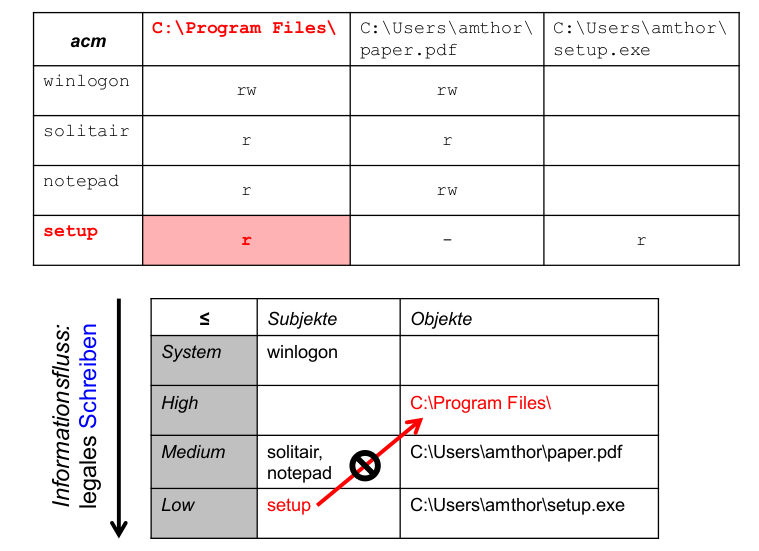
\includegraphics[width=\linewidth]{Assets/AdvancedOperatingSystems-dac-zugriffsmatrix.png}


    \subparagraph{Modellkorrektheit:
        Konsistenz}

    \begin{itemize*}
        \item
        Korrektheitskriterium: Garantiert die Politik, dass acm mit
        \$\textbackslash leq\$ jederzeit konsistent ist? ( BLP Security )
        {[}BeLa76{]}
        \item
        elevation-Mechanismus: verändert nach Nutzeranfrage
        ( $\rightarrow$ DAC) sowohl acm als auch
        \$\textbackslash leq\textbackslash rightarrow\$ konsistenzerhaltend?
        \item
        andere BS-Operationen: verändern unmittelbar nur acm (z.B. mittels
        Dateisystemmanagement) $\rightarrow$
        konsistenzerhaltend?
    \end{itemize*}


    \subsection{Autorisierungsmechanismen}

    Begriffsdefinitionen:

    \begin{itemize*}
        \item
        Sicherheitsmechanismen: Datenstrukturen und Algorithmen, welche die
        Sicherheitseigenschaften eines Betriebssystems implementieren.
        \begin{itemize*}
            \item $\rightarrow$ Sicherheitsmechanismen benötigt man zur Herstellung jeglicher Sicherheitseigenschaften (auch jener, die in unseren Modellen implizit angenommen werden!)
            \item Nutzerauthentisierung ( login - Dientsprogramm, Passwort-Hashing, ...)
            \item Autorisierungsinformationen (Metainformationen über Rechte, MLS-Klassen, TE-Typen, ...)
            \item Autorisierungsmechanismen (Rechteprüfung, Politikadministration, ...)
            \item kryptografische Mechanismen (Verschlüsselungsalgorithmen, Hashfunktionen, ...)
        \end{itemize*}
        \item
        Auswahl im Folgenden: Autorisierungsmechanismen und -informationen
    \end{itemize*}


    \subsubsection{Traditionell: ACLs, SUID}

    Autorisierungsinformationen:

    \begin{itemize*}
        \item
        müssen Subjekte (Nutzer) bzw. Objekte (Dateien, Sockets ...) mit
        Rechten assoziieren $\rightarrow$ Implementierung der
        Zugriffsmatrix ( acm ), diese ist:
        \begin{itemize*}
            \item groß ( $\rightarrow$ Dateianzahl auf Fileserver)
            \item dünn besetzt
            \item in Größe und Inhalt dynamisch veränderlich
            \item $\rightarrow$ effiziente Datenstruktur?
        \end{itemize*}
        \item
        Lösung: verteilte Implementierung der acm als Spaltenvektoren, deren
        Inhalt in den Objekt-Metadaten repräsentiert wird:
        Zugriffssteuerungslisten ( Access Control Lists , ACLs)
    \end{itemize*}


    \subparagraph{ACLs:
        Linux-Implementierung}

    \begin{itemize*}
        \item
        objektspezifischer Spaltenvektor = Zugriffssteuerungsliste
        \item
        Dateisystem-Metainformationen: implementiert in I-Nodes
    \end{itemize*}

    %\begin{Shaded}
    %\begin{Highlighting}[]
    %\ExtensionTok{{-}rw{-}}\NormalTok{ rw{-} r{-}{-} 1 amthor vsbs 397032 2017{-}11{-}19 12:12 paper.pdf}
    %\end{Highlighting}
    %\end{Shaded}


    \paragraph{ACLs:
        Linux-Implementierung}

    Modell einer Unix acm ... \textbar{} \textbar{} lesen \textbar{}
    schreiben \textbar{} ausführen \textbar{} \textbar{}
    -\/-\/-\/-\/-\/-\/-\/-\/-\/-\/-\/-\/-\/-\/-\/-\/-\/-\/-\/-\/- \textbar{}
    -\/-\/-\/-\/- \textbar{} -\/-\/-\/-\/-\/-\/-\/-\/- \textbar{}
    -\/-\/-\/-\/-\/-\/-\/-\/- \textbar{} \textbar{} Eigentümer (,,u'')
    \textbar{} ja \textbar{} ja \textbar{} ja \textbar{} \textbar{} Rest der
    Welt (,,o'') \textbar{} ja \textbar{} nein \textbar{} ja \textbar{}
    \textbar{} Gruppe (,,g'') \textbar{} ja \textbar{} nein \textbar{} ja
    \textbar{}

    \begin{itemize*}
        \item
        3 - elementige Liste
        \item
        3 - elementige Rechtemenge
        \item
        $\rightarrow$ 9 Bits
        \item
        dessen Implementierung kodiert in 16-Bit-Wort: 1 1 1 1 0 1 1 0 1
        \item
        ... und dessen Visualisierung in Linux:
    \end{itemize*}

    %\begin{Shaded}
    %\begin{Highlighting}[]
    %\NormalTok{$ }\FunctionTok{ls}\NormalTok{ {-}alF}
    %\ExtensionTok{drwxr{-}xr{-}x}\NormalTok{ 2 amthor amthor 4096 2017{-}11{-}16 12:01 ./}
    %\ExtensionTok{drwxr{-}xr{-}x}\NormalTok{ 31 amthor amthor 4096 2017{-}11{-}07 12:42 ../}
    %\ExtensionTok{{-}rw{-}rw{-}r{-}{-}}\NormalTok{ 1 amthor vsbs 397032 2017{-}11{-}19 12:12 paper.pdf}
    %\ExtensionTok{{-}rw{-}{-}{-}{-}{-}{-}{-}}\NormalTok{ 1 amthor amthor 120064 2017{-}02{-}07 07:56 draft.tex}
    %\end{Highlighting}
    %\end{Shaded}


    \subparagraph{Autorisierungsmechanismen:
        ACL-Auswertung}

    Subjekte = Nutzermenge eines Linux-Systems... besteht aus Anzahl
    registrierter Nutzer

    \begin{itemize*}
        \item
        jeder hat eindeutige UID (userID), z.B. integer- Zahl
        \item
        Dateien, Prozesse und andere Ressourcenwerden mit UID des
        Eigentümersversehen
        \begin{itemize*}
            \item bei Dateien: Teil des I-Nodes
            \item bei Prozessen: Teil des PCB (vgl. Grundlagen ,,Betriebssysteme'')
            \item standardmäßiger Eigentümer: derjenige, eine Ressource erzeugt hat
        \end{itemize*}
    \end{itemize*}

    Nutzergruppen (groups)

    \begin{itemize*}
        \item
        jeder Nutzer wird durch Eintrag in einer Systemdatei ( /etc/group )
        einer oder mehreren Gruppen zugeordnet( $\rightarrow$
        ACL: ,, g '' Rechte)
    \end{itemize*}

    Superuser oder root... hat grundsätzlich uneingeschränkte Rechte.

    \begin{itemize*}
        \item
        UID = 0
        \item
        darf insbesondere alle Dateien im System lesen, schreiben, ausführen;
        unabhängig von ACL
    \end{itemize*}


    \subparagraph{ACL-Implementierung}

    \begin{itemize*}
        \item
        ACLs:
        \begin{itemize*}
            \item in welchen Kerneloperationen?
            \item welche Kernelschnittstellen (Rechte prüfen, ändern)?
            \item welche Datenstrukturen, wo gespeichert?
        \end{itemize*}
        \item
        acm und ACLs:
        \begin{itemize*}
            \item Vorteile der Listenimplementierung?
            \item Nachteile ggü. zentral implementierter Matrix? (DAC vs. MAC, Administration, Analyse ...)
        \end{itemize*}
        \item
        $\rightarrow$ Übung 2
    \end{itemize*}


    \subparagraph{Nutzerrechte $\rightarrow$
        Prozessrechte}

    bisher: Linux-Sicherheitspolitik formuliert Nutzerrechte an Dateien
    (verteilt gespeichert in ACLs)

    Durchsetzung: basiert auf Prozessrechten

    \begin{itemize*}
        \item
        Annahme: Prozesse laufen mit UID des Nutzers, welcher sie gestartet
        hat und repräsentieren Nutzerintention und Nutzerberechtigungen i.S.d.
        Sicherheitspolitik
        \item
        technisch bedeutet dies: ein Nutzer beauftragt einen anderen Prozess,
        sich zu dublizieren( fork() ) und das gewünschte Programm auszuführen
        ( exec*() )
        \item
        Vererbungsprinzip:
        %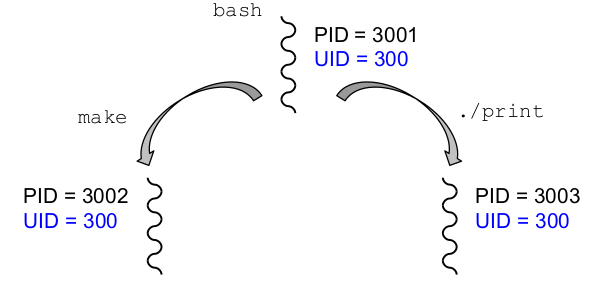
\includegraphics[width=\linewidth]{Assets/AdvancedOperatingSystems-acl-vererbungsprinzip.png}
    \end{itemize*}


    \subparagraph{Autorisierungsmechanismen:
        Set-UID}

    konsequente Rechtevererbung:

    \begin{itemize*}
        \item
        Nutzer können im Rahmen der DAC-Politik ACLs manipulieren
        \item
        Nutzer können (i.A.) jedoch keine Prozess-UIDs manipulieren
        \item
        $\rightarrow$ und genau so sollte es gem.
        Unix-Sicherheitspolitik auch sein!
    \end{itemize*}

    Hintergrund:

    \begin{itemize*}
        \item
        Unix-Philosophie ,, everythingisa file '': BS-Ressourcen wie Sockets,
        IPC-Instanzen, E/A-Gerätehandler als Datei repräsentiert
        $\rightarrow$ identische Schutzmechanismen zum
        regulären Dateisystem
        \item
        somit: Autorisierungsmechanismen zur Begrenzung des Zugriffs auf
        solche Geräte nutzbar (Bsp.: Zugriffe verschiedener Prozesse auf einem
        Drucker müssen koordiniert, ggf. eingeschränkt werden)
        \item
        dazu muss
        \begin{itemize*}
            \item \emph{root} bzw. zweckgebundener Nutzer Eigentümer des Druckers sein
            \item ACL als \texttt{rw-\ -\/-\/-\ -\/-\/-} gesetzt sein
        \end{itemize*}
    \end{itemize*}

    Folge:

    \begin{itemize*}
        \item
        Nutzerprozesse könnten z.B. nicht drucken ...
    \end{itemize*}

    Lösung: Mechanismus zur Rechtedelegation

    \begin{itemize*}
        \item
        implementiert durch ein weiteres ,,Recht'' in ACL: SUID-Bit (,,
        setUID'' )
        \item
        Programmausführung modifiziert Kindprozess, so dass UID des
        Programmeigentümers (im Bsp.: root ) seine Rechte bestimmt
        \item
        Technik: eine von UID abweichende Prozess-Metainformation
        ( $\rightarrow$ PCB) effektive UID (eUID) wird
        tatsächlich zur Autorisierung genutzt
        \item
        \texttt{-rws\ rws\ r-x\ 1\ root\ root\ 2\ 2011-10-01\ 16:00\ print}
    \end{itemize*}

    Strategie für sicherheitskritische Linux-Programme

    \begin{itemize*}
        \item
        Eigentümer: root
        \item
        SUID-Bit: gesetzt
        \item
        per eUID delegiert root seine Rechte an genau solche Kindprozesse, die
        SUID-Programme ausführen
        \item
        Folge: Nutzerprozesse können Systemprogramme (und nur diese) ohne
        permanente root - Rechte ausführen
    \end{itemize*}

    Weiteres Beispiel: passwd

    \begin{itemize*}
        \item
        ermöglicht Nutzern Ändern des (eigenen) Anmeldepassworts
        \item
        Schreibzugriff auf /etc/shadow (Password-Hashes) erforderlich ...
        Schutz der Integrität anderer Nutzerpasswörter?
        \item
        Lösung: `-rws rws r-x 1 root root 1 2005-01-20 10:00 passwd\$
        \item
        passwd - Programm (und nur dieses!) wird mit root-Rechten ausgeführt
        ()... und passwd schreibt ja nur unseren eigenen Passwort-Hash)
    \end{itemize*}


    \subparagraph{Beispiel passwd}

    \begin{itemize*}
        \item
        Problem: privilegierter Zugriff durch unprivilegierte Anwendung
        %\begin{itemize*}
        %\item 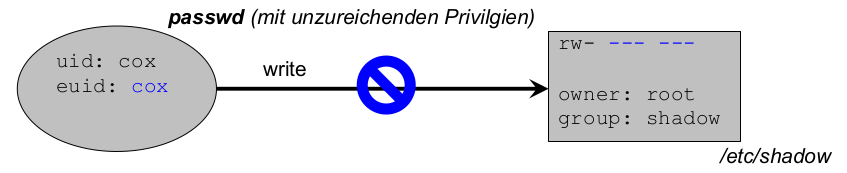
\includegraphics[width=\linewidth]{Assets/AdvancedOperatingSystems-passwd-problem.png}
        %\end{itemize*}
        \item
        Standard Linux Lösung:
        %\begin{itemize*}
        %\item \includegraphics[width=\linewidth]{Assets/AdvancedOperatingSystems-passwd-lösung.png}
        %\end{itemize*}
    \end{itemize*}

    \subsubsection{Modern: SELinux}

    \begin{itemize*}
        \item
        Ursprung
        \begin{itemize*}
            \item Anfang 2000er Jahre: sicherheitsfokussiertes Betriebssystemprojekt für US-amerikanische NSA {[}LoSm01{]}
            \item Implementierung des (eigentlich)$\mu$Kernel-Architekturkonzepts Flask
            \item heute: Open Source, Teil des mainline Linux Kernels
        \end{itemize*}
        \item
        Klassische UNIXoide: Sicherheitspolitik fest im Kernel implementiert
        \begin{itemize*}
            \item I-Nodes, PCBs, ACLs, UID, GID, SUID, ...
        \end{itemize*}
        \item
        Idee SELinux: Sicherheitspolitikals eigene BS-Abstraktion
        \begin{itemize*}
            \item zentrale Datenstruktur für Regeln, die erlaubte Zugriffe auf ein SELinux-System definiert
            \item erlaubt Modifikation und Anpassung an verschiedene Sicherheitsanforderungen $\rightarrow$ NFE Adaptivität ...
        \end{itemize*}
    \end{itemize*}


    \subparagraph{SELinux-Sicherheitsmechanismen}

    BS-Komponenten

    \begin{itemize*}
        \item
        Auswertung der Sicherheitspolitik: Security- Server , implementiert
        als Linux-Kernelmodul(Technik: LSM, Linux Security Module );
        $\rightarrow$ entscheidet über alle Zugriffe auf alle
        Objekte
        \item
        Durchsetzung der Sicherheitspolitik : LSM Hooks (generische
        Anfrage-Schnittstellen in allen BS-Funktionen)
        \item
        Administration der Sicherheitspolitik: geschrieben in Textform, muss
        zur Laufzeit in Security Server installiert werden
    \end{itemize*}

    %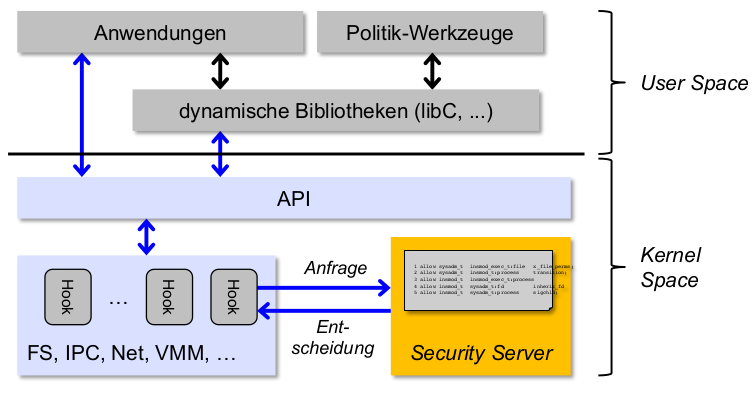
\includegraphics[width=\linewidth]{Assets/AdvancedOperatingSystems-selinux-security-server.png}

    %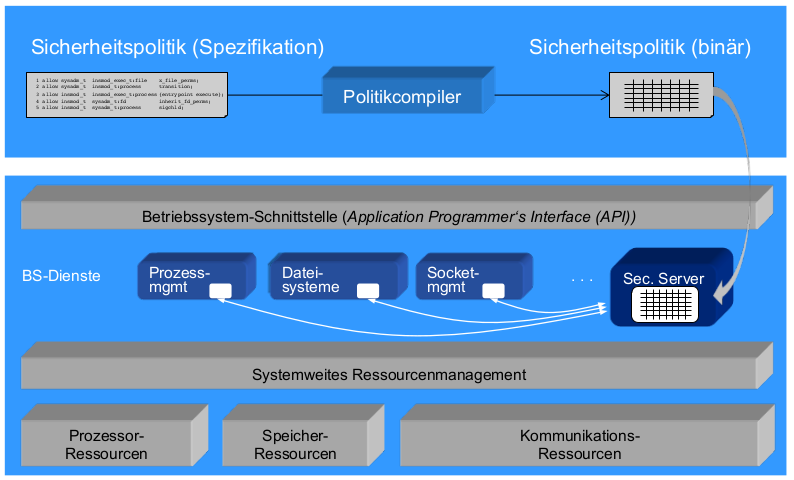
\includegraphics[width=\linewidth]{Assets/AdvancedOperatingSystems-selinux-sicherheitspolitik-installieren.png}


    \subparagraph{SELinux-Sicherheitspolitik}

    Repräsentation der Sicherheitspolitik:

    \begin{itemize*}
        \item
        physisch: in spezieller Datei, die alle Regeln enthält (in
        maschinenlesbarer Binärdarstellung), die der Kernel durchsetzen muss
        \item
        diese Datei wird aus Menge von Quelldateien in einer
        Spezifikationssprache für SELinux-Sicherheitspolitiken kompiliert
        \item
        diese ermöglicht anforderungsspezifische SELinux-Politiken: können
        (und müssen) sich von einem SELinux-System zum anderen wesentlich
        unterscheiden
        \item
        Politik wird während des Boot-Vorgangs in Kernel geladen
    \end{itemize*}


    \subparagraph{Politiksemantik}

    Regeln einer SELinux-Sicherheitspolitiken, Semantische
    Konzepte(Auswahl):

    \begin{itemize*}
        \item
        Type Enforcement (TE)
        \item
        Typisierung von
        \begin{itemize*}
            \item Subjekten: Prozesse
            \item Objekten der Klassen: Dateien, Sockets, EA-Geräteschnittstellen, ...
        \end{itemize*}
        \item
        Rechte delegation durch Retypisierung(vgl. Unix-SUID!)
        \item
        %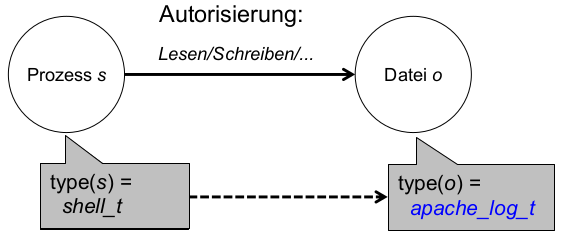
\includegraphics[width=\linewidth]{Assets/AdvancedOperatingSystems-selinux-retypisierung.png}
    \end{itemize*}


    \subparagraph{Autorisierungsinformationen}

    Security Context: Respräsentiert SELinux-Autorisierungsinformationen für
    jedes Objekt:

    %\begin{Shaded}
    %\begin{Highlighting}[]
    %\NormalTok{$ }\FunctionTok{ps}\NormalTok{ {-}Z}
    %\ExtensionTok{cox}\NormalTok{:doctor\_r:shell\_t:s0{-}s0:c0.c255 4056 pts/2 00:00:00 bash}
    %\NormalTok{$ }\FunctionTok{ls}\NormalTok{ {-}Z /etc/shadow}
    %\ExtensionTok{system\_u}\NormalTok{:object\_r:shadow\_t:s0 /etc/shadow}
    %\end{Highlighting}
    %\end{Shaded}

    \begin{itemize*}
        \item
        Semantik:
        \begin{itemize*}
            \item Prozess bash läuft (momentan) mit Typ \texttt{shell\_t}
            \item Datei shadow hat (momentan) den Typen \texttt{shadow\_t}.
        \end{itemize*}
    \end{itemize*}


    \subparagraph{Autorisierungsregeln}

    ... werden systemweit festgelegt in dessen Sicherheitspolitik
    ( $\rightarrow$ MAC):

    Access Vector Rules

    \begin{itemize*}
        \item
        definieren Autorisierungsregeln basierend auf Subjek-/Objekttypen
        \item
        Zugriffe müssen explizit gewährt werden ( default-deny )

        %\begin{Shaded}
        %\begin{Highlighting}[]
        %\ExtensionTok{allow}\NormalTok{ shell\_t passwd\_exec\_t : file \{ execute \};}
        %\ExtensionTok{allow}\NormalTok{ passwd\_t shadow\_t : file \{ read write \};}
        %\end{Highlighting}
        %\end{Shaded}
        \item
        Semantik: Erlaube( ''allow'' ) ...
        \begin{itemize*}
            \item jedem Prozess mit Typ \texttt{shell\_t}
            \item ausführenden Zugriff (benötigt die Berechtigung \texttt{\{execute\}}),
            \item auf Dateien (also Objekte der Klassefile)
            \item mit Typ \texttt{passwd\_exec\_t}.
        \end{itemize*}
    \end{itemize*}


    \subparagraph{Autorisierungsmechanismen: passwd
        Revisited}

    Klassischer Anwendungsfall für SELinux-TE: Passwort ändern

    Lösung: Retypisierung bei Ausführung

    \begin{itemize*}
        \item
        Prozess wechselt in einen aufgabenspezifischen Typ \texttt{passwd\_t}
        \item
        $\rightarrow$ massiv verringertes
        Missbrauchspotenzial!
        \item
        %\includegraphics[width=\linewidth]{Assets/AdvancedOperatingSystems-passwd-lösung2.png}
    \end{itemize*}


    \subparagraph{SELinux: weitere
        Politiksemantiken}

    \begin{itemize*}
        \item
        hier nur gezeigt: Überblick über TE
        \item
        außerdem relevant für SELinux-Politiken (und deren Administration...):
        \begin{itemize*}
            \item Einschränkung von erlaubten Typtransitionen (Welches Programm darf mit welchem Typ ausgeführt werden?)
            \item weitere Abstraktionsschicht: rollenbasierte Regeln (RBAC)
            \item $\rightarrow$ Schutz gegen nicht vertrauenswürdige Nutzer (vs. nvw. Software)
        \end{itemize*}
        \item
        Ergebnis:
        \begin{itemize*}
            \item \cmark extrem feingranulare, anwendungsspezifische Sicherheitspolitik zur Vermeidung von privilege escalation Angriffen
            \item \cmark obligatorische Durchsetzung ( $\rightarrow$ MAC, zusätzlich zu Standard-Unix-DAC)
            \item O Softwareentwicklung: Legacy-Linux-Anwendungen laufen ohne Einschränkung, jedoch
            \item \xmark Politikentwicklung und -administrationkomplex!
        \end{itemize*}
    \end{itemize*}


    \subparagraph{Weitere Informationen zu
        SELinux}

    $\rightarrow$ MAC-Mechanismen ala SELinux sind
    heutzutage in vielerlei Software bereits zu finden:

    \begin{itemize*}
        \item
        Datenbanksoftware (SEPostgreSQL)
        \item
        Betriebssysteme für mobile Geräte (FlaskDroid)
        \item
        sehr wahrscheinlich: zukünftige, sicherheitsorientierte BS...
    \end{itemize*}


    \subsection{Isolationsmechanismen}

    \begin{itemize*}
        \item
        bekannt: Isolationsmechanismen für robuste Betriebssysteme
        \begin{itemize*}
            \item strukturierte Programmierung
            \item Adressraumisolation
        \end{itemize*}
        \item
        nun: Isolationsmechanismen für sichere Betriebssysteme
        \begin{itemize*}
            \item all die obigen...
            \item kryptografische Hardwareunterstützung: Intel SGX Enclaves
            \item sprachbasiert: \begin{itemize*} \item streng typisierte Sprachen und \emph{managed code} : Microsoft Singularity {[}HLAA05{]} \item speichersichere Sprachen (Rust) + Adressraumisolation ($\mu$Kernel): \href{https://www.redox-os.org/}{RedoxOS} \end{itemize*}
            \item isolierte Laufzeitumgebungen: Virtualisierung (Kap. 6)
        \end{itemize*}
    \end{itemize*}


    \subparagraph{Intel SGX}

    \begin{itemize*}
        \item
        SGX: Software Guard Extensions {[}CoDe16{]}
        \item
        Ziel: Schutz von sicherheitskritischen Anwendungen durch vollständige,
        hardwarebasierte Isolation
        \item
        $\rightarrow$ strenggenommen kein BS-Mechanismus:
        Anwendungen müssen dem BS nicht mehr vertrauen! (AR-Schutz, Wechsel
        von Privilegierungsebenen, ...)
        \item
        Annahmen/Voraussetzungen:
        \begin{enumerate*}

            \item sämtliche Software nicht vertrauenswürdig (potenziell durch Angreifer kontrolliert)
            \item Kommunikation mit dem angegriffenen System nicht vertrauenswürdig (weder vertraulich noch verbindlich)
            \item kryptografische Algorithmen (Verschlüsselung und Signierung) sind vertrauenswürdig, also nicht für den Angreifer zu brechen
            \item Ziel der Isolation: Vertraulichkeit, Integrität und Authentizität(nicht Verfügbarkeit) von Anwendungen (Code) und den durch sie verarbeiteten Informationen
        \end{enumerate*}
    \end{itemize*}


    \subparagraph{Enclaves}

    \begin{itemize*}
        \item
        Idee: geschützter Speicherbereich für Teilmenge der Seiten (Code und
        Daten) einer Task: Enclave Page Cache (EPC)
        \item
        Prozessor (und nur dieser) ver-und entschlüsselt EPC-Seiten
        \item
        %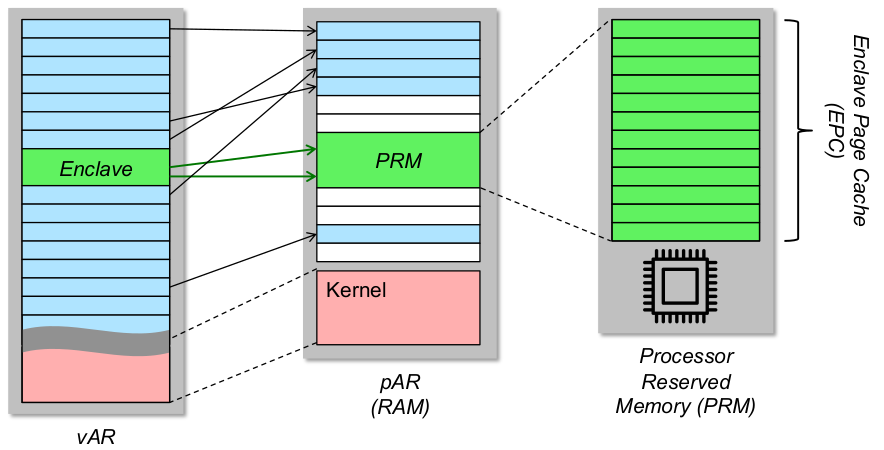
\includegraphics[width=\linewidth]{Assets/AdvancedOperatingSystems-SGX-enclaves.png}
        \item
        Enclaves: Erzeugung
        \begin{itemize*}
            \item Erzeugen: App. $\rightarrow$ Syscall $\rightarrow$ BS-Instruktion an CPU (ECREATE)
            \item Seiten hinzufügen: App. $\rightarrow$ Syscall $\rightarrow$ BS-Instruktion an CPU (EADD) \begin{itemize*} \item Metainformationen für jede hinzugefügte Seite als Teil der EPC-Datenstruktur (u.a.: Enklave - ID, Zugriffsrechte, vAR-Adresse) \end{itemize*}
            \item Initialisieren: App. $\rightarrow$ Syscall $\rightarrow$ BS-Instruktion an CPU (EINIT) \begin{itemize*} \item finalisiert gesamten Speicherinhalt für diese Enclave \item CPU erzeugt Hashwert = eindeutige Signatur des Enclave - Speicherinhalts \item falls BS bis zu diesem Punkt gegen Integrität der Anwendung verstoßen hat: durch Vergleich mit von dritter Seite generiertem Hashwert feststellbar! \end{itemize*}
        \end{itemize*}
        \item
        Enclave - Zustandsmodell (vereinfacht) :
        %\begin{itemize*}
        %\item 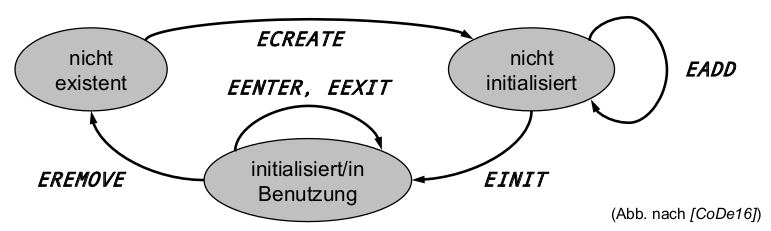
\includegraphics[width=\linewidth]{Assets/AdvancedOperatingSystems-SGX-enclaves-model.png}
        %\end{itemize*}
        \item
        Zugriff: App. $\rightarrow$ CPU-Instruktionen in User
        Mode (EENTER, EEXIT)
        \begin{itemize*}
            \item CPU erfordert, dass EPC-Seiten in vARder zugreifenden Task
            %\item
            % %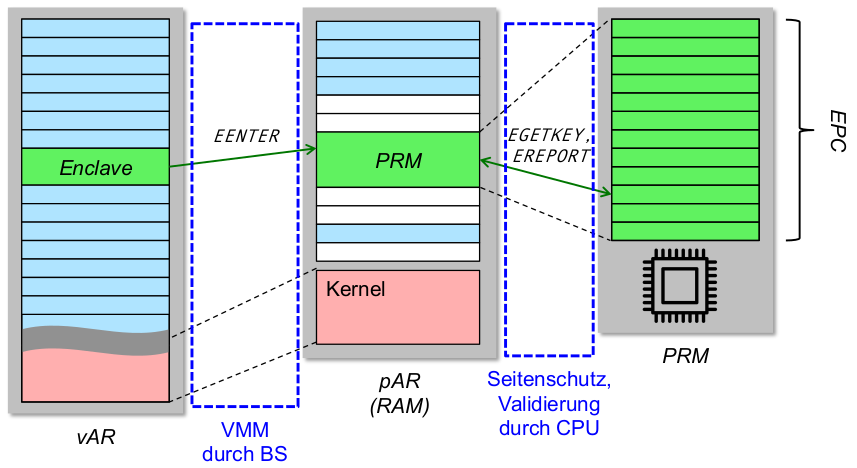
\includegraphics[width=\linewidth]{Assets/AdvancedOperatingSystems-SGX-enlaves-zugriff.png}
        \end{itemize*}
    \end{itemize*}


    \subparagraph{SGX: Licht und Schatten}

    \begin{itemize*}
        \item
        Einführung 2015 in Skylake - Mikroarchitektur
        \item
        seither in allen Modellen verbaut, jedoch nicht immer aktiviert
        \item
        Nutzer bislang: Demos und Forschungsprojekte, Unterstützung durch
        einige Cloud-Anbieter, (noch) keine größeren Märkte erschlossen
        \item
        Konzept hardwarebasierter Isolation ...
        \begin{itemize*}
            \item \cmark liefert erstmals die Möglichkeit zur Durchsetzung von Sicherheitspolitiken auf Anwendungsebene
            \item O setzt Vertrauen in korrekte (und nicht böswillige) Hardwarevoraus
            \item O Dokumentation und Entwicklerunterstützung (im Ausbau ...)
            \item \xmark schützt mittels Enclaves einzelne Anwendungen, aber nicht das System
            \item \xmark steckt hinsichtlich praktischer Eigenschaften noch in den Anfängen (vgl. $\mu$Kernel...): \begin{itemize*} \item Performanz {[}WeAK18{]} \item Speicherkapazität(max. Größe EPC: 128 MiB, davon nur 93 MiBnutzbar) \item $\rightarrow$ komplementäre NFE: Speichereffizienz! \end{itemize*}
        \end{itemize*}
    \end{itemize*}


    \subsection{Sicherheitsarchitekturen}

    Sicherheitsarchitektur... ist die Softwarearchitektur (Platzierung,
    Struktur und Interaktion) der Sicherheitsmechanismen eines IT-Systems.

    \begin{itemize*}
        \item
        Voraussetzung zum Verstehen jeder Sicherheitsarchitektur:
        \begin{itemize*}
            \item Verstehen des Referenzmonitorprinzips
            \item frühe Forschungen zu Betriebssystemsicherheit in 1970er-1980er Jahren durch US-Verteidigungsministerium
            \item Schlüsselveröffentlichung: Anderson-Report(1972){[}Ande72{]}
            \item $\rightarrow$ fundamentalen Eigenschaften zur Charakterisierung von Sicherheitsarchitekturen
        \end{itemize*}
        \item
        Begriffe des Referenzmonitorprinzips kennen wir schon:
        \begin{itemize*}
            \item Abgrenzung passiver Ressourcen (in Form einzelner Objekte, z.B. Dateien)
            \item von Subjekten (aktiven Elementen, z.B. laufenden Programmen, Prozessen) durch Betriebssystem
        \end{itemize*}
    \end{itemize*}


    \subsubsection{Referenzmonitorprinzip}

    \begin{itemize*}
        \item
        Idee:
        \begin{itemize*}
            \item $\rightarrow$ sämtliche Autorisierungsentscheidungen durch einen zentralen (abstrakten) Mechanismus = Referenzmonitor
            \item Bewertet jeden Zugriffsversuch eines Subjekts auf Objekt durch Anwendung einer Sicherheitspolitik (security policy) \begin{itemize*} \item $\rightarrow$ vgl. SELinux \end{itemize*}
            \item somit: Architekturbeschreibung, wie Zugriffe auf Ressourcen (z.B. Dateien) auf solche Zugriffe, die Sicherheitspolitik erlaubt, eingeschränkt werden
        \end{itemize*}
        \item
        Autorisierungsentscheidungen
        \begin{itemize*}
            \item basieren auf sicherheitsrelevanten Eigenschaften jedes Subjekts und jedes Objekts
            \item einige Beispiele kennen wir schon: \begin{itemize*} \item Nutzname, Unix-Gruppe \item Prozess-ID, INode-Nummer \item SELinux-Typ \end{itemize*}
        \end{itemize*}
        \item
        Architekturkomponenten in a nutshell:
        %\begin{itemize*}
        %\item 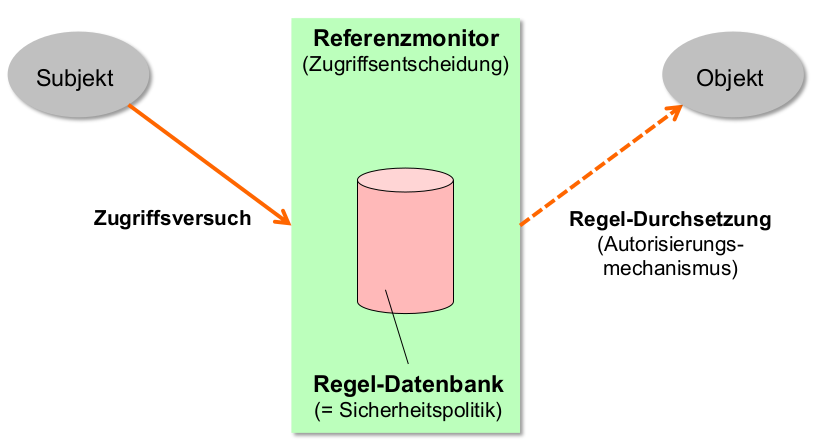
\includegraphics[width=\linewidth]{Assets/AdvancedOperatingSystems-Referenzmonitorprinzip.png}
        %\end{itemize*}
    \end{itemize*}

    Definierende Eigenschaften: Referenzmonitor ist eine
    Architekturkomponenten, die

    \begin{itemize*}
        \item
        (RM 1) bei sämtlichen Subjekt/Objekt-Interaktionen involviert sind
        \begin{itemize*}
            \item $\rightarrow$ Unumgehbarkeit ( total mediation )
        \end{itemize*}
        \item
        (RM 2) geschützt sind vor unautorisierter Manipulation
        \begin{itemize*}
            \item $\rightarrow$ Manipulationssicherheit ( tamperproofness )
        \end{itemize*}
        \item
        (RM 3) hinreichend klein und wohlstrukturiert sind, um formalen
        Analysemethoden zugänglich zu sein
        \begin{itemize*}
            \item $\rightarrow$ Verifizierbarkeit ( verifyability )
        \end{itemize*}
    \end{itemize*}


    \subparagraph{Referenzmonitor in
        Betriebssystemen}

    Nahezu alle Betriebssysteme implementieren irgendeine Form eines
    Referenzmonitors {[}Jaeg11{]} und können über Begriffe, wie

    \begin{itemize*}
        \item
        Subjekte
        \item
        Objekte
        \item
        Regeln einer Sicherheitspolitik charakterisiert sowie auf
        \item
        Unumgehbarkeit
        \item
        Manipulationssicherheit
        \item
        Verifizierbarkeit ihrer Sicherheitsarchitektur hin untersucht werden
    \end{itemize*}

    Beispiel: Standard- Linux

    \begin{itemize*}
        \item
        Subjekte (generell Prozesse)
        \begin{itemize*}
            \item haben reale (und effektive) Nutzer-Identifikatoren (UIDs)
        \end{itemize*}
        \item
        Objekte (verschiedene Systemressourcen, genutzt für Speicherung,
        Kommunikation: Dateien, Directories, Sockets, SharedMemory usw.)
        \begin{itemize*}
            \item haben ACLs (,,rwxrw-\/-\/-\/-'')
        \end{itemize*}
        \item
        Regeln der Sicherheitspolitik, die durch den Referenzmonitor (hier
        Kernel) unterstützt werden
        \begin{itemize*}
            \item hart codiert, starr
        \end{itemize*}
        \item
        Sicherheitsattribute, die durch diese Regeln zur Prüfung genutzt
        werden (z.B. Zugriffsmodi)
        \begin{itemize*}
            \item Objekten zugeordnet
            \item modifizierbar
        \end{itemize*}
    \end{itemize*}

    Man beurteile die Politikimplementierung in dieser Architektur bzgl.:

    \begin{itemize*}
        \item
        Unumgehbarkeit
        \item
        Manipulationssicherheit
        \item
        Verifizierbarkeit
    \end{itemize*}


    \subparagraph{Referenzmonitorimplementierung:
        Flask}

    ( Flask - Architekturmodell)

    %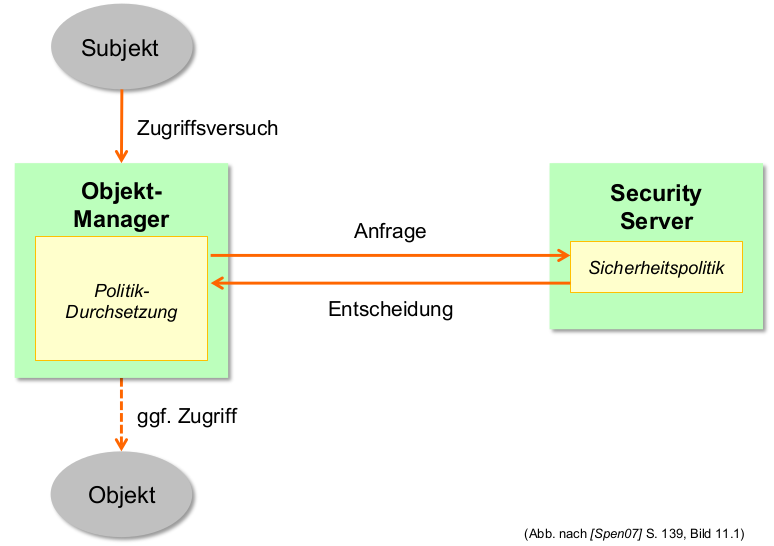
\includegraphics[width=\linewidth]{Assets/AdvancedOperatingSystems-referenzmonitor-flask.png}


    \subparagraph{SELinux-Architektur: Security
        Server}

    \begin{itemize*}
        \item
        Security Server: Laufzeitumgebung für Politik in Schutzdomäne des
        Kerns
        \item
        Objektmanager: implementiert in allen BS-Dienstenmittels,, Linux
        Security Module Framework ''
        \begin{itemize*}
            \item jedes Subsystemvon SELinux , das zuständig für \begin{enumerate*} \item Erzeugung neuer Objekte \item Zugriff auf existierende Objekte \end{enumerate*}
            \item Beispiele: \begin{enumerate*} \item Prozess-Verwaltung (behandelte Objekte: hauptsächlich Prozesse) \item Dateisystem (behandelte Objekte: hauptsächlich Dateien) \item Networking/Socket-Subsystem (behandelte Objekte: {[}verschiedene Typen von{]} Sockets) \item u.a. \end{enumerate*}
        \end{itemize*}
    \end{itemize*}

    SELinux-Architektur: Objektklassen

    \begin{itemize*}
        \item
        Objektmanager zur Verwaltung verschiedener Objektklassen
        \item
        spiegeln Diversität und Komplexität von Linux BS-Abtraktionen wider:
        \begin{itemize*}
            \item Dateisysteme: file, dir, fd, filesystem, ...
            \item Netzwerk: netif, socket, tcp\_socket, udp\_socket, ...
            \item IPC: msgq, sem, shm, ...
            \item Sonstige: process, system, ...
            \item ...
        \end{itemize*}
    \end{itemize*}

    Dateisystem als Objektmanager

    \begin{itemize*}
        \item
        Durch Analyse von Linux - Dateisystem und zugehöriger API wurden zu
        überwachenden Objektklassen identifiziert:
        \begin{itemize*}
            \item ergibt sich unmittelbar aus Linux-API: \begin{itemize*} \item Dateien \item Verzeichnisse \item Pipes \end{itemize*}
            \item feingranularere Objektklassen für durch Dateien repräsentierte Objekte (Unix-Prinzip: ,,everythingisa file''!): \begin{itemize*} \item reguläre Dateien \item symbolische Links \item zeichenorientierte Geräte \item blockorientierte Geräte \item FIFOs \item Unix-Domain Sockets (lokale Sockets) \end{itemize*}
        \end{itemize*}
        \item
        Permissions (Zugriffsrechte)
        \item
        für jede Objektklasse: Menge an Permissions definiert, um Zugriffe auf
        Objekte dieser Klasse zu kontrollieren
        \item
        Permissions: abgeleitet aus Dienstleistungen, die Linux-Dateisystem
        anbietet
        \item
        $\rightarrow$ Objektklassen gruppieren verschiedene
        Arten von Zugriffsoperationen auf verschiende Arten von Objekten
        \item
        z.B. Permissions für alle ,,Datei''-Objektklassen (Auswahl ...): read,
        write, append, create, execute, unlink
        \item
        für ,,Verzeichnis''-Objektklasse: add\_name, remove\_name, reparant,
        search, rmdir
    \end{itemize*}


    \subsubsection{Trusted Computing Base
        (TCB)}

    Begriff zur Bewertung von Referenzmonitorarchitekturen: TCB ( Trusted
    Computing Base )

    \begin{itemize*}
        \item
        = die Hard-und Softwarefunktionen eines IT-Systems, die notwendig und
        hinreichend sind, um alle Sicherheitsregeln durchzusetzen.
        \item
        besteht üblicherweise aus
        \begin{enumerate*}

            \item Laufzeitumgebung der Hardware(nicht E/A-Geräte)
            \item verschiedenen Komponenten des Betriebssystem-Kernels
            \item Benutzerprogrammen mit sicherheitsrelevanten Rechten (bei Standard-UNIX/Linux-Systemen: diejenigen mit root-Rechten)
        \end{enumerate*}
        \item
        Betriebssystemfunktionen, die Teil der TCB sein müssen, beinhalten
        Teile
        \begin{itemize*}
            \item des Prozessmanagements
            \item des Speichermanagements
            \item des Dateimanagements
            \item des E/A-Managements
            \item alle Referenzmonitorfunktionen
        \end{itemize*}
    \end{itemize*}


    \section{Echtzeitfähigkeit}


    \subsection{Motivation}

    Echtzeitbegriff: Was ist ein Echtzeitsystem?

    \begin{quote}
        Any system in which the time at which output is produced is significant.
        This is usually because the input corresponds to some movement in the
        physical world, and the output has to relate to that same movement. The
        lag from input time to output time must be sufficiently small for
        acceptable timeliness. (The Oxford DictionaryofComputing)
    \end{quote}

    \begin{quote}
        A real-time system is any information processing activity or system
        which has to respond to externally generated input stimuli within a
        finite and specified period. {[}Young 1982{]}
    \end{quote}

    \begin{quote}
        A real-time system is a system that is required to react to stimuli from
        the environment (including the passage of physical time) within time
        intervals dictated by the environment. {[}Randall et.al. 1995{]}
    \end{quote}

    Spektrum von Echtzeitsystemen:

    \begin{enumerate*}
        \item
        Regelungssysteme: z.B. eingebettete Systeme (exakter: Steuerungs-,
        Regelungs-u. Überwachungssysteme = ,,SRÜ''-Systeme)
        \item
        Endanwender-Rechnersysteme: z.B. Multimediasysteme
        \item
        Lebewesen: Menschen, Tiere
    \end{enumerate*}

    Beispiel Regelungssystem: ,,Fly-by-Wire''-Fluglage-Regelungssystem
    (Schema)

    \begin{enumerate*}
        \item
        Flugzeugbewegung
        \item
        Sensoren + Einstellmöglichkeiten des Piloten
        \item
        Echtzeit-Datenverarbeitung (durch Echtzeit-Rechnersystem)
        \item
        Aktoren setzen Berechnung um
        \item
        Einstellung von Regelflächen
        \item
        Aerodynamik und Flug Mechanik führt zu Flugzeugbewegung (1.)
    \end{enumerate*}

    Beispiel Überwachungssysteme

    \begin{itemize*}
        \item
        Luftraumüberwachung:
        \begin{itemize*}
            \item Ortsfeste Radarstation
            \item Mobile Radarstation
            \item Tiefflieger-Erfassungsradar
            \item Flugplatzradar Netzfunkstellen
            \item Zentrale
        \end{itemize*}
        \item
        Umweltüberwachung: Stickstoffdioxidkonzentration über Europa
        \item
        Vorgeburtliche Gesundheitsüberwachung: Herzschlagsüberwachungssystem
        für Mutter und Kind
    \end{itemize*}

    Beispiel Multimediasystem

    \begin{itemize*}
        \item
        zeitabhängige Datenwiedergabe
        \item
        Bildwiedergabe bei Mediendatenströmen
        \item
        Durchführung der Schritte durch Multimedia-Task binnen \$t\_\{i+1\} -
        t\_i\$
        \item
        Frist für Rendering in Multimedia-Tasks: festgelegt durch periodische
        Bildrate (24\textasciitilde48 fps $\rightarrow$ 1/24
        ... 1/48 s)
        \item
        $\rightarrow$ Berücksichtigung bei Scheduling,
        Interruptbehandlung, Speicherverwaltung, ... erforderlich!
    \end{itemize*}

    Zwischenfazit {[}Buttazzo97{]}

    \begin{itemize*}
        \item
        Murphy`s General Law: If something can go wrong, it will got wrong.
        \item
        Murphy`s Constant: Damage to an object is proportional to its value.
        \item
        Johnson`s First Law: If a system stops working, it will do it at the
        worst possible time.
        \item
        Sodd`sSecond Law: Sooner or later, the worst possible combination of
        circumstances will happen.
    \end{itemize*}

    Realisierung von Echtzeiteigenschaften: komplex und fragil!


    \subsection{Terminologie}

    bevor wir uns über Echtzeit-Betriebssystemen unterhalten:

    \begin{enumerate*}
        \item
        Wie ist die Eigenschaft Echtzeit definiert?
        \item
        Was sind (rechnerbasierte) Echtzeitsysteme?
        \item
        Wie können Echtzeitanwendungen beschrieben werden?
        \item
        Welche grundsätzlichen Typen von Echtzeitprozessen gibt es/wodurch
        werden diese charakterisiert?
    \end{enumerate*}

    Antwortzeit:

    \begin{itemize*}
        \item
        Alle Definitionen -die zitierten u. andere - betrachten eine
        ,,responsetime'' (Antwortzeit, Reaktionszeit) als das Zeitintervall,
        das ein System braucht, um (irgend)eine Ausgabe als Reaktion auf
        (irgend)eine Eingabe zu erzeugen.
    \end{itemize*}

    Frist

    \begin{itemize*}
        \item
        Bei Echtzeitsystemen ist genau dieses \$\textbackslash Delta t\$
        kritisch, d.h. je nach Art des Systems darf dieses auf keinen Fall zu
        groß werden.
        \item
        Genauer spezifizierbar wird dies durch Einführung einer Frist
        (deadline, due time) \$d\$, die angibt bis zu welchem Zeitpunkt
        spätestmöglich die Reaktion erfolgt sein muss, bzw. wie groß das
        Intervall \$\textbackslash Delta t\$ maximal sein darf.
    \end{itemize*}

    Echtzeitfähigkeit und Korrektheit

    \begin{itemize*}
        \item
        Wird genau dieses maximale Zeitintervall in die Spezifikation eines
        Systems einbezogen, bedeutet dies, dass ein Echtzeitsystem nur dann
        korrekt arbeitet, wenn seine Reaktion bis zur spezifizierten Frist
        erfolgt.
        \item
        Die Frist trennt also korrektes von inkorrektem Verhalten des Systems.
    \end{itemize*}

    %\includegraphics[width=\linewidth]{Assets/AdvancedOperatingSystems-echtzeitfähigkeit.png}

    Harte und weiche Echtzeitsysteme

    \begin{itemize*}
        \item
        Praktische Anwendungen erfordern oft Unterscheidung in harte und
        weiche Echtzeitsysteme:
        \begin{itemize*}
            \item hartes Echtzeitsystem: keine Frist darf jemals überschritten werden (sonst: katastrophale Konsequenzen)
            \item weiches Echtzeitsystem: maßvolles (im spezifizierten Maß) Überschreiten von Fristen tolerierbar
        \end{itemize*}
    \end{itemize*}


    \subsection{Charakteristika von
        Echtzeit-Prozessen}

    \begin{itemize*}
        \item
        reale Echtzeitanwendungen beinhalten periodische oder aperiodische
        Prozesse (oder Mischung aus beiden)
        \item
        typische Unterscheidung:
        \begin{itemize*}
            \item Periodische Prozesse \begin{itemize*} \item zeitgesteuert (typisch: periodische Sensorauswertung) \item oft: kritische Aktivitäten $\rightarrow$ harte Fristen \end{itemize*}
            \item Aperiodische Prozesse \begin{itemize*} \item ereignisgesteuert \item Abhängig von Anwendung: harte oder weiche Fristen, ggf. sogar Nicht-Echtzeit \end{itemize*}
        \end{itemize*}
    \end{itemize*}


    \subsubsection{Periodische Prozesse}

    \begin{itemize*}
        \item
        bei Echtzeit-Anwendungen: häufigster Fall
        \item
        typisch für:
        \begin{enumerate*}

            \item periodische Analyse von Sensor-Daten (z.B. Umweltüberwachung)
            \item Aktionsplanung (z.B. automatisierte Montage)
            \item Erzeugung oder Verarbeitung einzelner Dateneinheiten eines multimedialen Datenstroms
            \item ...
        \end{enumerate*}
        \item
        Prozessaktivierung
        \begin{itemize*}
            \item ereignisgesteuert oder zeitgesteuert
            \item Prozesse, die Eingangsdaten verarbeiten: meist ereignisgesteuert, z.B. wenn neues Datenpaket eingetroffen
            \item Prozesse, die Ausgangsdaten erzeugen: meist zeitgesteuert, z.B. Ansteuerung von Roboteraktoren
        \end{itemize*}
    \end{itemize*}

    Periodische Prozesse

    \begin{itemize*}
        \item
        Fristen:
        \begin{itemize*}
            \item hart oder weich (anwendungsabhängig) \begin{itemize*} \item innerhalb einer Anwendung sind sowohl Prozesse mit harten oder weichen Fristen möglich \item Frist: spätestens am Ende der aktuellen Periode, möglich auch frühere Frist \end{itemize*}
            %\item
            % %\includegraphics[width=\linewidth]{Assets/AdvancedOperatingSystems-echtzeit-periodisch-frist.png}
        \end{itemize*}
        \item
        Modellierung:
        \begin{itemize*}
            \item unendliche Folge identischer Aktivierungen: Instanzen, aktiviert mit konstanter Rate (Periode)
            %\item
            % %\includegraphics[width=\linewidth]{Assets/AdvancedOperatingSystems-echtzeit-periodisch-modellierung.png}
        \end{itemize*}
        \item
        Aufgaben des Betriebssystems:
        \begin{itemize*}
            \item WennalleSpezifikationeneingehaltenwerden-muss Betriebssystem garantieren, dass \begin{enumerate*} \item zeitgesteuerte periodische Prozesse: mit ihrer spezifizierten Rate aktiviert werden und ihre Frist einhalten können \item ereignisgesteuerte periodische Prozesse: ihre Frist einhalten können \end{enumerate*}
        \end{itemize*}
    \end{itemize*}


    \subsubsection{Aperiodische Prozesse}

    \begin{itemize*}
        \item
        typisch für
        \begin{itemize*}
            \item unregelmäßig auftretende Ereignisse, z.B.: \begin{itemize*} \item Überfahren der Spurgrenzen, Unterschreiten des Sicherheitsabstands $\rightarrow$ Reaktion des Fahrassistenzsystems \item Nutzereingaben in Multimediasystemen ( $\rightarrow$ Spielkonsole) \end{itemize*}
        \end{itemize*}
        \item
        Prozessaktivierung
        \begin{itemize*}
            \item ereignisgesteuert
        \end{itemize*}
        \item
        Fristen
        \begin{itemize*}
            \item oft weich(aber anwendungsabhängig)
        \end{itemize*}
        \item
        Aufgabendes Betriebssystems
        \begin{itemize*}
            \item bei Einhaltung der Prozessspezifikationen muss Betriebssystem auch hier für Einhaltung der Fristen sorgen
        \end{itemize*}
        \item
        Modellierung
        \begin{itemize*}
            \item bestehen ebenfalls aus (maximal unendlicher) Folge identischer Aktivierungen (Instanzen); aber: Aktivierungszeitpunkte nicht regelmäßig (möglich: nur genau eine Aktivierung)
            %\item
            % %\includegraphics[width=\linewidth]{Assets/AdvancedOperatingSystems-echtzeit-aperiodisch-modellierung.png}
        \end{itemize*}
    \end{itemize*}


    \subsubsection{Parameter von
        Echtzeit-Prozessen}

    \begin{itemize*}
        \item
        %\includegraphics[width=\linewidth]{Assets/AdvancedOperatingSystems-echtzeit-parameter-instanz.png}
        \item
        \$a\_i\$: Ankunftszeitpunkt (arrival time); auch r ... request
        time/release time
        \begin{itemize*}
            \item Zeitpunkt, zu dem ein Prozess ablauffähig wird
        \end{itemize*}
        \item
        \$s\_i\$: Startzeitpunkt (start time)
        \begin{itemize*}
            \item Zeitpunkt, zu dem ein Prozess mit der Ausführung beginnt
        \end{itemize*}
        \item
        \$f\_i\$: Beendigungszeitpunkt (finishing time)
        \begin{itemize*}
            \item Zeitpunkt, an dem ein Prozess seine Ausführung beendet
        \end{itemize*}
        \item
        \$d\_i\$: Frist (deadline, due time)
        \begin{itemize*}
            \item Zeitpunkt, zu dem ein Prozess seine Ausführung spätestens beenden sollte
        \end{itemize*}
        \item
        \$C\_i\$: Bearbeitungszeit(bedarf) (computation time)
        \begin{itemize*}
            \item Zeitquantum, das Prozessor zur vollständigen Bearbeitung der aktuellen Instanz benötigt (Unterbrechungen nicht eingerechnet)
        \end{itemize*}
        \item
        %\includegraphics[width=\linewidth]{Assets/AdvancedOperatingSystems-echtzeit-parameter-instanz2.png}
        \item
        \$L\_i\$: Unpünktlichkeit (lateness): \$L\_i= f\_i - d\_i\$
        \begin{itemize*}
            \item Zeitbetrag, um den ein Prozess früher oder später als seine Frist beendet wird (wenn Prozess vor seiner Frist beendet, hat \$L\_i\$ negativen Wert)
        \end{itemize*}
        \item
        \$E\_i\$: Verspätung (exceeding time, tardiness): \$E\_i= max(0,
        L\_i)\$
        \begin{itemize*}
            \item Zeitbetrag, den ein Prozess noch nach seiner Frist aktiv ist
        \end{itemize*}
        \item
        %\includegraphics[width=\linewidth]{Assets/AdvancedOperatingSystems-echtzeit-parameter-instanz3.png}
        \item
        \$X\_i\$: Spielraum (Laxity, Slacktime): \$X\_i = d\_i - a\_i - C\_i\$
        \begin{itemize*}
            \item maximales Zeitquantum, um das Ausführung eines Prozesses verzögert werden kann, damit dieser noch bis zu seiner Frist beendet werden kann (\$f\_i=d\_i\$)
        \end{itemize*}
        \item
        außerdem:
        \begin{itemize*}
            \item criticality: Parameter zur Beschreibung der Konsequenzen einer Fristüberschreitung (typischerweise ,,hart'' oder ,,weich'')
            \item \$V\_i\$ ...Wert (value): Parameter zum Ausdruck der relativen Wichtigkeit eines Prozesses bezogen auf andere Prozesse der gleichen Anwendung
        \end{itemize*}
    \end{itemize*}


    \subsection{Echtzeitfähige
        Betriebssysteme}

    \begin{itemize*}
        \item
        Hauptfragestellungen
        \begin{enumerate*}

            \item Was muss BS zu tun, um Echtzeitprozesse zu ermöglichen? Welche Teilprobleme müssen beachtet werden?
            \item Welche Mechanismen müssen hierfür anders als bei nicht-echtzeitfähigen Betriebssystemen implementiert werden, und wie?
        \end{enumerate*}
        \item
        Grundlegender Gedanke
        \begin{itemize*}
            \item Abgeleitet aus den Aufgaben eines Betriebssystems sind folgende Fragestellungenvon Interesse:
        \end{itemize*}
        \begin{enumerate*}

            \item Wie müssen die Ressourcen verwaltet werden? ( $\rightarrow$ CPU, Speicher, E/A, ...)
            \item Sind neue Abstraktionen, Paradigmen (Herangehensweisen) und entsprechende Komponenten erforderlich (oder günstig)?
        \end{enumerate*}
        \item
        Prozess-Metainformationen
        \begin{enumerate*}

            \item Frist
            \item Periodendauer
            \item abgeleitet davon: Spielraum, Unpünktlichkeit, Verspätung, ...
            \item im Zusammenhang damit: Prioritätsumkehr, Überlast
        \end{enumerate*}
        \item
        Ressourcen-Management
        \begin{itemize*}
            \item Wie müssen Ressourcen verwaltet werden, damit Fristen eingehalten werden können?
        \end{itemize*}
    \end{itemize*}

    Wir betrachten i.F.

    \begin{enumerate*}
        \item
        Algorithmen, die Rechnersysteme echtzeitfähig machen -einschließlich
        des Betriebssystems:
        \begin{itemize*}
            \item grundlegende Algorithmen zum Echtzeitscheduling
            \item Besonderheiten der Interruptbehandlung
            \item Besonderheiten der Speicherverwaltung
        \end{itemize*}
        \item
        Probleme, die behandelt werden müssen, um Echtzeitfähigkeit nicht zu
        be- oder verhindern:
        \begin{itemize*}
            \item Prioritätsumkehr
            \item Überlast
            \item Kommunikation-und Synchronisationsprobleme
        \end{itemize*}
    \end{enumerate*}


    \subsubsection{Echtzeitscheduling}

    \begin{itemize*}
        \item
        Scheduling:
        \begin{itemize*}
            \item Schedulingvon Prozessen/Threads als wichtigster Einflussfaktor auf Zeitverhalten des Gesamtsystems
        \end{itemize*}
        \item
        Echtzeit-Scheduling:
        \begin{itemize*}
            \item benötigt: Scheduling-Algorithmen, die Scheduling unter Berücksichtigung der ( unterschiedlichen ) Fristen der Prozesse durchführen können
        \end{itemize*}
        \item
        Fundamentale Algorithmen:
        \begin{itemize*}
            \item wichtigste Strategien:
        \end{itemize*}
        \begin{enumerate*}

            \item Ratenmonotones Scheduling (RM)
            \item Earliest Deadline First (EDF)
        \end{enumerate*}
        \begin{itemize*}
            \item beide schon 1973 von Liu \& Layland ausführlich diskutiert {[}Liu\&Layland73{]}
        \end{itemize*}
    \end{itemize*}

    Annahmen der Scheduling-Strategien

    \begin{itemize*}
        \item
        A1: Alle Instanzen eines periodischen Prozesses \$t\_i\$ treten
        regelmäßig und mit konstanter Rate auf (= werden aktiviert ). Das
        Zeitintervall \$T\_i\$ zwischen zwei aufeinanderfolgenden
        Aktivierungen heißt Periode des Prozesses.
        \item
        A2: Alle Instanzen eines periodischen Prozesses \$t\_i\$ haben den
        gleichen Worst-Case-Rechenzeitbedarf \$C\_i\$.
        \item
        A3: Alle Instanzen eines periodischen Prozesses \$t\_i\$ haben die
        gleiche relative Frist \$D\_i\$, welche gleich der Periodendauer
        \$T\_i\$ ist.
        \item
        A4: Alle Prozessesind kausal unabhängig voneinander (d.h. keine
        Vorrang- und Betriebsmittel-Restriktionen)
        \item
        A5: Kein Prozess kann sich selbst suspendieren, z.B. bei
        E/A-Operationen.
        \item
        A6: Alle Prozesse werden mit ihrer Aktivierung sofort rechenbereit (
        release time = arrival time ).
        \item
        A7: Jeglicher Betriebssystem-Overhead (Kontextwechsel,
        Scheduler-Rechenzeit) wird vernachlässigt.
    \end{itemize*}

    A5-7 sind weitere Annahmen des Scheduling Modells

    Ratenmonotones Scheduling (RM)

    \begin{itemize*}
        \item
        Voraussetzung:
        \begin{itemize*}
            \item periodisches Bereitwerden der Prozesse/Threads, d.h. periodische Prozesse bzw. Threads
        \end{itemize*}
        \item
        Strategie RM:
        \begin{itemize*}
            \item Prozess (Thread) mit höchster Ankunftsrate bekommt höchste statische Priorität (Kriterium: Wie oft pro Zeiteinheit wird Prozess bereit?)
            \item Scheduling-Zeitpunkt: nur einmal zu Beginn (bzw. wenn neuer periodischer Prozess auftritt)
            \item präemptiver Algorithmus
        \end{itemize*}
        \item
        %\includegraphics[width=\linewidth]{Assets/AdvancedOperatingSystems-echtzeit-scheduling-rm.png}
        \begin{itemize*}
            \item Zuteilung eines Prozessors nach RM
            \item \$t\_1, t\_2\$: Anforderungen von Prozessorzeit durch zwei periodische Prozesse
            \item darunter: Prozessorzuteilung nach RM
        \end{itemize*}
        \item
        Optimalität von RM
        \begin{itemize*}
            \item Unter allen Verfahren mit festen (statischen)Prioritäten ist RM optimaler Algorithmus in dem Sinne, dass kein anderes Verfahren dieser Klasse eine Prozessmenge einplanen kann, die nicht auch von RM geplant werden kann. {[}Liu\&Layland73{]}
        \end{itemize*}
        \item
        Prozessor-Auslastungsfaktor
        \begin{itemize*}
            \item Bei gegebener Menge von n periodischen Prozessen gilt: \$U=\textbackslash sum\_\{i=1\}\^{}n \textbackslash frac\{C\_i\}\{T\_i\}\$
            \item mit \$\textbackslash frac\{C\_i\}\{T\_i\}\$ Anteil an Prozessorzeit für jeden periodischen Prozess \$t\_i\$
            \item und \$U\$ Summe der Prozessorzeit zur Ausführung der gesamten Prozessmenge (,,utilization factor'')
        \end{itemize*}
        \item
        Prozessorlast
        \begin{itemize*}
            \item \$U\$ ist folglich Maß für die durch Prozessmenge verursachte Last am Prozessor $\rightarrow$ Auslastungsfaktor
        \end{itemize*}
        \item
        Planbarkeitsanalyse einer Prozessmenge
        \begin{itemize*}
            \item im allgemeinen Fall kann RM einen Prozessor nicht zu 100\% auslasten
            \item von besonderem Interesse: kleinste obere Grenze des Auslastungsfaktors \$U\_\{lub\}\$ (lub: ,,least upper bound'')
        \end{itemize*}
        \item
        Beispiel für \$n=2\$
        \begin{itemize*}
            %\item
            % %\includegraphics[width=\linewidth]{Assets/AdvancedOperatingSystems-echtzeit-scheduling-rm2.png}
            \item Obere Grenze des Prozessor-Auslastungsfaktors für zwei periodische Prozesse als Funktion des Verhältnisses ihrer Perioden.
            \item (Abb. nach {[}Buttazzo97{]} Bild 4.7, S. 90)
        \end{itemize*}
        \item
        Obere Auslastungsgrenze bei RM
        \begin{itemize*}
            \item nach {[}Buttazzo97{]} (S. 89-91) erhält man bei n Prozessen für RM: \$U\_\{lub\}=n(2\^{}\{\textbackslash frac\{1\}\{n\}\}-1)\$
            \item für \$n\textbackslash rightarrow\textbackslash infty\$ konvergiert \$U\_\{lub\}\$ zu \$ln\textbackslash{} 2 \textbackslash approx 0,6931...\$
            \item Wird genannter Wert nicht überschritten, sind beliebige Prozessmengen planbar.
            \item (Herleitung siehe {[}Buttazzo97{]} , Kap. 4.3.3)
        \end{itemize*}
    \end{itemize*}


    \subsubsection{Earliest Deadline First (EDF)}
    \begin{itemize*}
        \item Voraussetzung:
        \begin{itemize*}
            \item kann sowohl periodische als auch aperiodische Prozesse planen
        \end{itemize*}
        \item Optimalität:
        \begin{itemize*}
            \item EDF in Klasse der Schedulingverfahren mit dynamischen Prioritäten: optimaler Algorithmus {[}Liu\&Layland73{]}
        \end{itemize*}
        \item Strategie EDF:
        \begin{itemize*}
            \item Zu jedem Zeitpunkt erhält Prozess mit frühester Frist höchste dynamische Priorität
            \item Scheduling-Zeitpunkt: Bereitwerden eines (beliebigen) Prozesses
            \item präemptiver Algorithmus (keine Verdrängung bei gleichen Prioritäten)
        \end{itemize*}
        \item Beispiel
        \begin{itemize*}
            %\item \includegraphics[width=\linewidth]{Assets/AdvancedOperatingSystems-echtzeit-scheduling-edf.png}
            \item Zuteilung eines Prozessors nach EDF
            \item \$t\_1, t\_2\$: Anforderungen nach Prozessorzeit durch zwei periodische Prozesse
            \item darunter: Prozessorzuteilung nach EDF
        \end{itemize*}
        \item Planbarkeitsanalyse:
        \begin{itemize*}
            \item Mit den Regeln \$A1 ... A7\$ ergibt sich für die obere Schranke des Prozessorauslastungsfaktors: \$U\_\{lub\}= 1\textbackslash rightarrow\$ Auslastung bis 100\% möglich!
            \item Eine Menge periodischer Prozesse ist demnach mit EDF planbar genau dann wenn: \$U=\textbackslash sum\_\{i=1\}\^{}n \textbackslash frac\{C\_i\}\{T\_i\}\textbackslash leq 1\$ (Prozessor natürlich nicht mehr als 100\% auslastbar)
        \end{itemize*}
        \item Beweis: Obere Auslastungsgrenze bei EDF
        \begin{itemize*}
            \item Behauptung: Jede Menge von n periodischen Tasks ist mit EDF planbar $\leftrightarrow$: \$U=\textbackslash sum\_\{i=1\}\^{}n \textbackslash frac\{C\_i\}\{T\_i\}\textbackslash leq 1\$
            \item $\leftarrow$: \$U\textgreater1\$ übersteigt die verfügbare Prozessorzeit; folglich kann niemals eine Prozessmenge mit dieser (oder höherer) Gesamtauslastung planbar sein.
            \item $\rightarrow$: Beweis durch Widerspruch. Annahme: \$U\textbackslash leq 1\$ und die Prozessmenge ist nicht planbar. Dies führt zu einem Schedule mit Fristverletzung zu einem Zeitpunkt \$t\_2\$, z.B.:
            %\begin{itemize*} \item \includegraphics[width=\linewidth]{Assets/AdvancedOperatingSystems-echtzeit-scheduling-edf2.png} \end{itemize*}
            \item Beobachtungen an diesem Schedule:
            \begin{itemize*}
                \item \$exists\$ ein längstes, kontinuierliches Rechenintervall \${[}t\_1,t\_2{]}\$, in welchem nur Prozessinstanzen mit Fristen \$\textbackslash leq t\_2\$ rechnen
                \item die Gesamtrechenzeit \$C\_\{bad\}\$ aller Prozesse in \${[}t\_1,t\_2{]}\$ muss die verfügbare Prozessorzeit übersteigen: \$C\_\{bad\} \textgreater{} t\_2-t\_1\$ (sonst: keine Fristverletzung an \$t\_2\$)
                \item Anwesenheit in \${[}t\_1,t\_2{]}\$ leitet sich davon ab, ob (genauer: wie oft) die Periode eines Prozesses in \$t\_2-t\_1\$ passt: \$t\_i\$ in \${[}t\_1,t\_2{]}\textbackslash Leftrightarrow\textbackslash lfloor\textbackslash frac\{t\_2-t\_1\}\{T\_i\}\textbackslash rfloor \textgreater0\$
                \item Damit ist \$C\_\{bad\}\$ die Summe der Rechenzeiten aller Prozessinstanzen, die garantiert in \${[}t\_1,t\_2{]}\$ sind, mithin: \$C\_\{bad\}=\textbackslash sum\_\{i=1\}\^{}n \textbackslash lfloor\textbackslash frac\{t\_2-t\_1\}\{T\_i\}\textbackslash rfloor C\_i\$
                \item Im Beispiel: \$t\_1... t\_3\$ in \${[}t\_1,t\_2{]}\$, folglich: \$C\_\{bad\}= 2 C\_1 + 1 C\_2 + 1 C\_3\$
                \item Zu zeigen: Beobachtung \$C\_\{bad\}\textgreater{} t\_2-t\_1\$ widerspricht Annahme \$U\textbackslash leq 1\$.
                \item Es gilt \$\textbackslash sum\_\{i=1\}\^{}n \textbackslash lfloor\textbackslash frac\{t\_2-t\_1\}\{T\_i\}\textbackslash rfloor C\_i\textbackslash leq\textbackslash sum\_\{i=1\}\^{}n\textbackslash frac\{t\_2-t\_1\}\{T\_i\}C\_i\$ wegen Abrundung.
                \item Mit \$U=\textbackslash sum\_\{i=1\}\^{}n\textbackslash frac\{C\_i\}\{T\_i\}\$ folgt daraus \$C\_\{bad\}\textbackslash leq(t\_2-t\_1)U\$
                \item \$C\_\{bad\}\textgreater t\_2-t\_1\$ entspricht also \$(t\_2-t\_1)U\textgreater t\_2-t\_1\$ und somit \$U\textgreater1\$. Widerspruch zur Annahme!
            \end{itemize*}
        \end{itemize*}
    \end{itemize*}


    \subsubsection{Vergleich: EDF vs. RM}
    %\includegraphics[width=\linewidth]{Assets/AdvancedOperatingSystems-echtzeit-edf-vs-rm.png}

    Zuteilung eines Prozessors nach EDF (dynamisch) bzw. RM (statisch)
    \$t\_1,t\_2\$: Anforderungen nach Prozessorzeit durch zwei periodische
    Prozesse darunter: Prozessorzuteilung nach EDF bzw. RM

    \begin{itemize*}
        \item
        gut erkennbar: deutliche Unterschiede bei Scheduling mit statischem
        (RM) vs. dynamischem Algorithmus (EDF).
    \end{itemize*}

    Vergleich: Anzahl Prozesswechsel

    \begin{itemize*}
        \item
        Häufigkeit von Prozesswechseln im Beispiel:
        \begin{itemize*}
            \item RM: 16
            \item EDF: 12
        \end{itemize*}
        \item
        Ursache: dynamische Prioritätenvergabe führt dazu, dass Instanz II von
        \$t\_2\$ die gleiche Priorität wie Instanz A von \$t\_1\$ hat (usw.)
        $\rightarrow$ keine unnötige Verdrängung
    \end{itemize*}

    Vergleich: 100\% Prozessorauslastung

    \begin{itemize*}
        \item
        EDF: erzeugt auch bei Prozessorauslastung bis 100\% (immer) korrekte
        Schedules
        \item
        RM: kann das im allgemeinen Fall nicht
        \item
        Bedeutung von 100\% Prozessorauslastung in der Praxis: Überwiegend
        müssen Systeme mit harten Echtzeitanforderungen auch weiche Echtzeit-
        sowie Nicht-Echtzeit-Prozesse unterstützen. Daher: Belegungslücken am
        Prozessor für die letzteren beiden nutzbar.
    \end{itemize*}

    Vergleich: Implementierung

    \begin{itemize*}
        \item
        RM
        \begin{itemize*}
            \item statisch: jeweils eine Warteschlange pro Priorität:
            \item Einfügen und Entfernen von Tasks: \$O(1)\$
            %\item
            % %\includegraphics[width=\linewidth]{Assets/AdvancedOperatingSystems-echtzeit-scheduling-rm-statisch.png}
        \end{itemize*}
        \item
        EDF
        \begin{itemize*}
            \item dynamisch: balancierter Binärbaum zur Sortierung nach Prioritäten:
            \item Einfügen und Entfernen von Tasks: \$O(log\textbackslash{} n)\$
            %\item
            % %\includegraphics[width=\linewidth]{Assets/AdvancedOperatingSystems-echtzeit-scheduling-edf-dynamisch.png}
        \end{itemize*}
    \end{itemize*}

    Scheduling in Multimedia-Anwendungen

    \begin{itemize*}
        \item
        Konkretisierung des Betrachtungswinkels
        \begin{itemize*}
            \item RM und EDF wurden entwickelt insbesondere für Echtzeit-Regelsysteme $\rightarrow$ ohne Berücksichtigung von Multimediasystemen
            \item Multimediasysteme $\rightarrow$ andere Probleme, schwächere Annahmen: spezialisierte Scheduling-Algorithmen
            \item gehen meist auch von EDF und/oder RM als Grundlage aus
        \end{itemize*}
        \item
        Betrachteter Algorithmus:
        \begin{itemize*}
            \item Beispielfür spezialisierten Scheduling-Algorithmus: \begin{itemize*} \item RC-Algorithmus - entwickelt an University of Texas \item Anpassung von EDF an Charakteristika von Multimedia-Anwendungen \end{itemize*}
        \end{itemize*}
    \end{itemize*}

    Prozesstypen in Multimedia-Anwendungen

    \begin{enumerate*}
        \item
        Echte Multimedia-Prozesse
    \end{enumerate*}

    \begin{itemize*}
        \item
        periodische Prozesse: weiche Fristen
        \begin{enumerate*}

            \item pünktliche periodische Prozesse mit konstantem Prozessorzeitbedarf \$C\$ für jede Instanz (unkomprimierte Audio- und Videodaten)
            \item pünktliche periodische Prozesse mit unterschiedlichem \$C\$ einzelner Instanzen (komprimierte Audio- und Videodaten)
            \item unpünktliche periodische Prozesse: \begin{itemize*} \item verspätete Prozesse \item verfrühte Prozesse \end{itemize*}
        \end{enumerate*}
        \item
        aperiodische-Prozesse aus Multimedia-Anwendungen: weiche Fristen
    \end{itemize*}

    \begin{enumerate*}
        \setcounter{enumi}{1}
        \item
        Prozesse nebenläufiger Nicht-Multimedia-Anwendungen
        \begin{itemize*}
            \item interaktive Prozesse : keine Fristen , aber: keine zu langen Antwortzeiten Ansatz (z.B.): maximal tolerierbare Verzögerung
            \item Hintergrund-Prozesse : zeitunkritisch, keine Fristen, aber : dürfen nicht verhungern
        \end{itemize*}
    \end{enumerate*}

    Multimediaanwendungen sind ein typisches Beispiel für mögliche
    Abweichungen der Lastpezifikation \$(T\_i,C\_i)\$ eines
    Echtzeitprozesses!

    Problem: Abweichungen von Lastspezifikation

    \begin{itemize*}
        \item
        gibt Prozessor nicht frei
        \item
        verspätete periodische Prozesse
    \end{itemize*}


    \subsubsection{RC Algorithmus}

    \begin{itemize*}
        \item
        Ziel
        \begin{itemize*}
            \item spezifikationstreue Prozesse nicht bestrafen durch Fristüberschreitung aufgrund abweichender Prozesse
        \end{itemize*}
        \item
        Idee
        \begin{itemize*}
            \item grundsätzlich: Schedulingnach frühester Fristaufsteigend (= EDF) $\rightarrow$ für eine vollständig spezifikationstreue Prozessmenge verhält sich RC wie reines EDF
            \item Frist einer Instanz wird dynamisch angepasst:basierend auf derjenigen Periode, in der sie eigentlich sein sollte lt. Spezifikation der Prozessornutzung (\$U\_i\$, hier: ,,Rate''): \$U\_i=\textbackslash frac\{C\_i\}\{T\_i\}\$
            \item Bsp.: \$U\_i =\textbackslash frac\{20\}\{40\}=\textbackslash frac\{1\}\{2\}\$ (\$t\_B\$ hat spezifizierte Aktivitätsrate von \$0,5\$ pro Periode)
        \end{itemize*}
    \end{itemize*}


    \paragraph{RC Algorithmus: Strategie}

    \begin{itemize*}
        \item
        Variablen
        \begin{itemize*}
            \item \$a\_i\$: Ankunftszeit der zuletzt bereitgewordenen Instanz von \$t\_i\$
            \item \$t\_i\^{}\{virt\}\$: virtuelle Zeit in aktueller Periode, die \$t\_i\$ bereits verbraucht hat
            \item \$c\_i\^{}\{virt\}\$: Netto-Rechenzeit, die \$t\_i\$ in aktueller Periode bereits verbraucht hat
            \item \$d\_i\$: dynamische Frist von \$t\_i\$, nach der sich dessen Priorität berechnet (EDF)
        \end{itemize*}
        \item
        Strategie
        \begin{itemize*}
            \item für eine bereite (lauffähige) Instanz von \$t\_i\$: adaptiere dynamisch \$d\_i\$ basierend auf \$t\_i\^{}\{virt\}\$
            \item für eine bereit gewordene (neu angekommene oder zuvor blockierte) Instanzvon \$t\_i\$: aktualisiere \$t\_i\^{}\{virt\}\$ auf akt. Systemzeit \$(t)\textbackslash rightarrow\$ etwaiger ''Zeitkredit'' verfällt
        \end{itemize*}
    \end{itemize*}


    \paragraph{RC Algorithmus: Berechnung von
    \$t\_i\^{}\{virt\}\$}

    Beispiel: Situation bei \$t=20ms\$
    %\includegraphics[width=\linewidth]{Assets/AdvancedOperatingSystems-rc-ti-berechnen-1.png}

    Da \$t\_B\$ aber noch weiteren Rechenbedarf hat: Situation bei \$t=30
    ms\$
    %\includegraphics[width=\linewidth]{Assets/AdvancedOperatingSystems-rc-ti-berechnen-2.png}


    \paragraph{RC Algorithmus:
        Adaptionsfunktion}

    Für Prozess ti zu jedem Scheduling-Zeitpunkt:

    %\begin{Shaded}
    %\begin{Highlighting}[]
    %\NormalTok{RC (t\_i) \{}
    % \ControlFlowTok{if}\NormalTok{ (t\_i. status wurde auf BEREIT gesetzt) \{}
    %\NormalTok{ t\_i\^{}virt := max( t\_i\^{}virt , t ); }\CommentTok{//kein Zeitkredit {-}\textgreater{} kein ,,Nachholen\textquotesingle{}\textquotesingle{} von verpassten/ungenutzten Perioden}
    %\NormalTok{ \} }\ControlFlowTok{else}\NormalTok{ \{}
    %\NormalTok{ c\_i\^{}virt := Gesamtprozessorzeit seit letztem Aufruf RC(t\_i);}
    %\NormalTok{ t\_i\^{}virt := t\_i\^{}virt + c\_i\^{}virt / U\_i ; }\CommentTok{//Zeitwert, bis zu dem t\_i Rechenzeit gemäß seiner Rate U\_i erhalten hat}
    %\NormalTok{ \}}
    % \ControlFlowTok{if}\NormalTok{ (t\_i. status != BLOCKIERT) \{}
    %\NormalTok{ finde k, so dass gilt:}
    %\NormalTok{ a\_i + (k {-} }\DecValTok{1}\NormalTok{) * T\_i \textless{}= t\_i\^{}virt \textless{} a\_i + k * T\_i ; }\CommentTok{// finde diejenige (aktuelle oder zukünftige) Periode, in der t\_i\^{}virt liegt}
    %\NormalTok{ d\_i := a\_i + k * T\_i ; }\CommentTok{// setze d\_i auf deren Periodenende}
    %\NormalTok{ \}}
    %\NormalTok{\}}
    %\end{Highlighting}
    %\end{Shaded}


    \paragraph{RC Algorithmus: Scheduling}

    Zeitpunkte, zu denen der Scheduler aktiv wird:

    \begin{enumerate*}
        \item
        aktuell laufender Prozess \$t\_i\$ blockiert:
        \begin{itemize*}
            \item \$RC(t\_i)\$
        \end{itemize*}
        \item
        Prozesse \$t\_i...\_j\$ werden bereit:
        \begin{itemize*}
            \item \$for\textbackslash{} x\textbackslash in{[}i,j{]}: RC(t\_x)\$
        \end{itemize*}
        \item
        periodischer ,,clock tick'' (SchedulingInterrupt):
        \begin{itemize*}
            \item \$t\_i\$ := aktuell ausgeführter Prozess
            \item \$RC(t\_i)\$
        \end{itemize*}
    \end{enumerate*}

    anschließendes Scheduling (präemptiv) = EDF:

    %\begin{Shaded}
    %\begin{Highlighting}[]
    %\NormalTok{SCHED := \{t\_i |t\_i.status == BEREIT ⋀ d\_i minimal \}; }\CommentTok{// bereite(r) Prozess(e) mit nächster Frist}
    %\ControlFlowTok{if}\NormalTok{ (∃ t\_j : t\_j.status == LAUFEND) ⋀ ( d\_j ≤ d\_i )}
    % \ControlFlowTok{do}\NormalTok{ nothing; }\CommentTok{// ggf. laufenden Prozess bevorzugen}
    %\ControlFlowTok{else}
    %\NormalTok{ preempt(rnd\_member( SCHED )); }\CommentTok{// sonst: irgendein Prozess mit nächster Frist verdrängt den laufenden}
    %\end{Highlighting}
    %\end{Shaded}


    \paragraph{Umgang mit abweichenden Prozessen unter
        RC}

    %\includegraphics[width=\linewidth]{Assets/AdvancedOperatingSystems-rc-abweichende-prozesse.png}


    \paragraph{Resultat}

    \begin{quote}
        Garantie: Prozesse, die sich entsprechend ihrer Spezifikation verhalten,
        erhalten bis zum Ende jeder spezifizierten Periode ihren spezifizierten
        Anteil an Prozessorzeit.
    \end{quote}

    Auswirkung auf verschiedene Prozesstypen:

    \begin{itemize*}
        \item
        ,,pünktliche'' Prozesse: Einhaltung der Frist in jeder Periode
        garantiert (unabhängig von Verhalten anderer Prozesse)
        \item
        ,,verspätete'' Prozesse: nur aktuelle Periode betrachtet, Nachholen
        ,,ausgelassener Perioden'' nicht möglich
        \item
        ,,gierige'' Prozesse: Prozessorentzug, sobald andere lauffähige
        Prozesse frühere Fristen aufweisen
        \item
        nicht-periodische Hintergrundprozesse: pro ,,Periode'' wird
        spezifizierte Prozessorrate garantiert (z.B. kleine Raten bei großen
        ,,Periodendauern'' wählen.)
    \end{itemize*}


    \subsubsection{Umgang mit gemischten
        Prozessmengen}

    \begin{itemize*}
        \item
        Hintergrund-Scheduling:
        \begin{itemize*}
            \item Prinzip: %\includegraphics[width=\linewidth]{Assets/AdvancedOperatingSystems-gemischte-prozessmenge.png}
            \item rechenbereite Prozesse auf 2 Warteschlangen aufgeteilt (einfache Variante eines Mehr-Ebenen-Scheduling )
            \item Warteschlange 1: \begin{itemize*} \item alle periodischen Prozesse \item mit höchster Priorität mittels RM oder EDF bedient \end{itemize*}
            \item Warteschlange 2: \begin{itemize*} \item alle aperiodischen Prozesse \item nur bedient, wenn keine wartenden Prozesse in Warteschlange 1 \end{itemize*}
        \end{itemize*}
    \end{itemize*}


    \paragraph{Hintergrund-Scheduling: Vor- und
        Nachteile}

    \begin{itemize*}
        \item
        Hauptvorteil:
        \begin{itemize*}
            \item einfache Implementierung
        \end{itemize*}
        \item
        Nachteile:
        \begin{itemize*}
            \item Antwortzeit \textbf{aperiodischer Prozesse} kann zu lang werden (insbesondere bei hoher aperiodischer Last) $\rightarrow$ Verhungern möglich!
            \item geeignet nur für relativ zeitunkritische aperiodische Prozesse
        \end{itemize*}
        \item
        Beispiel: Hintergrund-Scheduling mit RM
        %\begin{itemize*}
        %\item \includegraphics[width=\linewidth]{Assets/AdvancedOperatingSystems-hintergrund-scheduling.png}
        %\end{itemize*}
    \end{itemize*}


    \paragraph{Optimierung:
        Server-Prozess}

    \begin{itemize*}
        \item
        Scheduling mit Server-Prozessen:
        \begin{itemize*}
            \item Prinzip: periodisch aktivierter Prozess benutzt zur Ausführung aperiodischer Prozessoranforderungen
            \item Beschreibung Server-Prozess: durch Parameter äquivalent zu wirklichem periodischen Prozess: \begin{itemize*} \item Periodendauer \$T\_S\$ \item ,,Prozessorzeitbedarf'' \$C\_S\$; jetzt Kapazitätdes Server-Prozesses \end{itemize*}
            \item Arbeitsweise Server-Prozess: \begin{itemize*} \item geplant mit gleichem Scheduling-Algorithmus wie periodische Prozesse \item zum Aktivierungszeitpunkt vorliegende aperiodische Anforderungen bedient bis zur Kapazität des Servers \item keine aperiodischen Anforderungen: Server suspendiert sich bis Beginn der nächsten Periode (Schedule wird ohne ihn weitergeführt $\rightarrow$ Prozessorzeit für periodische Prozesse) \item Kapazitätin jeder Server-Periode neu ''aufgeladen'' \end{itemize*}
        \end{itemize*}
    \end{itemize*}


    \paragraph{Beispiel: Server-Prozess mit
        RM}

    %\includegraphics[width=\linewidth]{Assets/AdvancedOperatingSystems-rm-server-prozess.png}


    \paragraph{Optimierung:
        Slack-Stealing}

    \begin{itemize*}
        \item
        Prinzip: Es existiert passiver Prozess ,,slack stealer'' (kein
        periodischer Server)
        \item
        versucht so viel Zeit wie möglich für aperiodische Anforderungen zu
        sammeln
        \item
        realisiert durch ,,slackstealing''(= Spielraum-Stehlen) bei
        periodischen Prozessen
        \item
        letztere auf Zeit-Achse so weit nach hinten geschoben, dass Frist und
        Beendigungszeitpunkt zusammenfallen
        \item
        Sinnvoll, da normalerweise Beenden periodischer Prozesse vor ihrer
        Frist keinerlei Vorteile bringt
        \item
        Resultat: Verbesserung der Antwortzeiten für aperiodische
        Anforderungen
        \item
        %\includegraphics[width=\linewidth]{Assets/AdvancedOperatingSystems-slack-stealing.png}
    \end{itemize*}


    \subsubsection{Prioritätsumkehr}

    \begin{quote}
        Mechanismen zur Synchronisation und Koordination sind häufige Ursachen
        für kausale Abhängigkeiten zwischen Prozessen!
    \end{quote}


    \paragraph{Problem}

    \begin{itemize*}
        \item
        Prinzip \emph{kritischer Abschnitt} (Grundlagen BS):
        \begin{itemize*}
            \item Sperrmechanismen stellen wechselseitigen Ausschluss bei der Benutzung exklusiver Betriebsmittel durch nebenläufige Prozesse sicher
            \item Benutzung von exklusiven sowie nichtentziehbaren Betriebsmitteln: kritischer Abschnitt
            \item Folge: Wenn ein Prozess einen kritischen Abschnitt betreten hat, darf er aus diesem nicht verdrängt werden (durch anderen Prozess, der dasselbe Betriebsmittel nutzen will)
        \end{itemize*}
        \item
        Konflikt: kritische Abschnitte vs. Echtzeit-Prioritäten
        \begin{itemize*}
            \item Falls ein weiterer Prozess mit höherer Priorität ablauffähig wird und im gleichen kritischen Abschnitt arbeiten will, muss er warten bis niederpriorisierter Prozess kritischen Abschnitt verlassen hat
            \item (zeitweise) Prioritätsumkehr möglich! d.h. aus einer (Teil-) Menge von Prozessen muss derjenige mit höchster Priorität auf solche mit niedrigerer Priorität warten
        \end{itemize*}
    \end{itemize*}


    \paragraph{Ursache der
        Prioritätsumkehr}

    \begin{itemize*}
        \item
        %\includegraphics[width=\linewidth]{Assets/AdvancedOperatingSystems-prioritätsumkehr-ursache.png}
        \item
        Prioritätsumkehr bei Blockierung an nichtentziehbarem, exklusivem
        Betriebsmittel
        \item
        $\rightarrow$ unvermeidlich
    \end{itemize*}


    \paragraph{Folgen der
        Prioritätsumkehr}

    \begin{itemize*}
        \item
        Kritisch bei zusätzlichen Prozessen mittlerer Priorität
        \item
        %\includegraphics[width=\linewidth]{Assets/AdvancedOperatingSystems-prioritätsumkehr-folgen.png}
        \item
        Lösung: Priority Inheritance Protocol (PIP)
    \end{itemize*}


    \paragraph{Lösung:
        Prioritätsvererbung}

    \begin{itemize*}
        \item
        !{[}Abb. nach {[}Buttazzo97{]} , Bild 7.6, S.188{]}
        \item
        ePrio ... effektive Priorität
    \end{itemize*}


    \subsubsection{Überlast}

    \begin{itemize*}
        \item
        Definition: kritische Situation - bei der die benötigte Menge an
        Prozessorzeit die Kapazität des vorhandenen Prozessors übersteigt
        \$(U\textgreater1)\$
        \begin{itemize*}
            \item Folge: nicht alle Prozesse können Fristen einhalten
        \end{itemize*}
        \item
        Hauptrisiko: kritische Prozesse können Fristen nicht einhalten
        $\rightarrow$ Gefährdung funktionaler und anderer
        nichtfkt. Eigenschaften ( $\rightarrow$ harte Fristen!)
        \item
        Stichwort: ,,graceful degradation'' (,,würdevolle'' Verschlechterung)
        statt unkontrollierbarer Situation $\rightarrow$
        Wahrung von Determinismus
    \end{itemize*}


    \paragraph{Wichtigkeit eines
        Prozesses}

    \begin{itemize*}
        \item
        Minimallösung: (lebenswichtig für Echtzeit-System)
        \begin{itemize*}
            \item Unterscheidung zwischen Zeitbeschränkungen (Fristen) und tatsächlicher Wichtigkeit eines Prozesses für System
        \end{itemize*}
        \item
        Allgemein gilt:
        \begin{itemize*}
            \item Wichtigkeit eines Prozesses ist unabhängig von seiner Periodendauer und irgendwelchen Fristen
            \item z.B. kann ein Prozess trotz späterer Frist viel wichtiger als anderer mit früherer Frist sein.
            \item Beispiel: Bei chemischem Prozess könnte Temperaturauswertung jede 10s wichtiger sein als Aktualisierung graphischer Darstellung an Nutzerkonsole jeweils nach 5s
        \end{itemize*}
    \end{itemize*}


    \paragraph{Umgang mit Überlast: alltägliche
        Analogien}

    \begin{enumerate*}
        \item
        Weglassen weniger wichtiger Aktionen
        \begin{itemize*}
            \item ohne Frühstück aus dem Haus...
            \item kein Zähneputzen ...
            \item Wichtung vom Problem bzw. Aktivitätsträgern (hier: Personen) abhängig!
        \end{itemize*}
        \item
        Verkürzen von Aktivitäten
        \begin{itemize*}
            \item Katzenwäsche...
        \end{itemize*}
        \item
        Kombinieren
        \begin{itemize*}
            \item kein Frühstück + Katzenwäsche + ungekämmt
        \end{itemize*}
    \end{enumerate*}


    \paragraph{Wichtung von Prozessen}

    Behandlung:

    \begin{itemize*}
        \item
        zusätzlicher Parameter V (Wert) für jeden Prozess/Thread einer
        Anwendung
        \item
        spezifiziert relative Wichtigkeit eines Prozesses (od. Thread) im
        Verhältnis zu anderen Prozessen (Threads) der gleichen Anwendung
        \item
        bei Scheduling: V stellt zusätzliche Randbedingung (primär: Priorität
        aufgrund von Frist, sekundär: Wichtigkeit)
    \end{itemize*}


    \paragraph{Obligatorischer und optionaler
        Prozessanteil}

    \begin{itemize*}
        \item
        Aufteilung der Gesamtberechnung \$(C\_\{ges\})\$ eines Prozesses in
        zwei Phasen
        \item
        einfache Möglichkeit der Nutzung des Konzepts des anpassbaren
        Prozessorzeitbedarfs
        \item
        Prinzip:
        \begin{itemize*}
            \item Bearbeitungszeitbedarf eines Prozesses zerlegt in \begin{enumerate*} \item obligatorischer Teil (Pflichtteil, \$C\_\{ob\}\$): muss unbedingt u. immer ausgeführt werden $\rightarrow$ liefert bedingt akzeptables Ergebnis \item optionaler Teil \$(C\_\{opt\})\$: nur bei ausreichender Prozessorkapazität ausgeführt $\rightarrow$ verbessert durch obligatorischen Teil erzieltes Ergebnis \end{enumerate*}
            \item Prinzip in unterschiedlicher Weise verfeinerbar
        \end{itemize*}
        \item
        %\includegraphics[width=\linewidth]{Assets/AdvancedOperatingSystems-obligatorisch-optionaler-prozessanteil.png}
    \end{itemize*}


    \subsubsection{Echtzeit-Interruptbehandlung}

    \begin{enumerate*}
        \item
        Fristüberschreitung durch ungeeignete Interruptbearbeitung
        %\begin{itemize*}
        %\item \includegraphics[width=\linewidth]{Assets/AdvancedOperatingSystems-interruptbehandlung-fristüberschreitung.png}
        %\end{itemize*}
        \item
        Lösung für Echtzeitsysteme ohne Fristüberschreitung
        \begin{itemize*}
            \item Interrupt wird zunächst nur registriert (deterministischer Zeitaufwand)
            \item tatsächliche Bearbeitung der Interruptroutine muss durch Scheduler eingeplant werden $\rightarrow$ Pop-up Thread
            %\item
            % %\includegraphics[width=\linewidth]{Assets/AdvancedOperatingSystems-interruptbehandlung-lösung.png}
        \end{itemize*}
    \end{enumerate*}


    \subsubsection{Echtzeit-Speicherverwaltung}

    \begin{itemize*}
        \item
        Prinzip:
        \begin{itemize*}
            \item Hauptanliegen: auch hier Fristen einhalten
            \item wie bei Interrupt-Bearbeitung und Prioritätsumkehr: unkontrollierbare Verzögerungen der Prozessbearbeitung (= zeitlicher Nichtdeterminismus) vermeiden!
        \end{itemize*}
        \item
        Ressourcenzuordnung, deswegen:
        \begin{enumerate*}

            \item keine Ressourcen-Zuordnung ,,on-demand'' (d.h. in dem Moment, wo sie benötigt werden) sondern ,,Pre-Allokation'' (= Vorab-Zuordnung)
            \item keine dynamische Ressourcenzuordnung (z.B. Hauptspeicher), sondern Zuordnung maximal benötigter Menge bei Pre-Allokation ( $\rightarrow$ BS mit ausschließlich statischer Hauptspeicherallokation: TinyOS)
        \end{enumerate*}
    \end{itemize*}


    \paragraph{Hauptspeicherverwaltung}

    \begin{itemize*}
        \item
        bei Anwendung existierender Paging-Systeme
        \begin{itemize*}
            \item durch unkontrolliertes Ein-/Auslagern ,,zeitkritischer'' Seiten (-inhalte): unkontrollierbare Zeitverzögerungen möglich!
            \item Technik hier: ,,Festnageln'' von Seiten im Speicher (Pinning, Memory Locking)
        \end{itemize*}
    \end{itemize*}


    \paragraph{Sekundärspeicherverwaltung}

    \begin{itemize*}
        \item
        Beispiel 1: FCFS Festplattenscheduling
        \begin{itemize*}
            \item Anforderungsreihenfolge = 98, 183, 37, 122, 14, 124, 65, 67
            \item Zuletzt gelesener Block: 53
            %\item
            % %\includegraphics[width=\linewidth]{Assets/AdvancedOperatingSystems-sekundärspeicherverwaltung-fcfs.png}
        \end{itemize*}
        \item
        Beispiel 2: EDF Festplattenscheduling
        \begin{itemize*}
            \item Anforderungsreihenfolge \$t\_1 = 98, 37, 124, 65\$
            \item Anforderungsreihenfolge \$t\_2 = 183, 122, 14, 67\$
            \item Zuletzt gelesener Block: 53 \textbar{} \textbar{} \$a\_i\$ \textbar{} \$d\_i\$ \textbar{} \textbar{} -\/-\/-\/-\/- \textbar{} -\/-\/-\/-\/- \textbar{} -\/-\/-\/-\/- \textbar{} \textbar{} \$t\_1\$ \textbar{} 0 \textbar{} 3 \textbar{} \textbar{} \$t\_2\$ \textbar{} 0 \textbar{} 9 \textbar{}
            %\item
            % %\includegraphics[width=\linewidth]{Assets/AdvancedOperatingSystems-sekundärspeicherverwaltung-edf.png}
        \end{itemize*}
        \item
        Primärziel: Wahrung der Echtzeitgarantien
        \begin{itemize*}
            \item naheliegend: EA-Schedulingnach Fristen $\rightarrow$ EDF (wie Prozessor)
            \item für Zugriffsreihenfolge auf Datenblöcke: lediglich deren Fristen maßgebend (weitere Regeln existieren nicht!)
        \end{itemize*}
        \item
        Resultat bei HDDs:
        \begin{itemize*}
            \item ineffiziente Bewegungen der Lese-/Schreibköpfe -ähnlich FCFS
            \item nichtdeterministische Positionierzeiten
            \item geringer Durchsatz
        \end{itemize*}
        \item
        Fazit:
        \begin{itemize*}
            \item Echtzeit-Festplattenscheduling $\rightarrow$ Kompromiss zwischen Zeitbeschränkungen und Effizienz
        \end{itemize*}
        \item
        bekannte Lösungen:
        \begin{enumerate*}

            \item Modifikation von EDF
            \item Kombination von EDF mit anderen Zugriffsstrategien
        \end{enumerate*}
    \end{itemize*}

    $\rightarrow$ realisierte Strategien:

    \begin{enumerate*}
        \item
        SCAN-EDF (SCAN: Kopfbewegung nur in eine Richtung bis
        Mitte-/Randzylinder; EDF über alle angefragten Blöcke \emph{in dieser
            Richtung} )
        \item
        Group Sweeping\_ (SCAN mit nach Fristen gruppenweiser Bedienung)
        \item
        Mischstrategien
    \end{enumerate*}

    \begin{itemize*}
        \item
        Vereinfachung:
        \begin{itemize*}
            \item o.g. Algorithmen i.d.R. zylinderorientiert $\rightarrow$ berücksichtigen bei Optimierung nur Positionierzeiten (Grund: Positionierzeit meist $>>$ Latenzzeit)
            %\item
            % %\includegraphics[width=\linewidth]{Assets/AdvancedOperatingSystems-sekundärspeicherverwaltung-festplatte.png}
        \end{itemize*}
    \end{itemize*}


    \subsubsection{Kommunikation und
        Synchronisation}

    \begin{itemize*}
        \item
        zeitlichen Nichtdeterminismus vermeiden:
        \begin{enumerate*}

            \item Interprozess-Kommunikation
        \end{enumerate*}
        \begin{itemize*}
            \item Minimierung blockierender Kommunikationsoperationen
            \item indirekte Kommunikation $\rightarrow$ CAB zum Geschwindigkeitsausgleich
            \item keine FIFO-Ordnungen (nach Fristen priorisieren)
            \item CAB ... Cyclic Asynchronous Buffer: %\includegraphics[width=\linewidth]{Assets/AdvancedOperatingSystems-kommunikation-cab.png}
        \end{itemize*}
        \begin{enumerate*}

            \setcounter{enumi}{1}
            \item Synchronisation
        \end{enumerate*}
        \begin{itemize*}
            \item keine FIFO-Ordnungen, z.B. bei Semaphor-Warteschlangen (vgl. o.)
        \end{itemize*}
    \end{itemize*}


    \paragraph{Cyclic Asynchronous Buffer
        (CAB)}

    Kommunikation zwischen 1 Sender und n Empfängern:

    \begin{itemize*}
        \item
        nach erstem Schreibzugriff: garantiert niemals undefinierte
        Wartezeiten durch Blockierung von Sender/Empfänger
        \item
        Lesen/Überschreiben in zyklischer Reihenfolge:
        %\begin{itemize*}
        %\item \includegraphics[width=\linewidth]{Assets/AdvancedOperatingSystems-kommunikation-zyklisch-cab.png}
        %\end{itemize*}
        \item
        Implementierung:
        \begin{itemize*}
            \item MRW: Most-Recently-Written; Zeiger auf jüngstes, durch Sender vollständig geschriebenes Element
            \item LRW: Least-Recently-Written; Zeiger auf ältestes durch Sender geschriebenes Element
            \item Garantien: \begin{itemize*} \item sowohl \emph{MRW} als auch \emph{LRW} können ausschließlich durch Sender manipuliert werden $\rightarrow$ keine inkonsistenten Zeiger durch konkurrierende Schreibzugriffe! \item sowohl \emph{MRW} als auch \emph{LRW} zeigen niemals auf ein Element, das gerade geschrieben wird $\rightarrow$ keine inkonsistenten Inhalte durch konkurrierende Schreib-/Lesezugriffe! \end{itemize*}
            \item Regeln für Sender: \begin{itemize*} \item muss \textbf{nach} jedem Schreiben \emph{MRW} auf geschriebenes Element setzen \item muss \textbf{bevor} \emph{LRW} geschrieben wird \emph{LRW} inkrementieren \end{itemize*}
            \item Regel für Empfänger: muss immer nach Lesen von \emph{MRW} als nächstes \emph{LRW} anstelle des Listennachbarn lesen
        \end{itemize*}
        \item
        Sender-Regeln:
        \begin{itemize*}
            \item anschaulich, ohne aktiven Empfänger
            %\item
            % %\includegraphics[width=\linewidth]{Assets/AdvancedOperatingSystems-cab-sender-regel.png}
        \end{itemize*}
        \item
        Empfänger-Regel:
        \begin{itemize*}
            \item anschaulich, ohne aktiven Sender
            %\item
            % %\includegraphics[width=\linewidth]{Assets/AdvancedOperatingSystems-cab-empfänger.png}
        \end{itemize*}
    \end{itemize*}

    Sonderfall 1: Empfänger schneller als Sender

    \begin{itemize*}
        \item
        nach Zugriff auf MRW muss auf Lesesequenz bei LRW fortgesetzt werden
        $\rightarrow$ transparenter Umgang mit nicht-vollem
        Puffer
        \item
        Abschwächung der Ordnungsgarantien:Empfänger weiß nur, dass Aktualität
        der Daten zwischen LRW und MRW liegt
        \item
        Empfänger (nach min. einem geschriebenen Element) niemals durch leeren
        Puffer blockiert
        \item
        %\includegraphics[width=\linewidth]{Assets/AdvancedOperatingSystems-cab-sonderfall-1.png}
    \end{itemize*}

    Sonderfall 2: Sender schneller als Empfänger

    \begin{itemize*}
        \item
        Schreiben in Puffer grundsätzlich in Reihenfolge der Elemente
        $\rightarrow$ keine blockierenden Puffergrenzen
        $\rightarrow$ niemals Blockierung des Senders
        \item
        keine Vollständigkeitsgarantien:Empfänger kann nicht sicher sein, eine
        temporal stetige Sequenz zu lesen
        \item
        $\rightarrow$ Szenarien, in denen Empfänger sowieso
        nur an aktuellsten Daten interessiert (z.B. Sensorwerte)
        \item
        %\includegraphics[width=\linewidth]{Assets/AdvancedOperatingSystems-cab-sonderfall-2.png}
    \end{itemize*}

    Konkurrierende Zugriffe:

    \begin{itemize*}
        \item
        ... sind durch Empfänger immer unschädlich (da lesend)
        \item
        ... müssen vom Sender nach Inkrementieren von LRW nicht-blockierend
        erkannt werden (klassisches Semaphormodell ungeeignet)
        \item
        schnellerer Sender überspringtein gesperrtes Element durch erneutes
        Inkrementieren von LRW , muss MRW trotzdem nachziehen
        \item
        %\includegraphics[width=\linewidth]{Assets/AdvancedOperatingSystems-cab-konkurrierende-zugriffe.png}
    \end{itemize*}


    \subsection{Architekturen und
        Beispiel-Betriebssysteme}

    \begin{itemize*}
        \item
        Architekturprinzipien:
        \begin{itemize*}
            \item müssen Echtzeitmechanismen unterstützen; ermöglicht entsprechende Strategien zur Entwicklungs-oder Laufzeit (CPU-Scheduler, EA-Scheduler, IPC ...)
            \item müssen funktional geringe Komplexität aufweisen $\rightarrow$ theoretische und praktische Beherrschung von Nichtdeterminismus \begin{itemize*} \item Theoretisch: Modellierung und Analyse (vgl. Annahmen für Scheduling-Planbarkeitsanalyse) \item Praktisch: Implementierung (vgl. RC-Scheduler, Prioritätsvererbung) \end{itemize*}
        \end{itemize*}
        \item
        Konsequenzen:
        \begin{itemize*}
            \item Architekturen für komplementäre NFE: \begin{itemize*} \item Sparsamkeit $\rightarrow$ hardwarespezifische Kernelimplementierung \item Adaptivität $\rightarrow$ $\mu$Kernel, Exokernel \end{itemize*}
            \item zu vermeiden: \begin{itemize*} \item starke Hardwareabstraktion $\rightarrow$ Virtualisierungsarchitekturen \item Kommunikation und Synchronisationskosten $\rightarrow$ verteilte BS \item Hardwareunabhängigkeit und Portabilität $\rightarrow$ vgl. Mach \end{itemize*}
        \end{itemize*}
    \end{itemize*}

    Auswahl: Beispiel-Betriebssysteme

    \begin{itemize*}
        \item
        wir kennen schon:
        \begin{itemize*}
            \item funktional kleine Kernelimplementierung: TinyOS
            \item hardwarespezifischer $\mu$Kernel: L4-Abkömmlinge
            \item Mischung aus beidem: RIOT
            \item Kommerziell bedeutender $\mu$Kernel: QNX Neutrino
        \end{itemize*}
        \item
        weitere Vertreter:
        \begin{itemize*}
            \item hardwarespezifische Makrokernel: VRTX, VxWorks
            \item $\mu$Kernel: DRYOS, DROPS
            \item ,,Exokernel'' ...?
        \end{itemize*}
    \end{itemize*}

    VRTX (Versatile Real-Time Executive)

    \begin{itemize*}
        \item
        Entwickler:
        \begin{itemize*}
            \item Hunter \& Ready
        \end{itemize*}
        \item
        Eckdaten:
        \begin{itemize*}
            \item Makrokernel
            \item war erstes kommerzielles Echtzeitbetriebssystem für eingebettete Systeme
            \item heutige Bedeutung eher historisch
            \item Nachfolger (1993 bis heute): Nucleus RTOS (Siemens)
        \end{itemize*}
        \item
        Anwendung:
        \begin{itemize*}
            \item Eingebettete Systeme in Automobilen(Brems-und ABS-Controller)
            \item Mobiltelefone
            \item Geldautomaten
        \end{itemize*}
        \item
        Einsatzgebiete
        \begin{itemize*}
            \item spektakulär: im Hubble-Weltraumteleskop
        \end{itemize*}
    \end{itemize*}

    VxWorks

    \begin{itemize*}
        \item
        Entwickler:
        \begin{itemize*}
            \item Wind River Systems (USA)
        \end{itemize*}
        \item
        Eckdaten:
        \begin{itemize*}
            \item modularer Makrokernel
            \item Konkurrenzprodukt zu VRTX
            \item Erfolgsfaktor: POSIX-konforme API
            \item ähnlich QNX: ,,skalierbarer'' Kernel,zuschneidbarauf Anwendungsdomäne ( $\rightarrow$ Adaptivitätsansatz)
        \end{itemize*}
        \item
        Anwendung:
        \begin{itemize*}
            \item eingebettete Systeme:
            \item industrielle Robotersteuerung
            \item Luft-und Raumfahrt
            \item Unterhaltungselektronik
        \end{itemize*}
        \item
        Einsatzgebiete
        \begin{itemize*}
            \item Deep-Impact-Mission zur Untersuchung des Kometen Temple 1
            \item NASA Mars Rover
            \item SpaceX Dragon
        \end{itemize*}
    \end{itemize*}

    DRYOS®

    \begin{itemize*}
        \item
        Entwickler: Canon Inc.
        \item
        Eckdaten:
        \begin{itemize*}
            \item Mikrokernel(Größe: 16 kB)
            \item Echtzeit-Middleware (Gerätetreiber $\rightarrow$ Objektive)
            \item Anwendungen: AE-und AF-Steuerung/-Automatik, GUI, Bildbearbeitung, RAW-Konverter, ...
            \item POSIX-kompatible Prozessverwaltung
        \end{itemize*}
        \item
        %\includegraphics[width=\linewidth]{Assets/AdvancedOperatingSystems-dryos.png}
    \end{itemize*}

    DROPS (Dresden Real-Time Operating System)

    \begin{itemize*}
        \item
        Entwickler: TU Dresden, Lehrstuhl Betriebssysteme
        \item
        Eckdaten: Multi-Server-Architektur auf Basis eines L4-Mikrokerns
        \item
        %\includegraphics[width=\linewidth]{Assets/AdvancedOperatingSystems-drops.png}
    \end{itemize*}


    \section{Adaptivität}


    \subsection{Motivation}

    \begin{itemize*}
        \item
        als unmittelbar geforderte NFE:
        \begin{itemize*}
            \item eingebettete Systeme
            \item Systeme in garstiger Umwelt (Meeresgrund, Arktis, Weltraum, ...)
            \item Unterstützung von Cloud-Computing-Anwendungen
            \item Unterstützung von Legacy-Anwendungen
        \end{itemize*}
        \item
        Beobachtung: genau diese Anwendungsdomänen fordern typischerweise auch
        andere wesentliche NFE (s.bisherige Vorlesung ...)
        \item
        $\rightarrow$ Adaptivität als komplementäre NFE zur
        Förderung von
        \begin{itemize*}
            \item Robustheit: funktionale Adaptivitätdes BS reduziert Kernelkomplexität ( $\rightarrow$ kleiner, nicht adaptiver $\mu$Kernel)
            \item Sicherheit: wie Robustheit:TCB-Größe $\rightarrow$ Verifizierbarkeit, außerdem: adaptive Reaktion auf Bedrohungen
            \item Echtzeitfähigkeit: adaptive Scheduling-Strategie (vgl. RC), adapt. Überlastbehandlung, adapt. Interruptbehandlungs-und Pinning-Strategien
            \item Performanz: Last-und Hardwareadaptivität
            \item Erweiterbarkeit: adaptive BS liefern oft hinreichende Voraussetzungen der einfachen Erweiterbarkeit von Abstraktionen, Schnittstellen, Hardware-Multiplexing-und -Schutzmechanismen ( Flexibility )
            \item Wartbarkeit: Anpassung des BS an Anwendungen, nicht umgekehrt
            \item Sparsamkeit: Lastadaptivitätvon CPUs, adaptive Auswahl von Datenstrukturen und Kodierungsverfahren
        \end{itemize*}
    \end{itemize*}


    \subsection{Adaptivitätsbegriff}

    \begin{itemize*}
        \item
        Adaptability: ,,see Flexibility. '' {[}Marciniak94{]}
        \item
        Flexibility:
        \begin{itemize*}
            \item ,,The ease with which a system or a component can be modified for use in applications or environments other than those for which it was specifically designed.'' (IEEE)
            \item für uns: entspricht Erweiterbarkeit
        \end{itemize*}
        \item
        Adaptivität: (unsere Arbeitsdefinition)
        \begin{itemize*}
            \item Die Fähigkeit eines Systems, sich an ein breites Spektrum verschiedener Anforderungen anpassen zu lassen.
            \item = ... so gebaut zu sein, dass ein breites Spektrum verschiedener nicht funktionaler Eigenschaften unterstützt wird.
            \item letztere: komplementär zur allgemeinen NFE Adaptivität
        \end{itemize*}
    \end{itemize*}


    \subsection{Roadmap}

    \begin{itemize*}
        \item
        in diesem Kapitel: gleichzeitig Mechanismen und Architekturkonzepte
        \item
        Adaptivität jeweils anhand komplementärer Eigenschaften dargestellt:
        \begin{itemize*}
            \item Exokernel: \{ Adaptivität \} $\cup$ \{ Performanz, Echtzeitfähigkeit,Wartbarkeit, Sparsamkeit \}
            \item Virtualisierung: \{ Adaptivität \} $\cup$ \{ Wartbarkeit, Sicherheit, Robustheit \}
            \item Container: \{ Adaptivität \} $\cup$ \{ Wartbarkeit, Portabilität, Sparsamkeit \}
        \end{itemize*}
        \item
        Beispielsysteme:
        \begin{itemize*}
            \item Exokernel-Betriebssysteme: Aegis/ExOS, Nemesis, MirageOS
            \item Virtualisierung: Vmware, VirtualBox, Xen
            \item Containersoftware: Docker
        \end{itemize*}
    \end{itemize*}


    \subsection{Exokernelarchitektur}

    \begin{itemize*}
        \item
        Grundfunktion von Betriebssystemen
        \begin{itemize*}
            \item physische Hardware darstellen als abstrahierte Hardware mit komfortableren Schnittstellen
            %\item
            % %\includegraphics[width=\linewidth]{Assets/AdvancedOperatingSystems-exokernelarchitekturen.png}
            \item Schnittstelle zu Anwendungen (API) : bietet dabei exakt die gleichen Abstraktionen der Hardware für alle Anwendungen an, z.B. \begin{itemize*} \item \textbf{Prozesse:} gleiches Zustandsmodell, gleiches Threadmodell \item \textbf{Dateien:} gleiche Namensraumabstraktion \item \textbf{Adressräume:} gleiche Speicherverwaltung (VMM, Seitengröße, Paging) \item \textbf{Interprozesskommunikation:} gleiche Mechanismen für alle Anwendungsprozesse \end{itemize*}
        \end{itemize*}
        \item
        Problem:
        \begin{itemize*}
            \item Implementierungsspielraumfür Anwendungen wird begrenzt:
        \end{itemize*}
        \begin{enumerate*}

            \item Vorteile domänenspezifischer Optimierungender Hardwarebenutzung können nicht ausgeschöpft werden $\rightarrow$ \textbf{Performanz, Sparsamkeit}
            \item die Implementierung existierender Abstraktionen kann bei veränderten Anforderungen nicht an Anwendungen angepasst werden $\rightarrow$ \textbf{Wartbarkeit}
            \item Hardwarespezifikationen, insbesondere des Zeitverhaltens (E/A, Netzwerk etc.), werden von Effekten des BS-Management überlagert $\rightarrow$ \textbf{Echtzeitfähigkeit}
        \end{enumerate*}
        \item
        Idee von Exokernel-Architekturen:
        %\begin{itemize*}
        %\item \includegraphics[width=\linewidth]{Assets/AdvancedOperatingSystems-exokernel-architektur.png}
        %\item \includegraphics[width=\linewidth]{Assets/AdvancedOperatingSystems-exokernel-beispiel.png}
        %\end{itemize*}
    \end{itemize*}


    \subsubsection{Exokernelmechanismen}

    \begin{itemize*}
        \item
        Designprinzip von Exokernelmechanismen:
        \begin{itemize*}
            \item Trennung von Schutz und Abstraktion der Ressourcen
            \item Ressourcen-Schutz und -Multiplexing: verbleibt beim Betriebssystemkernel(dem Exokernel)
            \item Ressourcen-Abstraktion (und deren Management): zentrale Aufgabe der Library-Betriebssysteme \begin{itemize*} \item $\rightarrow$ autonome Management-Strategien durch in Anwendungen importierte Funktionalität \end{itemize*}
            \item Resultat: \begin{enumerate*} \item systemweit(durch jeweiliges BS vorgegebene) starre Hardware-Abstraktionen vermieden \item anwendungsdomänenspezifische Abstraktionen sehr einfach realisierbar \item (Wieder-) Verwendung eigener und fremder Managementfunktionalität wesentlich erleichtert $\rightarrow$ komplementäre NFEn! (Performanz, EZ-Fähigkeit, Sparsamkeit, ...) \end{enumerate*}
        \end{itemize*}
        \item
        Funktion des Exokernels:
        \begin{itemize*}
            \item Prinzip: definiert Low-level-Schnittstelle \begin{itemize*} \item ,,low-level'' = so hardwarenah wie möglich, bspw. die logische Schnittstelle eines elektronischen Schaltkreises/ICs ( $\rightarrow$ Gerätetreiber \$\textbackslash subseteq\$ Library-BS!) \item Bsp.: der Exokernelmuss den Hauptspeicher schützen, aber nicht verstehen, wie dieser verwaltet wird $\rightarrow$ Adressierung ermöglichen ohne Informationen über Seiten, Segmente, Paging-Attribute, ... \end{itemize*}
            \item Library-Betriebssysteme: implementieren darauf jeweils geeignete anwendungsnahe Abstraktionen \begin{itemize*} \item Bsp.: Adressraumsemantik, Seitentabellenlayout und -verwaltung, Paging-und Locking-Verfahren, ... \end{itemize*}
            \item Anwendungsprogrammierer: wählen geeignete Library-Betriebssysteme bzw. schreiben ihre eigenen Exokernelmechanismen
        \end{itemize*}
        \item
        prinzipielle Exokernelmechanismen am Beispiel Aegis/ExOS
        {[}Engler+95{]}
        \begin{itemize*}
            \item Der Exokernel... \begin{itemize*} \item \emph{implementiert:} Multiplexing der Hardware-Ressourcen \item \emph{exportiert:} geschützte Hardware-Ressourcen \end{itemize*}
        \end{itemize*}
        \item
        minimal: drei Arten von Mechanismen
        \begin{enumerate*}

            \item Secure Binding: erlaubt geschützte Verwendung von Hardware-Ressourcen durch Anwendungen, Behandlung von Ereignissen
            \item Visible ResourceRevocation: beteiligt Anwendungen am Entzug von Ressourcen mittels (kooperativen) Ressourcen-Entzugsprotokolls
            \item Abort-Protokoll: erlaubt ExokernelBeendigung von Ressourcenzuordnungen bei unkooperativen Applikationen
        \end{enumerate*}
    \end{itemize*}


    \subsubsection{Secure Binding}

    \begin{itemize*}
        \item
        Schutzmechanismus, der Autorisierung ( $\rightarrow$
        Library-BS)zur Benutzung einer Ressource von tatsächlicher Benutzung
        ( $\rightarrow$ Exokernel) trennt
        \item
        implementiert für den Exokernelerforderliches Zuordnungswissenvon
        (HW-)Ressource zu Mangement-Code (der im Library-BS implementiert ist)
        \item
        $\rightarrow$ ''Binding'' in Aegis implementiert als
        Unix-Hardlinkauf Metadatenstruktur zu einem Gerät im Kernelspeicher (
        ,,remember: everythingisa file...'' )
        \item
        Zur Implementierung benötigt:
        \begin{itemize*}
            \item Hardware-Unterstützung zur effizienten Rechteprüfung (insbes. HW-Caching)
            \item Software-Caching von Autorisierungsentscheidungen im Kernel (bei Nutzung durch verschiedene Library-BS)
            \item Downloadingvon Applikationscode in Kernel zur effizienten Durchsetzung (quasi: User-Space-Implementierung von Systemaufrufcode)
        \end{itemize*}
        \item
        einfach ausgedrückt: ,,Secure Binding'' erlaubt einem ExokernelSchutz
        von Ressourcen, ohne deren Semantik verstehen zu müssen.
    \end{itemize*}


    \subsubsection{Visible Resource
        Revocation}

    \begin{itemize*}
        \item
        monolithische Betriebssysteme: entziehen Ressourcen ,,unsichtbar''
        (invisible), d.h. transparent für Anwendungen
        \begin{itemize*}
            \item Vorteil: im allgemeinen geringere Latenzzeiten, einfacheres und komfortableres Programmiermodell
            \item Nachteil: Anwendungen(hier: die eingebetteten Library-BS) erhalten keine Kenntnis über Entzug,bspw. aufgrund von Ressourcenknappheit etc.
            \item $\rightarrow$ erforderliches Wissen für Management-Strategien!
        \end{itemize*}
        \item
        Exokernel-Betriebssysteme: entziehen(überwiegend) Ressourcen
        ,,sichtbar'' $\rightarrow$ Dialog zwischen Exokernel
        und Library-BS
        \begin{itemize*}
            \item Vorteil: effizientes Management durch Library-BS möglich (z.B. Prozessor: nur tatsächlich benötigte Register werden bei Entzug gespeichert)
            \item Nachteil : Performanz bei sehr häufigem Entzug, Verwaltungs-und Fehlerbehandlungsstrategien zwischen verschiedenen Library-BS müssen korrekt und untereinander kompatibelsein...
            \item $\rightarrow$ Abort - Protokoll notwendig, falls dies nicht gegeben ist
        \end{itemize*}
    \end{itemize*}


    \subsubsection{Abort - Protokoll}

    \begin{itemize*}
        \item
        Ressourcenentzug bei unkooperativen Library-Betriebssystemen (
        Konflikt mit Anforderung durch andere Anwendung/deren Library-BS:
        Verweigerung der Rückgabe, zu späte Rückgabe, ...)
        \item
        notwendig aufgrund von Visible Ressource Revocation
        \item
        Dialog:
        \begin{itemize*}
            \item Exokernel: ,,Bitte Seitenrahmen x freigeben.''
            \item Library-BS: ,,...''
            \item Exokernel: ,,Seitenrahmen x innerhalb von 50 $\mu$s freigeben!''
            \item Library-BS: ,,...''
            \item Exokernel: (führt Abort-Protokoll aus)
            \item Library-BS: X (,,Abort'' in diesem Bsp. = Anwendungsprozess terminieren)
        \end{itemize*}
        \item
        In der Praxis:
        \begin{itemize*}
            \item harte Echtzeit-Fristen (,, innerhalb von 50 $\mu$s'' ) in den wenigsten Anwendungen berücksichtigt \begin{itemize*} \item $\rightarrow$ Abort = lediglich Widerruf aller Secure Bindings der jeweiligen Ressource für die unkooperativeAnwendung, nicht deren Terminierung (= unsichtbarerRessourcenentzug) \item $\rightarrow$ anschließend: Informieren des entsprechenden Library-BS \end{itemize*}
            \item ermöglicht sinnvolle Reaktion des Library-BS (in Library-BS wird ,,Repossession''-Exceptionausgelöst, so dass auf Entzug geeignet reagiert werden kann)
            \item bei zustandsbehafteten Ressourcen ( $\rightarrow$ CPU): Exokernelkann diesen Zustand auf Hintergrundspeicher sichern $\rightarrow$ Management-Informationen zum Aufräumen durch Library-BS
        \end{itemize*}
    \end{itemize*}


    \subsubsection{Exokernelperformanz}

    \begin{itemize*}
        \item
        Was macht Exokern-Architekturen adaptiv(er)?
        \begin{itemize*}
            \item Abstraktionen und Mechanismen des Betriebssystems können den Erfordernissen der Anwendungen angepasst werden
            \item (erwünschtes) Ergebnis: beträchtliche Performanzsteigerungen (vgl. komplementäre Ziel-NFE: Performanz, Echtzeitfähigkeit, Wartbarkeit, Sparsamkeit )
        \end{itemize*}
    \end{itemize*}

    Performanzstudien

    \begin{enumerate*}
        \item
        Aegis mit Library-BS ExOS (MIT: Dawson Engler, Frans Kaashoek)
        \item
        Xok mit Library-BS ExOS (MIT)
        \item
        Nemesis (Pegasus-Projekt, EU)
        \item
        XOmB (U Pittsburgh)
        \item
        ...
    \end{enumerate*}

    Aegis/ExOSals erweiterte Machbarkeitsstudie {[}Engler+95{]}

    \begin{enumerate*}
        \item
        machbar: sehr effiziente Exokerne
        \begin{itemize*}
            \item Grundlage: begrenzte Anzahl einfacher Systemaufrufe (Größenordnung \textasciitilde10) und Kernel-interne Primitiven (,,Pseudo-Maschinenanweisungen''), die enthalten sein müssen
        \end{itemize*}
        \item
        machbar: sicheres Hardware-Multiplexing auf niedriger
        Abstraktionsebene (,,low-level'') mit geringem Overhead
        \item
        traditionelle Abstraktionen (VMM, IPC) auf Anwendungsebene effizient
        implementierbar $\rightarrow$ einfache
        Erweiterbarkeit, Spezialisierbarkeitbzw. Ersetzbarkeit dieser
        Abstraktionen
        \item
        für Anwendungen: hochspezialisierte Implementierungen von
        Abstraktionen generierbar, die genau auf Funktionalität und
        Performanz-Anforderungen dieser Anwendung zugeschnitten
        \item
        geschützte Kontrollflussübergabe: als IPC-Primitive im Aegis-Kernel,
        7-mal schnellerals damals beste Implementierung (vgl. {[}Liedtke95{]},
        Kap. 3)
        \item
        Ausnahmebehandlung bei Aegis: 5-mal schneller als bei damals bester
        Implementierung
        \item
        durch Aegis möglich: Flexibilität von ExOS, die mit
        Mikrokernel-Systemen nicht erreichbar ist:
        \begin{itemize*}
            \item Bsp. VMM: auf Anwendungsebene implementiert, wo diese sehr einfach mit DSM-Systemen u. Garbage-Kollektoren verknüpfbar
        \end{itemize*}
        \item
        Aegis erlaubt Anwendungen Konstruktion effizienter IPC-Primitiven ($\Delta \mu$Kernel: nicht vertrauenswürdige Anwendungen können keinerlei spezialisierte IPC-Primitiven nutzen, geschweige denn selbst implementieren)
    \end{enumerate*}

    Xok/ExOS

    \begin{itemize*}
        \item
        praktische Weiterentwicklung von Aegis: Xok
        \item
        für x86-Hardware implementiert
        \item
        Kernel-Aufgaben (wie gehabt): Multiplexing von Festplatte, Speicher,
        Netzwerkschnittstellen, ...
        \item
        Standard Library-BS (wie bei Aegis): ExOS
        \begin{itemize*}
            \item ,,Unix as a Library''
            \item Plattform für unmodifizierte Unix-Anwendungen (csh, perl, gcc, telnet, ftp, ...)
        \end{itemize*}
        \item
        z.B. Library-BS zum Dateisystem-Management: C-FFS
        \begin{itemize*}
            \item hochperformant (im Vergleich mit Makrokernel-Dateisystem-Management)
            \item Abstraktionen und Operationen auf Exokernel-Basis (u.a.): Inodes, Verzeichnisse, physische Dateirelokation( $\rightarrow$ zusammenhängendes Lesen)
            \item Secure Bindings für Metadaten-Modifikation
        \end{itemize*}
        \item
        Forschungsziele:
        \begin{itemize*}
            \item Aegis: Proof-of-Concept
            \item XOK: Proof-of-Feasibility (Performanz)
        \end{itemize*}
        \item
        %\includegraphics[width=\linewidth]{Assets/AdvancedOperatingSystems-exos.png}
    \end{itemize*}

    Zwischenfazit: Exokernelarchitektur

    \begin{itemize*}
        \item
        Ziele:
        \begin{itemize*}
            \item Performanz, Sparsamkeit: bei genauer Kenntnis der Hardware ermöglicht deren direkte BenutzungAnwendungsentwicklern Effizienzoptimierung
            \item Wartbarkeit: Hardwareabstraktionen sollen flexibel an Anwendungsdomänen anpassbar sein, ohne das BS modifizieren/wechseln zu müssen
            \item Echtzeitfähigkeit: Zeitverhaltendes Gesamtsystems durch direkte Steuerung der Hardware weitestgehend durch (Echtzeit-) Anwendungen kontrollierbar
        \end{itemize*}
        \item
        Idee:
        \begin{itemize*}
            \item User-Space:anwendungsspezifische Hardwareabstraktionen im User-Space implementiert
            \item Kernel-Space:nur Multiplexing und Schutz der HW-Schnittstellen
            \item in der Praxis: kooperativer Ressourcenentzug zwischen Kernel, Lib. OS
        \end{itemize*}
        \item
        Ergebnisse:
        \begin{itemize*}
            \item hochperformanteHardwarebenutzung durch spezialisierte Anwendungen
            \item funktional kleiner Exokernel( $\rightarrow$ Sparsamkeit, Korrektheit des Kernelcodes )
            \item flexible Nutzung problemgerechterHW-Abstraktionen ( readymade Lib. OS)
            \item keine Isolation von Anwendungen ( $\rightarrow$ Parallelisierbarkeit: teuer und mit schwachen Garantien; $\rightarrow$ Robustheit und Sicherheit der Anwendungen: nicht umsetzbar)
        \end{itemize*}
    \end{itemize*}


    \subsection{Virtualisierung}

    \begin{itemize*}
        \item
        Ziele (zur Erinnerung):
        \begin{itemize*}
            \item Adaptivität
            \item Wartbarkeit, Sicherheit, Robustheit
            \item $\rightarrow$ auf gleicher Hardware mehrere unterschiedliche Betriebssysteme ausführbar machen
        \end{itemize*}
        \item
        Idee:
        %\includegraphics[width=\linewidth]{Assets/AdvancedOperatingSystems-virtualisierung-idee.png}
    \end{itemize*}

    Ziele von Virtualisierung

    \begin{itemize*}
        \item
        Adaptivität: ( ähnlich wie bei Exokernen)
        \begin{itemize*}
            \item können viele unterschiedliche Betriebssysteme - mit jeweils unterschiedlichen Eigenschaften ausgeführt werden damit können: Gruppen von Anwendungen auf ähnliche Weise jeweils unterschiedliche Abstraktionen etc. zur Verfügung gestellt werden
        \end{itemize*}
        \item
        Wartbarkeit:
        \begin{itemize*}
            \item Anwendungen - die sonst nicht gemeinsam auf gleicher Maschine lauffähig - auf einer phyischenMaschine ausführbar
            \item ökonomische Vorteile: Cloud-Computing, Wartbarkeit von Legacy-Anwendungen
        \end{itemize*}
        \item
        Sicherheit:
        \begin{itemize*}
            \item Isolation von Anwendungs-und Kernelcode durch getrennte Adressräume (wie z.B. bei Mikrokern-Architekturen)
            \item somit möglich: \begin{enumerate*} \item Einschränkung der Fehlerausbreitung $\rightarrow$ angreifbare Schwachstellen \item Überwachung der Kommunikation zwischen Teilsystemen \end{enumerate*}
            \item darüber hinaus: Sandboxing (vollständig von logischer Ablaufumgebung isolierte Software, typischerweise Anwendungen $\rightarrow$ siehe z.B. Cloud-Computing)
        \end{itemize*}
        \item
        Robustheit:
        \begin{itemize*}
            \item siehe Sicherheit!
        \end{itemize*}
    \end{itemize*}

    Architekturvarianten - drei unterschiedliche Prinzipien:

    \begin{enumerate*}
        \item
        Typ-1 - Hypervisor ( früher: VMM - ,,Virtual MachineMonitor'' )
        \item
        Typ-2 - Hypervisor
        \item
        Paravirtualisierung
    \end{enumerate*}


    \subsubsection{Typ-1 - Hypervisor}

    \begin{itemize*}
        \item
        %\includegraphics[width=\linewidth]{Assets/AdvancedOperatingSystems-virtualisierung-hypervisor-1.png}
        \item
        Idee des Typ- 1 - Hypervisors:
        \begin{itemize*}
            \item Kategorien traditioneller funktionaler Eigenschaften von BS: \begin{enumerate*} \item Multiplexing \& Schutz der Hardware (ermöglicht Multiprozess-Betrieb) \item abstrahierte Maschine** mit ,,angenehmerer'' Schnittstelle als die reine Hardware (z.B. Dateien, Sockets, Prozesse, ...) \end{enumerate*}
        \end{itemize*}
        \item
        Typ- 1 - Hypervisor trennt beide Kategorien:
        \begin{itemize*}
            \item läuft wie ein Betriebssystem unmittelbar über der Hardware
            \item bewirkt Multiplexing der Hardware, liefert aber keine erweiterte Maschine** an Anwendungsschicht $\rightarrow$ ,,Multi-Betriebssystem-Betrieb''
        \end{itemize*}
        \item
        Bietet mehrmals die unmittelbare Hardware-Schnittstelle an, wobei jede
        Instanz eine virtuelle Maschine jeweils mit den unveränderten
        Hardware-Eigenschaften darstellt (Kernel u. User Mode, Ein-/Ausgaben
        usw.).
        \item
        Ursprünge: Time-Sharing an Großrechnern
        \begin{itemize*}
            \item Standard-BS auf IBM-Großrechner System/360: OS/360
            \item reines Stapelverarbeitungs-Betriebssystem (1960er Jahre)
            \item Nutzer (insbes. Entwickler) strebten interaktive Arbeitsweise an eigenem Terminal an $\rightarrow$ timesharing (MIT, 1962: CTSS) \begin{itemize*} \item IBM zog nach: CP/CMS, später VM/370 $\rightarrow$ z/VM \item CP: Control Program $\rightarrow$ Typ- 1 - Hypervisor \item CMS: ConversationalMonitor System $\rightarrow$ Gast-BS \end{itemize*}
            \item CP lief auf ,,blanker'' Hardware (Begriff geprägt: ,,bare metal hypervisor'' ) \begin{itemize*} \item lieferte Menge virtueller Kopiender System/360-Hardware an eigentliches Timesharing-System \item je eines solche Kopie pro Nutzer $\rightarrow$ unterschiedliche BS lauffähig (da jede virtuelle Maschine exakte Kopie der Hardware) \item in der Praxis: sehr leichtgewichtiges, schnelles Einzelnutzer-BS als Gast $\rightarrow$ CMS (heute wäre das wenig mehr als ein Terminal-Emulator...) \end{itemize*}
        \end{itemize*}
        \item
        heute: Forderungen nach Virtualisierung von Betriebssystemen
        \begin{itemize*}
            \item seit 1980er: universeller Einsatz des PC für Einzelplatz- und Serveranwendungen $\rightarrow$ veränderte Anforderungen an Virtualisierung
            \item Wartbarkeit: vor allem ökonomische Gründe: \begin{enumerate*} \item Anwendungsentwicklung und -bereitstellung: verschiedene Anwendungen in Unternehmen, bisher auf verschiedenen Rechnern mit mehreren (oft verschiedenen) BS, auf einem Rechner entwickeln und betreiben (Lizenzkosten!) \item Administration: einfache Sicherung, Migration virtueller Maschinen \item Legacy-Software \end{enumerate*}
            \item später: Sicherheit, Robustheit $\rightarrow$ Cloud-Computing-Anwendungen
        \end{itemize*}
        \item
        ideal hierfür: Typ- 1 - Hypervisor
        \begin{itemize*}
            \item \cmark Gast-BS angenehm wartbar
            \item \cmark Softwarekosten beherrschbar
            \item \cmark Anwendungen isolierbar
        \end{itemize*}
    \end{itemize*}

    Hardware-Voraussetzungen

    \begin{itemize*}
        \item
        Voraussetzungen zum Einsatz von Typ-1-HV
        \begin{itemize*}
            \item Ziel: Nutzung von Virtualisierung auf PC-Hardware
            \item systematische Untersuchung der Virtualisierbarkeit von Prozessoren bereits 1974 durch Popek \& Goldberg {[}Popek\&Goldberg74{]}
            \item Ergebnis: \begin{itemize*} \item Gast-BS (welches aus Sicht der CPU im User Mode - also unprivilegiert läuft) muss sicher sein können, dass privilegierte Instruktionen (Maschinencode im Kernel) ausgeführt werden \item dies geht nur, wenn tatsächlich der HV diese Instruktionen ausführt! \item dies geht nur, wenn CPU bei jeder solchen Instruktion im Nutzermodus Kontextwechsel zum HV ausführen, welcher Instruktion emuliert! \end{itemize*}
        \end{itemize*}
        \item
        virtualisierbare Prozessoren bis ca. 2006:
        \begin{itemize*}
            \item \cmark IBM-Architekturen(bekannt: PowerPC, bis 2006 Apple-Standard)
            \item \xmark Intel x86-Architekturen (386, Pentium, teilweise Core i)
        \end{itemize*}
    \end{itemize*}

    Privilegierte Instruktionen \textbf{ohne} Hypervisor

    \begin{itemize*}
        \item
        kennen wir schon: Instruktion für Systemaufrufe
    \end{itemize*}

    \begin{enumerate*}
        \item
        User Mode: Anwendung bereitet Befehl und Parameter vor
        \item
        User Mode: Privilegierte Instruktion (syscall/Trap - Interrupt)
        $\rightarrow$ CPU veranlasst Kontext-und
        Privilegierungswechsel, Ziel: BS-Kernel
        \item
        Kernel Mode: BS-Dispatcher (Einsprungpunkt für Kernel-Kontrollfluss)
        behandelt Befehl und Parameter, ruft weitere privilegierte
        Instruktionen auf (z.B. EA-Code)
    \end{enumerate*}

    \begin{itemize*}
        \item
        %\includegraphics[width=\linewidth]{Assets/AdvancedOperatingSystems-instruction-ohne-hypervisor.png}
    \end{itemize*}

    Privilegierte Instruktionen mit Typ- 1 - Hypervisor(1)

    \begin{itemize*}
        \item
        zum Vergleich: Instruktion für Systemaufrufe des Gast-BS
    \end{itemize*}

    \begin{enumerate*}
        \item
        User Mode: Anwendung bereitet Befehl und Parameter vor
        \item
        User Mode: Trap $\rightarrow$ Kontext-und
        Privilegierungswechsel, Ziel: Typ-1-HV
        \item
        Kernel Mode: HV-Dispatcher ruft Dispatcher im Gast-BS auf
        \item
        User Mode: BS-Dispatcher behandelt Befehl und Parameter, ruft weitere
        privilegierte Instruktionenauf (z.B. EA-Code)
        $\rightarrow$ Kontext-und Privilegierungswechsel,
        Ziel: Typ-1-HV
        \item
        Kernel Mode: HV führt privilegierte Instruktionen anstelle des Gast-BS
        aus
    \end{enumerate*}

    \begin{itemize*}
        \item
        %\includegraphics[width=\linewidth]{Assets/AdvancedOperatingSystems-instruction-mit-typ1-hv.png}
    \end{itemize*}

    Sensible und privilegierte Instruktionen: Beobachtungen an verschiedenen
    Maschinenbefehlssätzen: {[}Popek\&Goldberg74{]}

    \begin{itemize*}
        \item
        \$\textbackslash exists\$ Menge an Maschinenbefehlen, die nur im
        Kernel Mode ausgeführt werden dürfen (Befehle zur Realisierung von
        E/A, Manipulation der MMU, ...)
        \begin{itemize*}
            \item $\rightarrow$ sensible Instruktionen
        \end{itemize*}
        \item
        \$\textbackslash exists\$ Menge an Maschinenbefehlen, die Wechsel des
        Privilegierungsmodus auslösen (x86: Trap ), wenn sie im User Mode
        ausgeführt werden
        \begin{itemize*}
            \item $\rightarrow$ privilegierte Instruktionen
        \end{itemize*}
        \item
        Prozessor ist virtualisierbarfalls (notw. Bed.): sensible
        Instruktionen \$\textbackslash subseteq\$ privilegierte Instruktionen
        \item
        Folge: jeder Maschinenbefehl, der im Nutzermodus nicht erlaubt ist,
        muss einen Privilegierungswechsel auslösen (z.B. Trap generieren)
        \item
        kritische Instruktionen = sensible Instruktionen \textbackslash{}
        privilegierte Instruktionen
        \begin{itemize*}
            \item Befehle, welche diese Bedingung verletzen $\rightarrow$ Existenz im Befehlssatz führt zu nicht-virtualisierbarem Prozessor
        \end{itemize*}
        \item
        Beispiele für sensible Instruktionen bei Intel x86:
        \begin{itemize*}
            \item hlt: Befehlsabarbeitung bis zum nächsten Interrupt stoppen
            \item invlpg: TLB-Eintrag für Seite invalidieren
            \item lidt: IDT (interrupt descriptor table) neu laden
            \item mov auf Steuerregistern
            \item ...
        \end{itemize*}
        \item
        Beispiel: Privilegierte Prozessorinstruktionen
        \begin{itemize*}
            \item Bsp.: write - Systemaufruf
            \item Anwendungsprogramm schreibt String in Puffer eines Ausgabegeräts ohne Nutzung der libc Standard-Bibliothek: \texttt{asm\ (\ "int\ \$0x80"\ );\ /*\ interrupt\ 80\ (trap)\ */}
            \item Interrupt-Instruktion veranlasst Prozessor zum Kontextwechsel: Kernelcode im privilegierten Modus ausführen
        \end{itemize*}
    \end{itemize*}

    Vergleich: Privilegierte vs. sensible Instruktionen

    \begin{itemize*}
        \item
        %\includegraphics[width=\linewidth]{Assets/AdvancedOperatingSystems-instruction-priv-vs-sensible.png}
    \end{itemize*}

    Folgen für Virtualisierung

    \begin{itemize*}
        \item
        privilegierte Instruktionen bei virtualisierbaren Prozessoren
        \item
        bei Ausführung einer privilegierten Instruktion in virtueller
        Maschine: immer Kontrollflussübergabe an im Kernel-Modus laufende
        Systemsoftware - hier Typ-1-HV
        \item
        HV kann (anhand des virtuellen Privilegierungsmodus) feststellen:
        \begin{enumerate*}

            \item ob sensible Anweisung durch Gast-BS
            \item oder durch Nutzerprogramm (Systemaufruf!) ausgelöst
        \end{enumerate*}
        \item
        Folgen:
        \begin{enumerate*}

            \item privilegierte Instruktionen des Gast-Betriebssystems werden ausgeführt $\rightarrow$ ,,trap-and-emulate''
            \item Einsprung in Betriebssystem, hier also Einsprung in Gast-Betriebssystem $\rightarrow$ Upcall durch HV
        \end{enumerate*}
        \item
        privilegierte Instruktionen bei nicht virtualisierbaren Prozessoren
        \begin{itemize*}
            \item solche Instruktionen typischerweise ignoriert!
        \end{itemize*}
    \end{itemize*}

    Intel-Architektur ab 386

    \begin{itemize*}
        \item
        dominant im PC-und Universalrechnersegment ab 1980er
        \item
        keine Unterstützung für Virtualisierung ...
        \item
        kritische Instruktionen im User Mode werden von CPU ignoriert
        \item
        außerdem: in Pentium-Familie konnte Kernel-Code explizit feststellen,
        ob er im Kernel- oder Nutzermodus läuft $\rightarrow$
        Gast-BS trifft (implementierungsabhängig) evtl. fatal fehlerhafte
        Entscheidungen
        \item
        Diese Architekturprobleme (bekannt seit 1974) wurden 20 Jahre lang im
        Sinne von Rückwärtskompatibilität auf Nachfolgeprozessoren übertragen
        ...
        \begin{itemize*}
            \item erste virtualisierungsfähige Intel-Prozessorenfamilie (s. {[}Adams2006{]} ): VT, VT-x® (2005)
            \item dito für AMD: SVM, AMD-V® (auch 2005)
        \end{itemize*}
    \end{itemize*}

    Forschungsarbeit 1990er Jahre

    \begin{itemize*}
        \item
        verschiedene akademische Projekte zur Virtualisierung bisher nicht
        virtualisierbarer Prozessoren
        \item
        erstes und vermutlich bekanntestes: DISCO- Projekt der University of
        Stanford
        \item
        Resultat: letztlich VMware (heute kommerziell) und
        Typ-2-Hypervisors...
    \end{itemize*}


    \subsubsection{Typ-2-Hypervisor}

    %\includegraphics[width=\linewidth]{Assets/AdvancedOperatingSystems-typ-2-hypervisor.png}

    Virtualisierung ohne Hardwareunterstützung:

    \begin{itemize*}
        \item
        keine Möglichkeit, trap-and-emulate zu nutzen
        \item
        keine Möglichkeit, um
        \begin{enumerate*}

            \item korrekt (bei sensiblen Instruktionen im Gast-Kernel) den Privilegierungsmodus zu wechseln
            \item den korrekten Code im HV auszuführen
        \end{enumerate*}
    \end{itemize*}

    Übersetzungsstrategie in Software:

    \begin{itemize*}
        \item
        vollständige Übersetzung des Maschinencodes, der in VM ausgeführt
        wird, in Maschinencode, der im HV ausgeführt wird
        \item
        praktische Forderung: HV sollte selbst abstrahierte HW-Schnittstelle
        zur Ausführung des (komplexen!) Übersetzungscodes zur Verfügung haben
        (z.B. Nutzung von Gerätetreibern)
        \item
        $\rightarrow$ Typ-2-HV als Kompromiss:
        \begin{itemize*}
            \item korrekte Ausführung von virtualisierter Software auf virtualisierter HW
            \item beherrschbare Komplexität der Implementierung
        \end{itemize*}
    \end{itemize*}

    aus Nutzersicht

    \begin{itemize*}
        \item
        läuft als gewöhnlicher Nutzer-Prozess auf Host-Betriebssystem (z.B.
        Windows oder Linux)
        \item
        VMware bedienbarwie physischer Rechner (bspw. erwartet Bootmedium in
        virtueller Repräsentation eines physischen Laufwerks)
        \item
        persistente Daten des Gast-BS auf virtuellem Speichermedium (
        tatsächlich: Image-Datei aus Sicht des Host-Betriebssystems)
    \end{itemize*}

    Mechanismus: Code-Inspektion

    \begin{itemize*}
        \item
        Bei Ausführung eines Binärprogramms in der virtuellen Maschine (egal
        ob Bootloader, Gast-BS-Kernel, Anwendungsprogramm): zunächst
        inspiziert Typ-2-HV den Code nach Basisblöcken
        \begin{itemize*}
            \item Basisblock: Befehlsfolge, die mit privilegierten Befehlen oder solchen Befehlen abgeschlossen ist, die den Kontrollfluss ändern (sichtbar an Manipulation des Programm-Zählers eip), z.B. jmp, call, ret.
        \end{itemize*}
        \item
        Basisblöcke werden nach sensiblen Instruktionen abgesucht
        \item
        diese werden jeweils durchAufruf einer HV-Prozedur ersetzt, die
        jeweilige Instruktion behandelt
        \item
        gleiche Verfahrensweise mit letzter Instruktion eines Basis-Blocks
    \end{itemize*}

    Mechanismus: Binary Translation (Binärcodeübersetzung)

    \begin{itemize*}
        \item
        modifizierter Basisblock: wird innerhalbdes HVin Cachegespeichert und
        ausgeführt
        \item
        Basisblock ohne sensible Instruktionen: läuft unter Typ-2-HV exakt so
        schnell wie unmittelbar auf Hardware (weil er auch tatsächlich
        unmittelbar auf der Hardware läuft, nur eben im HV-Kontext)
        \item
        sensible Instruktionen: nach dargestellter Methode abgefangen und
        emuliert $\rightarrow$ dabei hilft jetzt das Host-BS
        (z.B. durch eigene Systemaufrufe, Gerätetreiberschnittstellen)
    \end{itemize*}

    Mechanismus: Caching von Basisblöcken

    \begin{itemize*}
        \item
        HV nutzt zwei parallel arbeitende Module (Host-BS-Threads!):
        \begin{itemize*}
            \item Translator: Code-Inspektion, Binary Translation
            \item Dispatcher: Basisblock-Ausführung
        \end{itemize*}
        \item
        zusätzliche Datenstruktur: Basisblock-Cache
        \item
        Dispatcher: sucht Basisblock mit jeweils nächster auszuführender
        Befehlsadresse im Cache; falls miss $\rightarrow$
        suspendieren (zugunsten Translator)
        \item
        Translator: schreibt Basisblöcke in Basisblock-Cache
        \item
        Annahme: irgendwann ist Großteil des Programms im Cache, dieses läuft
        dann mit nahezu Original-Geschwindigkeit (theoretisch)
    \end{itemize*}

    Performanzmessungen

    \begin{itemize*}
        \item
        zeigen gemischtes Bild: Typ2-HV keinesfalls so schlecht, wie einst
        erwartet wurde
        \item
        qualitativer Vergleich mit virtualisierbarer Hardware
        (Typ1-Hypervisor):
        \item
        ,,trap-and-emulate,,: erzeugt Vielzahl von Traps
        $\rightarrow$ Kontextwechsel zwischen jeweiliger VM
        und HV
        \item
        insbesondere bei Vielzahl an VMs sehr teuer: CPU-Caches, TLBs,
        Heuristiken zur spekulativen Ausführung werden verschmutzt
        \item
        wenn andererseits sensible Instruktionen durch Aufruf von
        VMware-Prozeduren innerhalb des ausführenden Programms ersetzt: keine
        Kontextwechsel-Overheads
    \end{itemize*}

    Studie: (von Vmware) {[}Adams\&Agesen06{]}

    \begin{itemize*}
        \item
        last-und anwendungsabhängig kann Softwarelösung sogar Hardwarelösung
        übertreffen
        \item
        Folge: viele moderne Typ1-HV benutzen aus Performanzgründen ebenfalls
        Binary Translation
    \end{itemize*}


    \subsubsection{Paravirtualisierung}

    Funktionsprinzip

    \begin{itemize*}
        \item
        ... unterscheidet sich prinzipiell von Typ-1/2-Hypervisor
        \item
        wesentlich: Quellcode des Gast-Betriebssystems modifiziert
        \item
        sensible Instruktionen: durch Hypervisor-Calls ersetzt
        \item
        Folge: Gast-Betriebssystem arbeitet jetzt vollständig wie
        Nutzerprogramm, welches Systemaufrufe zum Betriebssystem (hier dem
        Hypervisor) ausführt
        \item
        dazu:
        \begin{itemize*}
            \item Hypervisor: muss geeignetes Interface definieren (HV-Calls)
            \item $\rightarrow$ Menge von Prozedur-Aufrufen zur Benutzung durch Gast-Betriebssystem
            \item bilden eine HV-API als Schnittstelle für Gast-Betriebssysteme (nicht für Nutzerprogramme!)
        \end{itemize*}
        \item
        mehr dazu: Xen
    \end{itemize*}

    Verwandtschaft mit Mikrokernel-Architekturen

    \begin{itemize*}
        \item
        Geht man vom Typ-1-HV noch einen Schritt weiter ...
        \begin{itemize*}
            \item und entfernt alle sensiblen Instruktionen aus Gast-Betriebssystem ...
            \item und ersetzt diese durch Hypervisor-Aufrufe, um Systemdienste wie E/A zu benutzen, ...
            \item hat man praktisch den Hypervisor in Mikrokernel transformiert.
        \end{itemize*}
        \item
        ... und genau das wird auch schon gemacht: \$L\^{}4\$Linux (TU
        Dresden)
        \begin{itemize*}
            \item Basis: stringente \$L\^{}4\textbackslash mu\$ Kernel-Implementierung (Typ-1-HV-artiger Funktionsumfang)
            \item Anwendungslaufzeitumgebung: paravirtualisierter Linux-Kernel als Serverprozess
            \item Ziele: Isolation (Sicherheit, Robustheit), Echtzeitfähigkeit durch direktere HW-Interaktion (vergleichbar Exokernel-Ziel)
        \end{itemize*}
    \end{itemize*}

    Zwischenfazit Virtualisierung

    \begin{itemize*}
        \item
        Ziele: Adaptivität komplementär zu...
        \begin{itemize*}
            \item Wartbarkeit : ökonomischer Betrieb von Cloud-und Legacy-Anwendungen ohne dedizierte Hardware
            \item Sicherheit : sicherheitskritische Anwendungen können vollständig von nichtvertrauenswürdigen Anwendungen (und untereinander) isoliert werden
            \item Robustheit : Fehler in VMs (= Anwendungsdomänen) können nicht andere VMs beeinträchtigen
        \end{itemize*}
        \item
        Idee: drei gängige Prinzipien:
        \begin{itemize*}
            \item Typ-1-HV: unmittelbares HW-Multiplexing, trap-and-emulate
            \item Typ-2-HV: HW-Multiplexing auf Basis eines Host-OS, binarytranslation
            \item Paravirtualisierung: Typ-1-HV für angepasstes Gast-OS, kein trap-and-emulate nötig $\rightarrow$ HV ähnelt \$\textbackslash mu\$Kern
        \end{itemize*}
        \item
        Ergebnisse:
        \begin{itemize*}
            \item \cmark VMs mit individuell anpassbarer Laufzeitumgebung
            \item \cmark isolierteVMs
            \item \cmark kontrollierbare VM-Interaktion (untereinander und mit HW)
            \item \xmark keine hardwarespezifischen Optimierungen aus VM heraus möglich $\rightarrow$ Performanz, Echtzeitfähigkeit, Sparsamkeit!
        \end{itemize*}
    \end{itemize*}


    \subsection{Container}

    Ziele:

    \begin{itemize*}
        \item
        Adaptivität , im Dienste von ...
        \item
        ... Wartbarkeit: einfachen Entwicklung, Installation, Rekonfiguration
        durch Kapselung von
        \begin{itemize*}
            \item Anwendungsprogrammen
            \item \begin{itemize*} \item durch sie benutzte Bibliotheken \end{itemize*}
            \item \begin{itemize*} \item Instanzen bestimmter BS-Ressourcen \end{itemize*}
        \end{itemize*}
        \item
        ... Portabilität: Betrieb von Anwendungen, die lediglich von einem
        bestimmten BS-Kernel abhängig sind (nämlich ein solcher, der Container
        unterstützt); insbesondere hinsichtlich:
        \begin{itemize*}
            \item Abhängigkeitskonflikten (Anwendungen und Bibliotheken)
            \item fehlenden Abhängigkeiten (Anwendungen und Bibliotheken)
            \item Versions-und Namenskonflikten
        \end{itemize*}
        \item
        ... Sparsamkeit: problemgerechtes ,,Packen,, von Anwendungen in
        Container $\rightarrow$ Reduktion an Overhead: selten
        (oder gar nicht) genutzter Code, Speicherbedarf, Hardware, ...
    \end{itemize*}

    Idee:

    \begin{itemize*}
        \item
        private Sichten (Container) bilden = private User-Space-Instanzen für
        verschiedene Anwendungsprogramme
        \item
        Kontrolle dieser Container i.S.v. Multiplexing, Unabhängigkeit und
        API: BS-Kernel
        \item
        somit keine Form der BS-Virtualisierung, eher:
        ,,User-Space-Virtualisierung,,
    \end{itemize*}

    %\includegraphics[width=\linewidth]{Assets/AdvancedOperatingSystems-container.png}

    Anwendungsfälle für Container

    \begin{itemize*}
        \item
        Anwendungsentwicklung:
        \begin{itemize*}
            \item konfliktfreies Entwickeln und Testen unterschiedlicher Software, für unterschiedliche Zielkonfigurationen BS-User-Space
        \end{itemize*}
        \item
        Anwendungsbetrieb und -administration:
        \begin{itemize*}
            \item Entschärfung von ,,dependency hell,,
            \item einfache Migration, einfaches Backup von Anwendungen ohne den (bei Virtualisierungsimages als Ballast auftretenden) BS-Kernel
            \item einfache Verteilung generischer Container für bestimmte Aufgaben
            \item = Kombinationen von Anwendungen
        \end{itemize*}
        \item
        Anwendungsisolation? $\rightarrow$ Docker
    \end{itemize*}

    Zwischenfazit: Container

    \begin{itemize*}
        \item
        Ziele: Adaptivität komplementär zu...
        \begin{itemize*}
            \item Wartbarkeit : Vermeidung von Administrationskosten für Laufzeitumgebung von Anwendungen
            \item Portabilität : Vereinfachung von Abhängigkeitsverwaltung
            \item Sparsamkeit : Optimierung der Speicher-und Verwaltungskosten für Laufzeitumgebung von Anwendungen
        \end{itemize*}
        \item
        Idee:
        \begin{itemize*}
            \item unabhängige User-Space-Instanz für jeden einzelnen Container
            \item Aufgaben des Kernels: Unterstützung der Containersoftware bei Multiplexing und Herstellung der Unabhängigkeitdieser Instanzen
        \end{itemize*}
        \item
        Ergebnisse:
        \begin{itemize*}
            \item \cmark vereinfachte Anwendungsentwicklung
            \item \cmark vereinfachter Anwendungsbetrieb
            \item \xmark Infrastruktur nötig über (lokale) Containersoftware hinaus, um Containern zweckgerecht bereitzustellen und zu warten
            \item \xmark keine vollständige Isolationmöglich
        \end{itemize*}
    \end{itemize*}

    Beispielsysteme (Auswahl)

    \begin{itemize*}
        \item
        Virtualisierung: VMware, VirtualBox
        \item
        Paravirtualisierung: Xen
        \item
        Exokernel: Nemesis, MirageOS, RustyHermit
        \item
        Container: Docker, LupineLinux
    \end{itemize*}


    \subsubsection{Hypervisor}


    \paragraph{VMware}

    \begin{itemize*}
        \item
        " ... ist Unternehmenin PaloAlto, Kalifornien (USA)
        \item
        gegründet 1998 von 5 Informatikern
        \item
        stellt verschiedene Virtualisierungs-Softwareprodukte her:
        \begin{enumerate*}

            \item VMware Workstation \begin{itemize*} \item war erstes Produkt von VMware (1999) \item mehrere unabhängige Instanzen von x86- bzw. x86-64-Betriebssystemen auf einer Hardware betreibbar \end{itemize*}
            \item VMware Fusion: ähnliches Produkt für Intel Mac-Plattformen
            \item VMware Player: (eingestellte) Freeware für nichtkommerziellen Gebrauch
            \item VMware Server (eingestellte Freeware, ehem. GSX Server)
            \item VMware vSphere (ESXi) \begin{itemize*} \item Produkte 1 ... 3: für Desktop-Systeme \item Produkte 4 ... 5: für Server-Systeme \item Produkte 1 ... 4: Typ-2-Hypervisor \end{itemize*}
        \end{enumerate*}
        \item
        bei VMware-Installation: spezielle vm- Treiber in Host-Betriebssystem
        eingefügt
        \item
        diese ermöglichen: direkten Hardware-Zugriff
        \item
        durch Laden der Treiber: entsteht ,,Virtualisierungsschicht''
        (VMware-Sprechweise)
        \item
        %\includegraphics[width=\linewidth]{Assets/AdvancedOperatingSystems-vmware-host-guest-architecture.png}
        \item
        %\includegraphics[width=\linewidth]{Assets/AdvancedOperatingSystems-vmware-bare-metal.png}
        \begin{itemize*}
            \item Typ1- Hypervisor- Architektur
            \item Anwendung nur bei VMware ESXi
        \end{itemize*}
        \item
        %\includegraphics[width=\linewidth]{Assets/AdvancedOperatingSystems-vmware-paravirtualisierung.png}
        \begin{itemize*}
            \item Entsprechende Produkte in Vorbereitung
        \end{itemize*}
    \end{itemize*}


    \paragraph{VirtualBox}

    \begin{itemize*}
        \item
        Virtualisierungs-Software für x86- bzw. x86-64-Betriebssysteme für
        Industrie und ,,Hausgebrauch'' (ursprünglich: Innotek , dann Sun ,
        jetzt Oracle )
        \item
        frei verfügbare professionelle Lösung, als Open Source Software unter
        GNU General Public License(GPL) version 2. ...
        \item
        (gegenwärtig) lauffähig auf Windows, Linux, Macintosh und Solaris
        Hosts
        \item
        unterstützt große Anzahl von Gast-Betriebssystemen: Windows (NT 4.0,
        2000, XP, Server 2003, Vista, Windows 7), DOS/Windows 3.x, Linux (2.4
        and 2.6), Solaris and OpenSolaris , OS/2 , and OpenBSD u.a.
        \item
        reiner Typ-2-Hypervisor
    \end{itemize*}


    \subsubsection{Paravirutalisierung: Xen}

    \begin{itemize*}
        \item
        entstanden als Forschungsprojekt der University of Cambridge (UK),
        dann XenSource Inc., danach Citrix, jetzt: Linux Foundation
        (,,self-governing'')
        \item
        frei verfügbar als Open Source Software unter GNU General Public
        License (GPL)
        \item
        lauffähig auf Prozessoren der Typen x86, x86-64, PowerPC, ARM, MIPS
        \item
        unterstützt große Anzahl von Gast-Betriebssystemen: FreeBSD,
        GNU/Hurd/Mach, Linux, MINIX, NetBSD, Netware, OpenSolaris, OZONE, Plan
        9
        \item
        ,,Built for the cloud before it was called cloud.'' (Russel Pavlicek,
        Citrix)
        \item
        bekannt für Paravirtualisierung
        \item
        unterstützt heute auch andere Virtualisierungs-Prinzipien
    \end{itemize*}

    Xen : Architektur

    \begin{itemize*}
        \item
        Gast-BSe laufen in Xen Domänen (,,\$dom\_i\$'', analog \$VM\_i\$)
        \item
        es existiert genau eine, obligatorische, vertrauenswürdige Domäne:
        \$dom\_0\$
        \item
        Aufgaben (Details umseitig):
        \begin{itemize*}
            \item Bereitstellen und Verwalten der virtualisierten Hardware für andere Domänen (Hypervisor-API, Scheduling-Politiken für Hardware-Multiplexing)
            \item Hardwareverwaltung/-kommunikation für paravirtualisierte Gast-BSe (Gerätetreiber)
            \item Interaktionskontrolle (Sicherheitspolitiken)
        \end{itemize*}
        \item
        \$dom\_0\$ im Detail: ein separates, hochkritisch administriertes,
        vertrauenswürdiges BS mit eben solchen Anwendungen (bzw.
        Kernelmodulen) zur Verwaltung des gesamten virtualisierten Systems
        \begin{itemize*}
            \item es existieren hierfür spezialisierte Variantenvon Linux, BSD, GNU Hurd
            %\item
            % %\includegraphics[width=\linewidth]{Assets/AdvancedOperatingSystems-Xen-architektur.png}
        \end{itemize*}
    \end{itemize*}

    Xen : Sicherheit

    \begin{itemize*}
        \item
        Sicherheitsmechanismusin Xen: Xen Security Modules (XSM)
        \item
        illustriert, wie (Para-) Typ-1-Virtualisierung von BS die NFE
        Sicherheit unterstützt
        \item
        PDP: Teil des vertrauenswürdigen BS in \$dom\_0\$, PEPs: XSMs im
        Hypervisor
        \item
        Beispiel: Zugriff auf Hardware
        \begin{itemize*}
            \item Sicherheitspolitik-Integration, Administration, Auswertung: \$dom\_0\$
            %\item
            % %\includegraphics[width=\linewidth]{Assets/AdvancedOperatingSystems-Xen-sicherheit.png}
        \end{itemize*}
        \item
        Beispiel: Inter-Domänen-Kommunikation
        \begin{itemize*}
            \item Interaktionskontrolle (Aufgaben wie oben): \$dom\_0\$
            \item Beispiel: \href{https://www.flyn.org/projects/VisorFlow/}{VisorFlow}
            \item selber XSM kontrolliert Kommunikation für zwei Domänen
        \end{itemize*}
    \end{itemize*}


    \subsubsection{Exokernel}

    Nemesis

    \begin{itemize*}
        \item
        Betriebssystemaus EU-Verbundprojekt ,,Pegasus,, zur Realisierung eines
        verteilten multimediafähigen Systems (1. Version: 1994/95)
        \item
        Entwurfsprinzipien:
        \begin{enumerate*}

            \item Anwendungen: sollen Freiheit haben, Betriebsmittel in für sie geeignetster Weise zu nutzen (= Exokernel-Prinzip)
            \item Realisierung als sog. vertikal strukturiertes Betriebssystem: \begin{itemize*} \item weitaus meiste Betriebssystem-Funktionalität innerhalb der Anwendungen ausgeführt (= Exokernel-Prinzip) \item Echtzeitanforderungen durch Multimedia $\rightarrow$ Vermeidung von Client-Server-Kommunikationsmodell wegen schlecht beherrschbarer zeitlicher Verzögerungen (neu) \end{itemize*}
        \end{enumerate*}
        \item
        %\includegraphics[width=\linewidth]{Assets/AdvancedOperatingSystems-Nemesis-struktur.png}
    \end{itemize*}

    MirageOS + Xen

    \begin{itemize*}
        \item
        Spezialfall: Exokernel als paravirtualisiertes BS auf Xen
        \item
        Ziele : Wartbarkeit (Herkunft: Virtualisierungsarchitekturen ...)
        \begin{itemize*}
            \item ökonomischer HW-Einsatz
            \item Unterstützung einfacher Anwendungsentwicklung
            \item nicht explizit: Unterstützung von Legacy-Anwendungen!
        \end{itemize*}
        \item
        Idee: ,,Unikernel'' $\rightarrow$ eine Anwendung, eine
        API, ein Kernel
        \item
        umfangreiche Dokumentation, Tutorials, ...
        $\rightarrow$
        \href{https://mirage.io/wiki/learning}{ausprobieren}
        \item
        Unikernel - Idee
        \begin{itemize*}
            \item Architekturprinzip: %\includegraphics[width=\linewidth]{Assets/AdvancedOperatingSystems-unikernel-architektur.png}
            \item in MirageOS: %\includegraphics[width=\linewidth]{Assets/AdvancedOperatingSystems-mirageOs-architektur.png}
        \end{itemize*}
        \item
        Ergebnis: Kombination von Vorteilen zweier Welten
        \begin{itemize*}
            \item Virtualisierungs vorteile: Sicherheit, Robustheit ( $\rightarrow$ Xen - Prinzip genau einer vertrauenswürdigen, isolierten Domäne \$dom\_0\$)
            \item Exokernelvorteile: Wartbarkeit, Sparsamkeit
            \item nicht: Exokernelvorteil der hardwarenahen Anwendungsentwicklung... ( $\rightarrow$ Performanz und Echzeitfähigkeit )
        \end{itemize*}
    \end{itemize*}


    \subsubsection{Container: Docker}

    \begin{itemize*}
        \item
        Idee: Container für einfache Wartbarkeit von
        Linux-Anwendungsprogrammen ...
        \begin{itemize*}
            \item ... entwickeln
            \item ... testen
            \item ... konfigurieren
            \item ... portieren $\rightarrow$ Portabilität
        \end{itemize*}
        \item
        Besonderheit: Container können - unabhängig von ihrem Einsatzzweck -
        wie Software-Repositories benutzt, verwaltet, aktualisiert, verteilt
        ... werden
        \item
        Management von Containers: Docker Client $\rightarrow$
        leichtgewichtiger Ansatz zur Nutzung der Wartbarkeitsvorteile von
        Virtualisierung
        \item
        Forsetzung unter der OCI (Open Container Initiative)
        \begin{itemize*}
            \item ,,Docker does a nice job {[}...{]} for a focused purpose, namely the lightweight packaging and deployment of applications.'' (Dirk Merkel, Linux Journal)
        \end{itemize*}
        \item
        Implementierung der Containertechnik basierend auf
        Linux-Kernelfunktionen:
        \begin{itemize*}
            \item Linux Containers (LXC): BS-Unterstützung für Containermanagement
            \item cgroups: Accounting/Beschränkung der Ressourcenzuordnung
            \item union mounting: Funktion zur logischen Reorganisation hierarchischer Dateisysteme
        \end{itemize*}
        \item
        %\includegraphics[width=\linewidth]{Assets/AdvancedOperatingSystems-docker.png}
    \end{itemize*}


    \section{Performanz und
      Parallelität}


    \subsection{Motivation}

    \begin{itemize*}
        \item
        Performanz: Wer hätte gern einen schnell(er)en Rechner...?
        \item
        Wer braucht schnelle Rechner:
        \begin{itemize*}
            \item Hochleistungsrechnen, HPC (,,high performancecomputing'') \begin{itemize*} \item wissenschaftliches Rechnen(z.B. Modellsimulation natürlicher Prozesse, Radioteleskop-Datenverarbeitung) \item Datenvisualisierung(z.B. Analysen großer Netzwerke) \item Datenorganisation-und speicherung(z.B. Kundendatenverarbeitung zur Personalisierung von Werbeaktivitäten, Bürgerdatenverarbeitung zur Personalisierung von Geheimdienstaktivitäten) \end{itemize*}
            \item nicht disjunkt dazu: kommerzielle Anwendungen \begin{itemize*} \item ,,Big Data'': Dienstleistungen für Kunden, die o. g. Probleme auf gigantischen Eingabedatenmengen zu lösen haben (Software wie Apache Hadoop ) \item Wettervorhersage \end{itemize*}
            \item anspruchsvolle Multimedia- Anwendungen \begin{itemize*} \item Animationsfilme \item VR-Rendering \end{itemize*}
        \end{itemize*}
    \end{itemize*}


    \subsection{Performanzbegriff}

    \begin{itemize*}
        \item
        Performance: The degree to which a system or component accomplishes
        its designated functions within given constraints, such as speed,
        accuracy, or memory usage. (IEEE)
        \item
        Performanz im engeren Sinne dieses Kapitels: Minimierung der für
        korrekte Funktion (= Lösung eines Berechnungsproblems) zur Verfügung
        stehenden Zeit.
        \item
        oder technischer: Maximierung der Anzahl pro Zeiteinheit
        abgeschlossener Berechnungen.
    \end{itemize*}


    \subsection{Roadmap}

    \begin{itemize*}
        \item
        Grundlegende Erkenntnis: Performanz geht nicht (mehr) ohne
        Parallelität $\rightarrow$ Hochleistungsrechnen =
        hochparalleles Rechnen
        \item
        daher in diesem Kapitel: Anforderungen hochparallelen Rechnens an ...
        \begin{itemize*}
            \item Hardware: Prozessorarchitekturen
            \item Systemsoftware: Betriebssystemmechanismen
            \item Anwendungssoftware: Parallelisierbarkeitvon Problemen
        \end{itemize*}
        \item
        BS-Architekturen anhand von Beispielsystemen:
        \begin{itemize*}
            \item Multikernel: Barrelfish
            \item verteilte Betriebssysteme
        \end{itemize*}
    \end{itemize*}


    \subsection{Hardware-Voraussetzungen}

    \begin{itemize*}
        \item
        Entwicklungstendenzen der Rechnerhardware:
        \begin{itemize*}
            \item Multicore-Prozessoren: seit ca. 2006 (in größerem Umfang)
            \item Warum neues Paradigma für Prozessoren? bei CPU-Taktfrequenz $>>$ 4 GHz: z.Zt. physikalische Grenze, u.a. nicht mehr sinnvoll handhabbare Abwärme
            \item Damit weiterhin: \begin{enumerate*} \item Anzahl der Kerne wächst nicht linear \item Taktfrequenz wächst asymptotisch, nimmt nur noch marginal zu \end{enumerate*}
        \end{itemize*}
    \end{itemize*}


    \subsection{Performanz durch Parallelisierung
        ...}

    Folgerungen

    \begin{enumerate*}
        \item
        weitere Performanz-Steigerung von Anwendungen: primär durch
        Parallelität (aggressiverer) Multi-Threaded-Anwendungen
        \item
        erforderlich: Betriebssystem-Unterstützung
        $\rightarrow$ Scheduling, Sychronisation
        \item
        weiterhin erforderlich: Formulierungsmöglichkeiten (Sprachen),
        Compiler, verteilte Algorithmen ... $\rightarrow$ hier
        nicht im Fokus
    \end{enumerate*}


    \subsection{... auf Prozessorebene}

    Vorteile von Multicore-Prozessoren

    \begin{enumerate*}
        \item
        möglich wird: \textbf{Parallelarbeit auf Chip-Ebene}
        $\rightarrow$ Vermeidung der Plagen paralleler
        verteilter Systeme
        \item
        bei geeigneter Architektur: Erkenntnisse und Software aus Gebiet
        verteilter Systeme als Grundlage verwendbar
        \item
        durch gemeinsame Caches (architekturabhängig): schnellere
        Kommunikation (speicherbasiert), billigere Migration von Aktivitäten
        kann möglich sein
        \item
        höhere Energieeffizienz: mehr Rechenleistung pro Chipfläche, geringere
        elektrische Leistungsaufnahme $\rightarrow$ weniger
        Gesamtabwärme, z.T. einzelne Kerne abschaltbar (vgl. Sparsamkeit ,
        mobile Geräte)
        \item
        Baugröße: geringeres physisches Volumen
    \end{enumerate*}

    Nachteile von Multicore-Prozessoren

    \begin{enumerate*}
        \item
        durch gemeinsam genutzte Caches und Busstrukturen: Engpässe
        (Bottlenecks) möglich
        \item
        zur Vermeidung thermischer Zerstörungen: Lastausgleich zwingend
        erforderlich! (Ziel: ausgeglichene Lastverteilung auf einzelnen
        Kernen)
        \item
        zum optimalen Einsatz zwingend erforderlich:
        \begin{enumerate*}
            \def\labelenumii{\arabic{enumii}.}
            \item Entwicklung Hardwarearchitektur
            \item zusätzlich: Entwicklung geeigneter Systemsoftware
            \item zusätzlich: Entwicklung geeigneter Anwendungssoftware
        \end{enumerate*}
    \end{enumerate*}


    \subsubsection{Multicore-Prozessoren}

    \begin{itemize*}
        \item
        Sprechweise in der Literatur gelegentlich unübersichtlich...
        \item
        daher: Terminologie und Abkürzungen:
        \begin{itemize*}
            \item MC ...multicore(processor)
            \item CMP ...chip-level multiprocessing, hochintegrierte Bauweise für ,,MC''
            \item SMC ...symmetric multicore $\rightarrow$ SMP ... symmetric multi-processing
            \item AMC ...asymmetric (auch: heterogeneous ) multicore $\rightarrow$ AMP ... asymmetric multi-processing
            \item UP ...uni-processing , Synonym zu singlecore(SC) oder uniprocessor
        \end{itemize*}
    \end{itemize*}

    Architekturen von Multicore-Prozessoren

    \begin{itemize*}
        \item
        A. Netzwerkbasiertes Design
        \begin{itemize*}
            \item Prozessorkerne des Chips u. ihre lokalen Speicher (oder Caches): durch Netzwerkstruktur verbunden
            \item damit: größte Ähnlichkeit zu traditionellen verteilten Systemen
            \item Verwendung: bei Vielzahl von Prozessorkernen (Skalierbarkeit!)
            \item Beispiel: Intel Teraflop-Forschungsprozessor Polaris (80 Kerne als 8x10-Gitter)
            %\item
            % %\includegraphics[width=\linewidth]{Assets/AdvancedOperatingSystems-multicore-prozessoren.png}
        \end{itemize*}
        \item
        B. Hierarchisches Design
        \begin{itemize*}
            \item mehrere Prozessor-Kerne teilen sich mehrere baumartig angeordnete Caches
            \item meistens: \begin{itemize*} \item jeder Prozessorkern hat eigenen L1-Cache \item L2-Cache, Zugriff auf (externen) Hauptspeicher u. Großteil der Busse aber geteilt \end{itemize*}
            \item Verwendung: typischerweise Serverkonfigurationen
            \item Beispiele: \begin{itemize*} \item IBM Power \item Intel Core 2, Core i \item Sun UltraSPARCT1 (Niagara) \end{itemize*}
            %\item
            % %\includegraphics[width=\linewidth]{Assets/AdvancedOperatingSystems-multicore-prozessoren-2.png}
        \end{itemize*}
        \item
        C. Pipeline-Design
        \begin{itemize*}
            \item Daten durch mehrere Prozessor-Kerne schrittweise verarbeitet
            \item durch letzten Prozessor: Ablage im Speichersystem
            \item Verwendung: \begin{itemize*} \item Graphikchips \item (hochspezialisierte) Netzwerkprozessoren \end{itemize*}
            \item Beispiele: Prozessoren X10 u. X11 von Xelerator zur Verarbeitung von Netzwerkpaketen in Hochleistungsroutern (X11: bis zu 800 Pipeline-Prozessorkerne)
            %\item
            % %\includegraphics[width=\linewidth]{Assets/AdvancedOperatingSystems-multicore-prozessoren-3.png}
        \end{itemize*}
    \end{itemize*}

    Symmetrische u. asymmetrische Multicore-Prozessoren

    \begin{itemize*}
        \item
        symmetrische Multicore-Prozessoren (SMC)
        \begin{itemize*}
            \item alle Kerne identisch, d.h. gleiche Architektur und gleiche Fähigkeiten
            \item Beispiele: \begin{itemize*} \item Intel Core 2 Duo \item Intel Core 2 Quad \item ParallaxPropeller \end{itemize*}
        \end{itemize*}
        \item
        asymmetrische MC-Prozessoren (AMC)
        \item
        Multicore-Architektur, jedoch mit Kernen unterschiedlicher Architektur
        und/oder unterschiedlichen Fähigkeiten
        \item
        Beispiel: Kilocore:
        \begin{itemize*}
            \item 1 Allzweck-Prozessor (PowerPC)
            \item \begin{itemize*} \item 256 od. 1024 Datenverarbeitungsprozessoren \end{itemize*}
        \end{itemize*}
    \end{itemize*}


    \subsubsection{Superskalare
        Prozessoren}

    \begin{itemize*}
        \item
        Bekannt aus Rechnerarchitektur: Pipelining
        \begin{itemize*}
            \item parallele Abarbeitung von Teilen eines Maschinenbefehls in Pipeline-Stufen
            \item ermöglicht durch verschiedene Funktionseinheiten eines Prozessors für verschiedene Stufen: \begin{itemize*} \item Control Unit (CU) \item ArithmeticLogicUnit (ALU) \item Float Point Unit (FPU) \item Memory Management Unit (MMU) \item Cache \end{itemize*}
            \item sowie mehrere Pipeline-Register
        \end{itemize*}
        \item
        superskalare Prozessoren: solche, bei denen zur Bearbeitung einer
        Pipeling-Stufe erforderlichen Funktionseinheiten n-fach vorliegen
        \item
        Ziel:
        \begin{itemize*}
            \item Skalarprozessor (mit Pipelining): 1 Befehl pro Takt (vollständig) bearbeitet
            \item Superskalarprozessor: bis zu n Befehle pro Taktbearbeitet
        \end{itemize*}
        \item
        Verbereitung heute: universell (bis hin zu allen
        Desktop-Prozessorfamilien)
    \end{itemize*}


    \subsection{Parallelisierung in
        Betriebssystemen}

    \begin{itemize*}
        \item
        Basis für alle Parallelarbeit aus BS-Sicht: Multithreading
        \item
        wir erinnern uns ...:
        \begin{itemize*}
            \item Kernel-Level-Threads (KLTs): BS implementiert Threads $\rightarrow$ Scheduler kann mehrere Threads nebenläufig planen $\rightarrow$ Parallelität möglich
            \item User-Level-Threads (ULTs): Anwendung implementiert Threads $\rightarrow$ keine Parallelität möglich!
        \end{itemize*}
        \item
        grundlegend für echt paralleles Multithreading:
        \begin{itemize*}
            \item parallelisierungsfähige Hardware
            \item kausal unabhängige Threads
            \item passendes (und korrekt eingesetztes!) Programmiermodell, insbesondere Synchronisation!
            \item $\rightarrow$ Programmierer + Compiler
        \end{itemize*}
    \end{itemize*}

    Vorläufiges Fazit:

    \begin{itemize*}
        \item
        BS-Abstraktionen müssen Parallelität unterstützen (Abstraktion
        nebenläufiger Aktivitäten: KLTs)
        \item
        BS muss Synchronisationsmechanismen implementieren
    \end{itemize*}


    \subsubsection{Synchronisations- und
        Sperrmechanismen}

    \begin{itemize*}
        \item
        Synchronisationsmechanismen zur Nutzung
        \begin{itemize*}
            \item ... durch Anwendungen $\rightarrow$ Teil der API
            \item ... durch den Kernel (z.B. Implementierung Prozessmanagement, E/A, ...)
        \end{itemize*}
        \item
        Aufgabe: Verhinderung konkurrierender Zugriffe auf logische oder
        physische Ressourcen
        \begin{itemize*}
            \item Vermeidung von raceconditions
            \item Herstellung einer korrekten Ordnung entsprechend Kommunikationssemantik (z.B. ,,Schreiben vor Lesen'')
        \end{itemize*}
        \item
        (alt-) bekanntes Bsp.: Reader-Writer-Problem
    \end{itemize*}

    Erinnerung: Reader-Writer-Problem

    \begin{itemize*}
        \item
        Begriffe: (bekannt)
        \begin{itemize*}
            \item wechselseitiger Ausschluss ( mutual exclusion)
            \item kritischer Abschnitt (critical section)
        \end{itemize*}
        \item
        Synchronisationsprobleme:
        \begin{itemize*}
            \item Wie verhindern wir ein write in vollen Puffer?
            \item Wie verhindern wir ein read aus leerem Puffer?
            \item Wie verhindern wir, dass auf ein Element während des read durch ein gleichzeitiges write zugegriffen wird? (Oder umgekehrt?)
        \end{itemize*}
    \end{itemize*}

    Sperrmechanismen ( Locks )

    \begin{itemize*}
        \item
        Wechselseitiger Ausschluss ...
        \begin{itemize*}
            \item ... ist in nebenläufigen Systemen zwingend erforderlich
            \item ... ist in echt parallelen Systemen allgegenwärtig
            \item ... skaliert äußerst unfreundlich mit Code-Komplexität $\rightarrow$ (monolithischer) Kernel-Code!
        \end{itemize*}
        \item
        Mechanismen in Betriebssystemen: Locks
        \item
        Arten von Locks am Beispiel Linux:
        \begin{itemize*}
            \item Big Kernel Lock (BKL) \begin{itemize*} \item historisch (1996-2011): lockkernel(); ... unlockkernel(); \item ineffizient durch massiv gestiegene Komplexität des Kernels \end{itemize*}
            \item atomic-Operationen
            \item Spinlocks
            \item Semaphore (Spezialform: Reader/Writer Locks)
        \end{itemize*}
    \end{itemize*}

    atomic*

    \begin{itemize*}
        \item
        Bausteine der komplexeren Sperrmechanismen:
        \begin{itemize*}
            \item Granularität: einzelne Integer- (oder sogar Bit-) Operation
            \item Performanz: mittels Assembler implementiert, nutzt Atomaritäts garantiender CPU ( TSL - Anweisungen: ,,test-set-lock'' )
        \end{itemize*}
        \item
        Benutzung:

        %\begin{Shaded}
        %\begin{Highlighting}[]
        %\DataTypeTok{atomic\_t}\NormalTok{ x;}
        %\NormalTok{atomic\_set(\&x, }\DecValTok{42}\NormalTok{);}
        %\DataTypeTok{int}\NormalTok{ y = atomic\_read(\&x);}
        %\end{Highlighting}
        %\end{Shaded}
        \begin{itemize*}
            \item \texttt{atomic\_*} Geschmacksrichtungen: read, set, add, sub, inc, dec u. a.
            \item keine explizite Lock-Datenstruktur $\rightarrow$ Deadlocks durch Mehrfachsperrung syntaktisch unmöglich
            \item definierte Länge des kritischen Abschnitts (genau diese eine Operation) $\rightarrow$ unnötiges Sperren sehr preiswert
        \end{itemize*}
    \end{itemize*}


    \section{Zusammenfassung}


    \subsection{Funktionale und nichtfunktionale
        Eigenschaften}

    \begin{itemize*}
        \item
        Funktionale Eigenschaften: beschreiben, was ein (Software)-Produkt tun
        soll
        \item
        Nichtfunktionale Eigenschaften: beschreiben, wie funktionale
        Eigenschaften realisiert werden, also welche sonstigen
        Eigenschaftendas Produkt haben soll ... unterteilbar in:
        \begin{enumerate*}

            \item Laufzeiteigenschaften (zur Laufzeit sichtbar)
            \item Evolutionseigenschaften (beim Betrieb sichtbar: Erweiterung, Wartung, Test usw.)
        \end{enumerate*}
    \end{itemize*}

    Roadmap (... von Betriebssystemen)

    \begin{itemize*}
        \item
        Sparsamkeit und Effizienz
        \item
        Robustheit und Verfügbarkeit
        \item
        Sicherheit
        \item
        Echtzeitfähigkeit
        \item
        Adaptivität
        \item
        Performanzund Parallelität
    \end{itemize*}


    \subsection{Sparsamkeit und
        Effizienz}

    \begin{itemize*}
        \item
        Sparsamkeit: Die Eigenschaft eines Systems, seine Funktion mit
        minimalem Ressourcenverbrauch auszuüben.
        \item
        Effizienz: Der Grad, zu welchem ein System oder eine seiner
        Komponenten seine Funktion mit minimalem Ressourcenverbrauch ausübt.
        $\rightarrow$ Ausnutzungsgrad begrenzter Ressourcen
        \item
        Die jeweils betrachtete(n) Ressource(n) muss /(müssen) dabei
        spezifiziert sein!
        \item
        sinnvolle Möglichkeiten bei Betriebssystemen:
        \begin{enumerate*}

            \item Sparsamer Umgang mit Energie , z.B. energieeffizientes Scheduling
            \item Sparsamer Umgang mit Speicherplatz (Speichereffizienz)
            \item Sparsamer Umgang mit Prozessorzeit
            \item ...
        \end{enumerate*}
    \end{itemize*}

    Sparsamkeit mit Energie

    \begin{itemize*}
        \item
        Sparsamkeit mit Energie als heute extrem wichtigen Ressource, mit
        nochmals gesteigerter Bedeutung bei mobilen bzw. vollständig autonomen
        Geräten Maßnahmen:
    \end{itemize*}

    \begin{enumerate*}
        \item
        Hardware-Ebene: momentan nicht oder nicht mit maximaler Leistung
        benötigte Ressourcen in energiesparenden Modus bringen: abschalten,
        Standby, Betrieb mit verringertem Energieverbrauch ( abwägen gegen
        verminderte Leistung). (Geeignete Hardware wurde/wird ggf. erst
        entwickelt)
        \item
        Software-Ebene: neue Komponenten entwickeln, die in der Lage sein
        müssen:
        \begin{itemize*}
            \item Bedingungenzu erkennen, unter denen ein energiesparender Modus möglich ist;
            \item Steuerungs-Algorithmen für Hardwarebetrieb so zu gestalten, dass Hardware-Ressourcen möglichst lange in einem energiesparenden Modus betrieben werden.
            \item Energie-Verwaltungsstrategien: energieeffizientes Scheduling zur Vermeidung von Unfairness und Prioritätsumkehr
            \item Beispiele: energieeffizientes Magnetfestplatten-Prefetching, energiebewusstes RR-Scheduling
        \end{itemize*}
    \end{enumerate*}

    Sparsamkeit mit Speicherplatz

    \begin{itemize*}
        \item
        Betrachtet: Sparsamkeit mit Speicherplatz mit besonderer Wichtigkeit
        für physisch beschränkte, eingebettete und autonome Geräte
        \item
        Maßnahmen Hauptspeicherauslastung:
        \begin{enumerate*}

            \item Algorithmus und Strategie z.B.: \begin{itemize*} \item Speicherplatz sparende Algorithmen zur Realisierung gleicher Strategien \end{itemize*}
            \item Speicherverwaltung von Betriebssystemen: \begin{itemize*} \item physische vs. virtuelle Speicherverwaltung \item speichereffiziente Ressourcenverwaltung \item Speicherbedarfdes Kernels \item direkte Speicherverwaltungskosten \end{itemize*}
        \end{enumerate*}
        \item
        Maßnahmen Hintergrundspeicherauslastung:
        \begin{enumerate*}

            \item Speicherbedarf des Betriebssystem-Images
            \item dynamische SharedLibraries
            \item VMM-Auslagerungsbereich
            \item Modularität und Adaptivität des Betriebssystem-Images
        \end{enumerate*}
        \item
        Nicht betrachtet: Sparsamkeit mit Prozessorzeit
        $\rightarrow$ 99\% Überschneidung mit NFE Performanz
    \end{itemize*}


    \subsection{Robustheit und
        Verfügbarkeit}

    \begin{itemize*}
        \item
        Robustheit: Zuverlässigkeit unter Anwesenheit externer Ausfälle
        \item
        fault, aktiviert $\rightarrow$ error, breitet sich aus
        $\rightarrow$ failure
    \end{itemize*}

    Robustheit

    \begin{itemize*}
        \item
        Erhöhung der Robustheit durch Isolation:
        \begin{itemize*}
            \item Maßnahmen zur Verhinderung der Fehlerausbreitung:
        \end{itemize*}
        \begin{enumerate*}

            \item Adressraumisolation: Mikrokernarchitekturen,
            \item kryptografische HW-Unterstützung: Intel SGX und
            \item Virtualisierungsarchitekturen
        \end{enumerate*}
        \item
        Erhöhung der Robustheit durch Behandlung von Ausfällen: Micro-Reboots
    \end{itemize*}

    Vorbedingung für Robustheit: Korrektheit

    \begin{itemize*}
        \item
        Korrektheit: Eigenschaft eines Systems sich gemäß seiner Spezifikation
        zu verhalten (unter der Annahme, dass bei dieser keine Fehler gemacht
        wurden).
        \item
        Maßnahmen (nur angesprochen):
    \end{itemize*}

    \begin{enumerate*}
        \item
        diverse Software-Tests:
        \begin{itemize*}
            \item können nur Fehler aufspüren, aber keine Fehlerfreiheit garantieren!
        \end{itemize*}
        \item
        Verifizierung:
        \begin{itemize*}
            \item Durch umfangreichen mathematischen Apparat wird Korrektheit der Software bewiesen.
            \item Aufgrund der Komplexität ist Größe verifizierbarer Systeme (bisher?) begrenzt.
            \item Betriebssystem-Beispiel: verifizierter Mikrokern seL
        \end{itemize*}
    \end{enumerate*}

    Verfügbarkeit

    \begin{itemize*}
        \item
        Verfügbarkeit: Der Anteil an Laufzeit eines Systems, in dem dieses
        seine spezifizierte Leistung erbringt.
        \item
        angesprochen: Hochverfügbare Systeme
        \item
        Maßnahmen zur Erhöhung der Verfügbarkeit:
        \begin{enumerate*}

            \item Robustheitsmaßnahmen
            \item Redundanz
            \item Redundanz
            \item Redundanz
            \item Ausfallmanagement
        \end{enumerate*}
    \end{itemize*}


    \subsection{Sicherheit}

    \begin{itemize*}
        \item
        Sicherheit (IT-Security): Schutz eines Systems gegen Schäden durch
        zielgerichtete Angriffe, insbesondere in Bezug auf die Informationen,
        die es speichert, verarbeitet und kommuniziert.
        \item
        Sicherheitsziele:
        \begin{enumerate*}

            \item Vertraulichkeit (Confidentiality)
            \item Integrität (Integrity)
            \item Verfügbarkeit (Availability)
            \item Authentizität (Authenticity)
            \item Verbindlichkeit (Non-repudiability)
        \end{enumerate*}
    \end{itemize*}

    Security Engineering

    \begin{itemize*}
        \item
        Sicherheitsziele $\rightarrow$ Sicherheitspolitik
        $\rightarrow$ Sicherheitsarchitektur
        $\rightarrow$ Sicherheitsmechanismen
        \item
        Sicherheitspolitik: Regeln zum Erreichen eines Sicherheitsziels.
        \begin{itemize*}
            \item hierzu formale Sicherheitsmodelle:
            \item IBAC, TE, MLS
            \item DAC, MAC
        \end{itemize*}
        \item
        Sicherheitsmechanismen: Implementierung der Durchsetzung einer
        Sicherheitspolitik.
        \begin{itemize*}
            \item Zugriffssteuerungslisten(ACLs)
            \item SELinux
        \end{itemize*}
        \item
        Sicherheitsarchitektur: Platzierung, Struktur und Interaktion von
        Sicherheitsmechanismen.
        \begin{itemize*}
            \item wesentlich: Referenzmonitorprinzipien
            \item RM1: Unumgehbarkeit $\rightarrow$ vollständiges Finden aller Schnittstellen
            \item RM2: Manipulationssicherheit $\rightarrow$ Sicherheit einerSicherheitspolitik selbst
            \item RM3: Verifizierbarkeit $\rightarrow$ wohlstrukturierte und per Designkleine TCBs
        \end{itemize*}
    \end{itemize*}


    \subsection{Echtzeitfähigkeit}

    \begin{itemize*}
        \item
        Echtzeitfähigkeit: Fähigkeit eines Systems auf eine Eingabe innerhalb
        eines spezifizierten Zeitintervalls eine korrekte Reaktion
        hervorzubringen.
        \item
        Maximum dieses relativen Zeitintervalls: Frist d
    \end{itemize*}

    \begin{enumerate*}
        \item
        echtzeitfähige Scheduling-Algorithmen für Prozessoren
        \begin{itemize*}
            \item zentral: garantierte Einhaltung von Fristen
            \item wichtige Probleme: Prioritätsumkehr, Überlast, kausale Abhängigkeit
        \end{itemize*}
        \item
        echtzeitfähige Interrupt-Behandlung
        \begin{itemize*}
            \item zweiteilig:asynchron registrieren, geplant bearbeiten
        \end{itemize*}
        \item
        echtzeitfähige Speicherverwaltung
        \begin{itemize*}
            \item Primärspeicherverwaltung, VMM (Pinning)
            \item Sekundärspeicherverwaltung, Festplattenscheduling
        \end{itemize*}
    \end{enumerate*}


    \subsection{Adaptivität}

    \begin{itemize*}
        \item
        Adaptivität: Eigenschaft eines Systems, so gebaut zu sein, dass es ein
        gegebenes (breites) Spektrum nichtfunktionaler Eigenschaften
        unterstützt.
        \item
        Beobachtung: Adaptivität i.d.R. als komplementär und synergetisch zu
        anderen NFE:
        \begin{itemize*}
            \item Sparsamkeit
            \item Robustheit
            \item Sicherheit
            \item Echzeitfähigkeit
            \item Performanz
            \item Wartbarkeit und Portierbarkeit
        \end{itemize*}
    \end{itemize*}

    Adaptive Systemarchitekturen

    \begin{itemize*}
        \item
        Zielstellungen:
        \begin{itemize*}
            \item Exokernel: \{ Adaptivität \} $\cup$ \{ Performanz, Echtzeitfähigkeit, Wartbarkeit, Sparsamkeit \}
            \item Virtualisierung: \{ Adaptivität \} $\cup$ \{ Wartbarkeit, Sicherheit, Robustheit \}
            \item Container: \{ Adaptivität \} $\cup$ \{ Wartbarkeit, Portabilität, Sparsamkeit \}
        \end{itemize*}
    \end{itemize*}


    \subsection{Performanz und
        Parallelität}

    \begin{itemize*}
        \item
        Performanz (wie hier besprochen): Eigenschaft eines Systems, die für
        korrekte Funktion (= Berechnung) benötigte Zeit zu minimieren.
        \item
        hier betrachtet: Kurze Antwort-und Reaktionszeiten
        \begin{enumerate*}

            \item vor allen Dingen: Parallelisierung auf Betriebssystemebene zur weiteren Steigerung der Performanz/Ausnutzung von Multicore-Prozessoren(da Steigerung der Prozessortaktfrequenz kaum noch möglich)
            \item weiterhin: Parallelisierung auf Anwendungsebene zur Verringerung der Antwortzeiten von Anwendungen und Grenzen der Parallelisierbarkeit(für Anwendungen auf einem Multicore-Betriebssystem).
        \end{enumerate*}
    \end{itemize*}

    Mechanismen, Architekturen, Grenzen der Parallelisierung

    \begin{itemize*}
        \item
        Hardware:
        \begin{itemize*}
            \item Multicore-Prozessoren
            \item Superskalarität
        \end{itemize*}
        \item
        Betriebssystem:
        \begin{itemize*}
            \item Multithreading(KLTs) und Scheduling
            \item Synchronisation und Kommunikation
            \item Lastangleichung
        \end{itemize*}
        \item
        Anwendung(sprogrammierer):
        \begin{itemize*}
            \item Parallelisierbarkeiteines Problems
            \item optimaler Prozessoreneinsatz, Effizienz
        \end{itemize*}
    \end{itemize*}


    \subsection{Synergetische und konträre
        Eigenschaften}

    \begin{itemize*}
        \item
        Normalerweise:
        \begin{itemize*}
            \item Eine nichtfunktionale Eigenschaft bei IT-Systemen meist nicht ausreichend
            \item Beispiel: Was nützt ein Echtzeit-Betriebssystem - z.B. innerhalb einer Flugzeugsteuerung - wenn es nicht auch verlässlich arbeitet?
        \end{itemize*}
        \item
        In diesem Zusammenhang interessant:
        \begin{itemize*}
            \item Welche nichtfunktionalen Eigenschaften mit Maßnahmen erreichbar, die in gleiche Richtung zielen, bei welchen wirken Maßnahmen eher gegenläufig?
            \item Erstere sollen synergetische, die zweiten konträre (also in Widerspruch zueinander stehende) nichtfunktionale Eigenschaften genannt werden.
            \item Zusammenhang nicht immer eindeutig und offensichtlich, wie z.B. bei: ,,Sicherheit kostet Zeit.'' (d.h. Performanz und Sicherheit sind nichtsynergetische Eigenschaften)
        \end{itemize*}
    \end{itemize*}


    \subsection{Notwendige NFE-Paarungen}

    \begin{itemize*}
        \item
        Motivation: Anwendungen (damit auch Betriebssysteme) für bestimmte
        Einsatzgebiete brauchen oft mehrere nichtfunktionale Eigenschaften
        gleichzeitig - unabhängig davon, ob sich diese synergetisch oder
        nichtsynergetisch zueinander verhalten.
        \item
        Beispiele:
        \begin{itemize*}
            \item Echtzeit und Verlässlichkeit: ,,SRÜ''-Systeme an potentiell gefährlichen Einsatzgebieten (Atomkraftwerk, Flugzeugsteuerung, Hinderniserkennung an Fahrzeugen, ...)
            \item Echtzeit und Sparsamkeit: Teil der eingebetteten Systeme
            \item Robustheit und Sparsamkeit: unter entsprechenden Umweltbedingungen eingesetzte autonome Systeme, z.B. smart-dust-Systeme
        \end{itemize*}
    \end{itemize*}

    Überblick: NFE und Architekturkonzepte

    %\begin{longtable}[]{@{}llllll@{}}
    %\toprule
    %& Makrokernel & Mikrokernel & Exokernel & Virtualisierung &
    %Multikernel\tabularnewline
    %\midrule
    %\endhead
    %Energieeffizienz & & & (\cmark ) & \xmark & \xmark \tabularnewline
    %Speichereffizienz & \xmark & (\cmark ) & (\cmark ) & & \xmark \tabularnewline
    %Robustheit & \xmark & \cmark & \xmark & \cmark &\tabularnewline
    %Verfügbarkeit & \xmark & (\cmark ) & & (\cmark ) & (\cmark )\tabularnewline
    %Korrektheit & \xmark & \cmark & \xmark & \xmark & (\cmark )\tabularnewline
    %Sicherheit & \xmark & \cmark & \xmark & \cmark &\tabularnewline
    %Echtzeitfähigkeit & (\cmark ) & (\cmark ) & \cmark & \xmark & \xmark \tabularnewline
    %Adaptivität & \xmark & (\cmark ) & \cmark & \cmark & (\cmark )\tabularnewline
    %Wartbarkeit & \cmark & & \cmark & \cmark &\tabularnewline
    %Performanz & (\cmark ) & \xmark & \cmark & \xmark & \cmark \tabularnewline
    %\bottomrule
    %\end{longtable}

    \begin{itemize*}
        \item
        \cmark ... Zieleigenschaft
        \item
        ( \cmark ) ... synergetische Eigenschaft
        \item
        \xmark ... konträre Eigenschaft
        \item
        Leere Zellen: keine pauschale Aussage möglich.
    \end{itemize*}

    Fazit: Breites und offenes Forschungsfeld $\rightarrow$
    werden Sie aktiv!

\end{multicols}
\end{document}